%!TEX TS-program = xelatex
%!TEX encoding = UTF-8 Unicode

\documentclass{Dissertate}

\begin{document}

% the front matter
% Some details about the dissertation.
%\title{The Higgs boson with the ATLAS experiment at the LHC: Discovery, measurement, and searches for new physics}
%\title{Observation and measurement of Higgs boson decays to $WW^*$ at $\sqrt{s} = 7$ and 8 TeV and search for Higgs pair production in the $HH\rightarrow
%  b\bar{b}b\bar{b}$ channel at $\sqrt{s}$ = 13 TeV with the ATLAS detector at the LHC}
\title{
Observation of the Higgs boson in the $WW^*$ channel and search for Higgs boson pair production in the $b\bar{b}b\bar{b}$ channel with the ATLAS detector}
\author{Tomo Lazovich}
\advisor{Jo\~{a}o Guimar\~{a}es da Costa and Melissa Franklin }
%\advisora}

% ... about the degree.
\degree{Doctor of Philosophy}
\field{Physics}
\degreeyear{2016}
\degreemonth{May}
\department{Physics}

% ... about the candidate's previous degrees.
\pdOneName{A.B.}
\pdOneSchool{Harvard University}
\pdOneYear{2011}

\pdTwoName{A.M.}
\pdTwoSchool{Harvard University}
\pdTwoYear{2014}

%
% Conventions
% ===========
%   . Definition order matters!
%   . Know the difference between \rm, \textrm, and \mathrm
%   . Use consistent notation
%   . Use \newcommand (\def is not allowed in RevTex)
%   . Use small space \, instead of big space \
%   . "vp" prefix denotes momentum vector
%
% Table of contents
% =================
% - Commands with arguments
%
% - Math
%   . Standard
%   . Bent arrow
%
% - Units, etc.
%   . Units
%   . Known particle mass symbols
%   . MC generators
%
% - Analysis specific
%   . Njet
%   . Decay channels
%   . Backgrounds
%   . Yields
%   . Sequential decays
%
% - Variables
%   . Standard
%   . MET
%   . Lepton
%   . Higgs topo 
%   . VBF
%
% - Documentation
%   . Horizontal lines
%   . Margin comments
%   . Hyphenation
%

% -----------------------------------------------------------------------------
% Commands with arguments

\newcommand\ABS  [1]{|\,{#1}\,|}            % absolute value
\newcommand\CEN  [1]{C_{#1}}                % centrality
\newcommand\MBF  [1]{\hbox{\bm{$#1$}}} % boldface lower-case Greek
\newcommand\SPACE[1]{\,{#1}\,}              % small space around
\newcommand\MBFr[1]{\multicolumn{1}{r}{\MBF{#1}}}
\newcommand\MCOL[2]{\multicolumn{#1}{l}{#2}}
\newcommand\MCOLc[2]{\multicolumn{#1}{c}{#2}}
\newcommand\MROW[2]{\multirow{#1}{*}{#2}}
%
\newcommand\mcolz{\multicolumn{2}{c}{~-}}

% -----------------------------------------------------------------------------
% Math

% Derivative is upright
\newcommand\D      {{\rm d}}

\newcommand\phiH     {\mathbf{\Phi}}

% Standard symbols
\newcommand\TO     {\SPACE{\rightarrow}}
\newcommand\MINUS  {\SPACE{-}}
\newcommand\PLUS   {\SPACE{+}}
\newcommand\OTIMES {\SPACE{\otimes}}
\newcommand\CDOT   {\SPACE{\cdot}}
\newcommand\CAP    {\SPACE{\cap}}
\newcommand\CUP    {\SPACE{\cup}}
\newcommand\PM     {\SPACE{\pm}}
\newcommand\EQUIV  {\SPACE{\equiv}}
\newcommand\EQ     {\SPACE{=}}
\newcommand\APPROX {\SPACE{\approx}}
\newcommand\GT     {\SPACE{>}}
\newcommand\LT     {\SPACE{<}}
\newcommand\GE     {\SPACE{\ge}}
\newcommand\LE     {\SPACE{\le}}
\newcommand\GG     {\SPACE{\gg}}
\newcommand\LL     {\SPACE{\mathchar"321C}}
\newcommand\GTRSIM {\SPACE{\gtrsim}}
\newcommand\TIMES  {\SPACE{\times}}
\newcommand\data   {\rm data}
%	\newcommand\RTO    {\,{\raisebox{7px}{\rotatebox{180}{$\Lsh$}}}\,} % angled right arrow

% Arrows
%   The original macro was written by Chris Quigg -> modified by tmhong.
%   This creates bent arrows to write sequential decays 
%   1 --> 2 3
%         | |--> 4
%         |--> 5
\newcommand\bentarrow{\mbox{$\:\raisebox{1.4ex}{\rlap{$\big\vert$}}\!\rightarrow\,$}}
\newcommand\bothdk[5]{
  \begin{array}{r c l}
    #1 & \!\rightarrow\! & #2 #3 \\
    & & \:\raisebox{1.4ex}{\rlap{$\big\vert$}}\raisebox{-0.5ex}{$\big\vert$}%
    \! \phantom{#2}\!\bentarrow #4 \\
    & & \:\raisebox{1.4ex}{\rlap{$\big\vert$}}\!\rightarrow #5
  \end{array}
}

% -----------------------------------------------------------------------------
% Units, etc.

% Letters
%\newcommand\myphi  {\protect\raisebox{0.5px}{\ensuremath{\phi}}}
\newcommand\myphi  {\phi}
\newcommand\myeta  {\protect\raisebox{0.5pt}{\ensuremath{\eta}}}
\newcommand\myy    {\protect\raisebox{0.5pt}{\ensuremath{y}}}
\newcommand\mynu   {\protect\raisebox{0.5pt}{\ensuremath{\nu}}}
\newcommand\myk    {\mbox{k}}

% Units
\newcommand\rad    {\mbox{\,rad}}
\newcommand\cm     {\mbox{\,cm}}
\newcommand\mm     {\mbox{\,mm}}
\newcommand\ns     {\mbox{\,ns}}
\newcommand\seconds{\mbox{\,s}}
\newcommand\mb     {\mbox{\,mb}}
\newcommand\pb     {\mbox{\,pb}}
\newcommand\fb     {\mbox{\,fb}}
\newcommand\iab    {\mbox{\,ab$^{-1}$}}
\newcommand\ifb    {\mbox{\,fb$^{-1}$}}
\newcommand\inb    {\mbox{\,nb$^{-1}$}}
\newcommand\Tesla  {\mbox{\,T}}
\newcommand\Teslam {\mbox{\,T${\CDOT}$m}}
\newcommand\Hz     {\ifmmode{\,\mathrm{Hz}}\else
                      \,\textrm{Hz}\fi}%
\newcommand\TeV    {\ifmmode{\,\mathrm{Te\kern -0.1em V}}\else
                      \,\textrm{Te\kern -0.1em V}\fi}%
\newcommand\GeV    {\ifmmode{\,\mathrm{Ge\kern -0.1em V}}\else
                      \,\textrm{Ge\kern -0.1em V}\fi}%
\newcommand\MeV    {\ifmmode{\,\mathrm{Me\kern -0.1em V}}\else
                      \,\textrm{Me\kern -0.1em V}\fi}%

% Stat
\newcommand\RMS          {r.m.s{.}}
\newcommand\CLs          {\mathrm{CL}_{\tiny S}}
\newcommand\likelihood   {\mathcal{L}}
\newcommand\Lmax         {\likelihood_\mathrm{max}}
\newcommand\BF           {\mathcal{B}}
\newcommand\Acc          {\mathcal{A}}
\newcommand\Cor          {\mathcal{C}}
\newcommand\Lint         {\mbox{\raisebox{2pt}{\footnotesize$\int$}} L\,{\rm{d}}t}
\newcommand\sigmu        {\mu}
\newcommand\sigmuH       {\sigmu_{\scH}}
\newcommand\qmu          {q_\sigmu}
\newcommand\qzero        {q_{\mbox{\tiny $0$}}}
\newcommand\pzero        {p_{\mbox{\tiny $0$}}}
% \newcommand\qzero        {q_0}
% \newcommand\pzero        {p_0}
\newcommand\hatsigmu     {\hat{\sigmu}}
\newcommand\responsefn   {\mynu}
\newcommand\nuipar       {\theta}
\newcommand\nuipars      {\MBF{\nuipar}}
\newcommand\hatnuipars   {\hat{\nuipars}}
\newcommand\hatnuipar    {\hat{\nuipar}}
\newcommand\hatnuiparsmu {\hat{\nuipars}_\sigmu}
\newcommand\Nuipar       {\vartheta}
\newcommand\Nuipars      {\MBF{\Nuipar}}
\newcommand\kF           {\kappa_{\mbox{\tiny $F$}}}
\newcommand\kV           {\kappa_{\mbox{\tiny $V$}}}

% MC generators
\newcommand\JETVHETO     {{\sc JetVHeto}}
\newcommand\PROPHECY     {{\sc prophecy}}
\newcommand\MCFM         {{\sc mcfm}}
\newcommand\HAWK         {{\sc hawk}}
\newcommand\POWHEG       {{\sc powheg }}
\newcommand\POWHEGBOX       {{\sc powheg-box }}

\newcommand\PYTHIA       {{\sc pythia }}
\newcommand\MINLO        {{\sc minlo}}
\newcommand\VBFATNLO     {{\sc vbf@nlo}}
\newcommand\VBFATNNLO    {{\sc vbf@nnlo}}
\newcommand\HERWIG       {{\sc herwig }}
\newcommand\ALPGEN       {{\sc alpgen }}
\newcommand\MADGRAPH     {{\sc madgraph}}
\newcommand\MCATNLO      {{\sc mc@nlo }}
\newcommand\aMCATNLO     {a{\sc mc@nlo }}
\newcommand\GGTOWW       {{\sc gg2ww}}
\newcommand\GGTOZZ       {{\sc gg2zz}}

\newcommand\GGTOVV       {{\sc gg2vv }}
\newcommand\DYNNLO       {{\sc dynnlo}}
\newcommand\SHERPA       {{\sc sherpa }}
\newcommand\ACERMC       {{\sc acermc }}
\newcommand\JIMMY        {{\sc jimmy} }
\newcommand\HDECAY       {{\sc hdecay}}
\newcommand\GEANT        {{\sc geant}}
\newcommand\HRES         {{\sc hres}}
\newcommand\TOPPP        {{\sc top\raisebox{1pt}{\small$++$}}}
\newcommand\CT           {{\sc ct}}
\newcommand\CTEQ         {{\sc cteq}}
\newcommand\MSTW         {{\sc mstw}}
\newcommand\MRST         {{\sc mrst }}
\newcommand\NNPDF        {{\sc nnpdf}}

% Known particle mass symbols
\newcommand\mH           {\Mass_H}
\newcommand\mW           {\Mass_W}
\newcommand\mZ           {\Mass_Z}
\newcommand\mZwindow     {\ABS{\mll{\MINUS}\mZ}{\LT}}
\newcommand\mE           {\Mass_e}
\newcommand\alphaS       {\alpha_{\tiny\textrm{S}}}
\newcommand\bjet         {\mbox{$b$-jet}}

% -----------------------------------------------------------------------------
% HWW analysis specific

% Decay channels
\newcommand\pp           {pp}
\newcommand\emu          {e\mu}
\newcommand\mue          {\mu e}
\newcommand\evmv         {e\nu_e \mu\nu_\mu}
\newcommand\mvev         {\mu\nu_\mu e\nu_e}
\newcommand\mvmv         {\mu^-\nu_\mu\mu^+\bar\nu_\mu}
\newcommand\evev         {e^-\nu_e e^+\bar\nu_e}
\newcommand\llprime      {\ell\ell^{\prime}}
\newcommand\lprimelprime {\ell^{\prime}\ell^{\prime}}
\renewcommand\ll         {\ell\ell} % special
\newcommand\ellj           {\ell j}
\newcommand\llj          {\ell\ellj}
\newcommand\lljj         {\ll jj}

% Derived names
\newcommand\DFchan       {\emu}
\newcommand\SFchan       {ee/\mu\mu}

% Standard backgrounds
\newcommand\piz          {\pi^0}
\newcommand\pipm         {\pi^\pm}
\newcommand\Kpm          {K^\pm}
\newcommand\Ups          {\mit\Upsilon}
\newcommand\Jpsi         {J/\psi}
\newcommand\WW           {WW}
\newcommand\WWs          {WW^\ast}
\newcommand\ZZs          {ZZ^\ast}
\newcommand\WWsmaybe     {WW^{(\ast)}}
\newcommand\VV           {VV}
\newcommand\Wj           {W\!j}
\newcommand\Zj           {Z\!j}
\newcommand\jj           {jj}
\newcommand\qq           {q\bar{q}}
\newcommand\Wg           {W\gamma}
\newcommand\Zg           {Z\gamma}
\newcommand\Zgs          {Z\gstar}
\newcommand\gstar        {\gamma^{\ast}}
\newcommand\Wgs          {W\gstar}
\newcommand\Wgsmaybe     {W\gamma^{(\ast)}}
\newcommand\ZDY          {Z/\gstar}
\newcommand\ttbar        {t\bar{t}}
\newcommand\tautau       {\tau\tau}
\newcommand\Zmaybe       {Z^{(\ast)}}
\newcommand\gmaybe       {g^{(\ast)}}
\newcommand\WZ           {W\!Z}
\newcommand\ZZ           {ZZ}
%	\newcommand\ZZs          {ZZ^\ast}
\newcommand\WZmaybe      {WZ^{(\ast)}}

% Non-conventional backgrounds
\newcommand\nonDY        {{\rm non\textrm{-}DY}}
\newcommand\nonWj        {{\rm non\textrm{-}}\Wj}
\newcommand\DY           {{\rm DY}}
\newcommand\scMC         {{\textsc{\scriptsize mc}}}
\newcommand\scggF        {{\tiny\rm gg}{\textsc{\scriptsize f}}}
\newcommand\scVBF        {{\textsc{\scriptsize vbf}}}
\newcommand\scVX         {{\textsc{\scriptsize vbf}}}%+vh}}}
\newcommand\scVBFVH   {{\textsc{\scriptsize vbf+vh}}}
\newcommand\scVH         {{\textsc{\scriptsize vh}}}
\newcommand\ggF          {{\rm ggF}}
\newcommand\VBF          {{\rm VBF}}
\newcommand\VH           {{\rm VH}}
\newcommand\WH           {{\rm WH}}
\newcommand\VX           {{\rm VBF}}%+VH}}
\newcommand\ttH          {{\rm ttH}}
\newcommand\all          {{\rm all}}
\newcommand\obs          {{\rm obs}}
\renewcommand\exp        {{\rm exp}}
\newcommand\stat         {{\rm stat}}
\newcommand\syst         {{\rm syst}}
\newcommand\total        {{\rm total}}
\newcommand\fiducial     {{\rm fid}}
\newcommand\contam       {{\rm contam}}
\newcommand\hypo         {{\rm hypo}}
\newcommand\est          {{\rm est}}
\newcommand\estalpha     {\est,\,\alpha}
\renewcommand\top        {{\rm top}}
\newcommand\fakes        {{\rm misid}}
\newcommand\nontop       {{\rm non\textrm{-}top}} % need textrm for hyphen
\newcommand\nonWW        {{{\rm non\textrm{-}}\scWW}} % need textrm for hyphen
\newcommand\rest         {{\rm rest}}
\newcommand\btag         {b{\textrm{\tiny -}{\rm tag}}}

% Abbreviation
\newcommand\Fakes        {{\rm Misid{.}}}
\newcommand\Wjets        {\ensuremath{W}{+}{\rm jets}}
\newcommand\Zjets        {\ensuremath{Z}{+}{\rm jets}}
\newcommand\Multijet     {{\rm multijet}}

% Small caps for sub/superscripts

\newcommand\scnonWW      {{{\rm non\textrm{\tiny -}}\scWW}} % need textrm for hyphen
\newcommand\scnonDY      {\rm non\textrm{\footnotesize -}{\textsc{\footnotesize dy}}}
\newcommand\scDY         {{\textsc{\footnotesize dy}}}
\newcommand\altscnonDY   {\rm non\textrm{\tiny -}{\textsc{\tiny dy}}}
\newcommand\altscDY      {{\textsc{\tiny dy}}}
\newcommand\scS          {\mbox{\tiny{$S$}}}
\newcommand\scB          {\mbox{\tiny{$B$}}}
\newcommand\scH          {\mbox{\tiny{$H$}}}
\newcommand\scWW         {\mbox{\tiny{$WW$}}}
\newcommand\scWj         {\mbox{\tiny{$W\!j$}}}

% N_x
\newcommand\Ntrk         {n_{\rm trk}}
\newcommand\Ncal         {n_{\rm cal}}
\newcommand\Nlep         {n_\ell}
\newcommand\Njet         {n_j}
\newcommand\hatNjet      {\hat{n}_{j}}
\newcommand\hatNextrajet {\hat{n}_{{\rm extra\textrm{\footnotesize -}}j}} % need textrm for hyphen
\newcommand\Nextrajet    {n_{{\rm extra\textrm{\footnotesize -}}j}} % need textrm for hyphen
\newcommand\Nbjet        {n_b}
\newcommand\NbjetEQzero  {n_b{\EQ}0}
\newcommand\NbjetEQone   {n_b{\EQ}1}
\newcommand\NbjetEQtwo   {n_b{\EQ}2}
\newcommand\NbjetGEone   {n_b{\GE}1}
\newcommand\NjetEQzero   {n_j{\EQ}0}
\newcommand\NjetEQone    {n_j{\EQ}1}
\newcommand\NjetEQtwo    {n_j{\EQ}2}
\newcommand\NjetGEtwo    {n_j{\GE}2}
\newcommand\NjetGEthree  {n_j{\GE}3}
\newcommand\NjetGTtwo    {n_j{\GT}2}
\newcommand\NjetLEone    {n_j{\LE}1}
\newcommand\NjetLEtwo    {n_j{\LE}2}
\newcommand\NjetGEone    {n_j{\GE}1}
\newcommand\NjetGEzero   {n_j{\GE}0}
\newcommand\NjetEQzeroone{\NjetEQzero{\rm\ and\ }\NjetEQone}
\newcommand\NjetEQonetwo {\NjetEQone {\rm\ and\ }{\GE}\NjetEQtwo}
\newcommand\NjetAll      {\NjetEQzero, 1, {\rm\ and }{\GE}2}

% Yields - total
\newcommand\Nexp         {N_{\rm exp}}
\newcommand\Nobs         {N_{\rm obs}}
\newcommand\Nbkg         {N_{\rm bkg}}
\newcommand\Nsig         {N_{\rm sig}}

% Yields - backgro
\newcommand\NHiggs       {N_{\rm Higgs}^{125}}
\newcommand\Nother       {N_{\rm other}}
\newcommand\NggF         {N_{\rm ggF}}
\newcommand\NVBF         {N_{\rm VBF}}
\newcommand\NVH          {N_{\rm VH}}
\newcommand\NVBFVH       {N_{\rm VBF}}
\newcommand\NWW          {N_{\WW}}
\newcommand\NDY          {N_{\scDY}}
\newcommand\NVV          {N_{\VV}}
\newcommand\NWj          {N_{\Wj}}
\newcommand\Njj          {N_{\jj}}
\newcommand\Nttbar       {N_{\ttbar}}
%\newcommand\Nst          {N_{\rm st}}
\newcommand\Nt           {N_{t}}
\newcommand\Nll          {N_{\SFchan}}
\newcommand\Ntautau      {N_{\tautau}}
\newcommand\NZtt         {N_{Z\tautau}}

\newcommand\Ndiboson     {N_{\rm diboson}}
\newcommand\Ntop         {N_{\rm top}}
\newcommand\Nfakes       {N_{\rm misid}}
\newcommand\Ndy          {N_{\rm DY}}
\newcommand\Ndrellyan    {N_{\rm Drell\textrm{\footnotesize -}Yan}}
\newcommand\Nrest        {N_{\rm rest}}
\newcommand\NWWqcd       {\NWW^\textrm{\tiny QCD}} % need textrm here
\newcommand\NWWew        {\NWW^\textrm{\tiny EW}} % need textrm here
\newcommand\Ntautauqcd   {\Ntautau^\textrm{\tiny QCD}} % need textrm here
\newcommand\Ntautauew    {\Ntautau^\textrm{\tiny EW}} % need textrm here
\newcommand\Nllqcd       {\Nll^\textrm{\tiny QCD}} % need textrm here
\newcommand\Nllew        {\Nll^\textrm{\tiny EW}} % need textrm here
\newcommand\Ndibosonqcd  {\Ndiboson^\textrm{\tiny QCD}} % need textrm here
\newcommand\Ndibosonew   {\Ndiboson^\textrm{\tiny EW}} % need textrm here

% Regions
\newcommand\aux          {'}%{\textrm{\footnotesize -}{\rm aux}}
\newcommand\SR           {\textrm{\footnotesize\sc sr}}
\newcommand\CR           {\textrm{\footnotesize\sc cr}}
\newcommand\MC           {\textrm{\footnotesize\sc mc}}
\newcommand\pass         {{\rm pass}}
\newcommand\fail         {{\rm fail}}

\newcommand\CRmc         {\textsc{mc}}
\newcommand\CRnorm       {\textsc{NR}}
\newcommand\CRdata       {\textsc{data}}

% NCR, NSR
\newcommand\NMC          {N_{\MC}}
\newcommand\BSR          {B_{\SR}}
\newcommand\BCR          {B_{\CR}}
\newcommand\NSR          {N_{\SR}}
\newcommand\NCR          {N_{\CR}}
\newcommand\ZCR          {Z\CR}
%\newcommand\NallB        {N_{\all''}}
\newcommand\hatB         {\hat{B}}
\newcommand\hatN         {\hat{N}}
\newcommand\hatBSR       {\hatB_{\SR}}
\newcommand\hatBCR       {\hatB_{\CR}}
\newcommand\hatNSR       {\hatN_{\SR}}
\newcommand\hatNCR       {\hatN_{\CR}}
\newcommand\Bpass          {B_{\pass}}
\newcommand\Bfail          {B_{\fail}}
\newcommand\Npass          {N_{\pass}}
\newcommand\Nfail          {N_{\fail}}
\newcommand\hatBpass       {\hatB_{\pass}}
\newcommand\hatBfail       {\hatB_{\fail}}
\newcommand\hatNpass       {\hatN_{\pass}}
\newcommand\hatNfail       {\hatN_{\fail}}

% Sequential decays
\newcommand\jet          {{\rm jet}}
\newcommand\ellprime     {\ell'}
\newcommand\nuprime      {\nu'}
\newcommand\lvlv         {\ell\nu\ell\nu}
\newcommand\tvtv         {\tau\nu_\tau\tau\nu_\tau}
\newcommand\Wlv          {W{\TO}\ell\nu}
\newcommand\tlvv         {\tau{\TO}\ell\nu\bar{\nu}}
\newcommand\WWlvlv       {\WWs{\TO}\lvlv}
\newcommand\WWtvtv       {\WWs{\TO}\tvtv}
\newcommand\WWll         {\WW{\TO}\ell\ellprime\nu\textrm{s}}
\newcommand\Htt          {H{\TO}\tautau}
\newcommand\Hff          {H{\TO}f\bar{f}}
\newcommand\Hgg          {H{\TO} gg}
\newcommand\Hgamgam      {H{\TO} \gamma\gamma}
\newcommand\HVV          {H{\TO} VV}
\newcommand\HWW          {H{\TO}\WWs}
\newcommand\HZZ          {H{\TO}\ZZs}
\newcommand\HWWtvtv      {H{\TO}\WWtvtv}
\newcommand\HWWlvlv      {H{\TO}\WWlvlv}
\newcommand\HWWleadsubl  {H{\TO}\WWs{\TO}\ell_1\nu_1\ell_2\nu_2}
\newcommand\WWevmv       {\WWs{\TO}{e\nu\mu\nu}}
\newcommand\HWWevmv      {H{\TO}\WWevmv}
\newcommand\Zll          {Z{\TO}ee,\,\mu\mu}
\newcommand\Zmumug       {Z{\TO}\mu\mu\gamma}
\newcommand\ZDYll        {\ZDY{\TO}ee,\,\mu\mu}
\newcommand\ZDYtt        {\ZDY{\TO}\tau\tau}
\newcommand\ZDYllprime   {\ZDY{\TO}\ell\ellprime}
\newcommand\ZDYttllprime {\ZDY{\TO}\tau\tau{\TO}\ell\ellprime\nu\textrm{s}}
\newcommand\ZDYttemu     {\ZDY{\TO}\tau\tau{\TO}e\mu\nu\textrm{s}}
\newcommand\ZDYttemuvvvv {\ZDY{\TO}\tau\tau{\TO}e\mu(+\nu's)}
\newcommand\Zttemu       {Z{\TO}\tau\tau{\TO}e\mu\nu\textrm{s}}
\newcommand\ZDYttevvmuvv {\ZDY{\TO}\tau\tau{\TO}e\nu\nu{\PLUS}\mu\nu\nu}
\newcommand\Ztt          {\ZDYtt}

% -----------------------------------------------------------------------------
% Variables

% Super/subscripts
\newcommand\Mass            {m}
\newcommand\E            {\MBF{E}} % for vectors
\renewcommand\P          {\MBF{p}} % for vectors
\newcommand\p            {\MBF{p}} % for vectors
\newcommand\Trans            {\textrm{\footnotesize\sc t}}
\newcommand\Trel         {{\Trans},{\rm rel}}
\newcommand\tot          {\rm sum}
\newcommand\miss         {\rm miss}
\newcommand\missnojet    {\rm miss\,(trk)}%{{\rm miss, non}\textrm{\tiny-}j}

% Standard
\newcommand\eT           {E_{\Trans}}
\newcommand\pT           {p_{\Trans}}
\newcommand\pt           {\pT} % redundant
\newcommand\vpT          {\P_{\Trans}}
\newcommand\veT          {\E_{\Trans}}

% Special
\newcommand\DR           {{\Delta}R}
\newcommand\DeltaR       {\DR}
\newcommand\dOmega       {{\rm d}\Omega}
\newcommand\dPacman      {{\rm d}\phi}
\newcommand\AvgMu        {\langle\mu\rangle}
\newcommand\scPV         {{\textsc{\footnotesize pv}}}
\newcommand\Npv          {n_\scPV}
\newcommand\bdt          {O_{\rm BDT}}

% Fractions
\newcommand\fcontam      {f_{\rm contam}}
\newcommand\fbkg         {f_{\rm bkg}}
\newcommand\frecoil      {f_{\rm recoil}}
\newcommand\jvf          {\mbox{\sc jvf}}

% Efficiencies
\newcommand\fBvarsignif  {\zeta}
\newcommand\fBsignif     {\xi}
\newcommand\fSyst        {\nuipar}
\newcommand\fAlpha       {\alpha}
\newcommand\fNorm        {\beta}
\newcommand\fbtag        {\gamma}
\newcommand\fEff         {\varepsilon} 
\newcommand\hatfNorm     {\hat\fNorm}
\newcommand\hatfAlpha    {\hat\fAlpha}
\newcommand\hatfEff      {\hat\fEff}
\newcommand\fnonDY       {\hat\fEff^{\prime\prime}_{\scnonDY}}

\newcommand\fcor	       {\gamma_{1j}}
\newcommand\effbest	     {\epsilon_{1j}^{\rm est}}
\newcommand\effbonej	   {\epsilon_{1j}}
\newcommand\effbtwoj	   {\epsilon_{2j}}
\newcommand\effbtwojdata {\epsilon_{2j}^{\rm data}}
\newcommand\effrest	{\epsilon_{\rm rest}}

% MET
\newcommand\met          {\textrm{missing transverse momentum }} % need textrm here
\newcommand\Met          {\textrm{Missing transverse momentum}} % need textrm here
\newcommand\METsc        {\textrm{\sc met}} % need textrm here
\newcommand\scMET        {\METsc}
\newcommand\calMet       {E}
\newcommand\trkMet       {p}
\newcommand\vcalMet      {\E}
\newcommand\vtrkMet      {\P}
\newcommand\MET          {\calMet_{\Trans}^{\miss}}
\newcommand\MPT          {\trkMet_{\Trans}^{\missnojet}}
\newcommand\MPTj         {\trkMet_{\Trans}^{\miss}}
\newcommand\METrel       {\calMet_{\Trel}^{\miss}}
\newcommand\MPTrel       {\trkMet_{\Trel}^{\missnojet}}
\newcommand\MPTjrel      {\trkMet_{\Trel}^{\miss}}
\newcommand\vMET         {\vcalMet_{\Trans}^{\miss}}
\newcommand\vMPT         {\vtrkMet_{\Trans}^{\missnojet}}
\newcommand\vMPTj        {\vtrkMet_{\Trans}^{\miss}}
\newcommand\vMETrel      {\vcalMet_{\Trel}^{\miss}}
\newcommand\vMPTrel      {\vtrkMet_{\Trel}^{\missnojet}}
\newcommand\vMPTjrel     {\vtrkMet_{\Trel}^{\miss}}


% Single lepton/jet
\newcommand\jextra       {j_{\rm extra}}
\newcommand\eTiso        {E_{\Trans}^{\rm iso}}
\newcommand\mTlep        {\Mass_{\Trans}^{\ell}}
\newcommand\mTl          {\mTlep}
\newcommand\mTlepi     {\M_{\Trans}^{\ell_{i}}}
\newcommand\mTlead       {\Mass_{\Trans}^{\ell1}}
\newcommand\mTsublead    {\Mass_{\Trans}^{\ell2}}
\newcommand\philead      {\myphi_{\ell1}}
\newcommand\phisublead   {\myphi_{\ell2}}
\newcommand\eTlep        {E_{\Trans}^{\ell}}
\newcommand\eTlead       {E_{\Trans}^{\ell1}}
\newcommand\eTsublead    {E_{\Trans}^{\ell2}}
\newcommand\pTnu         {p_{\Trans}^{\,\nu}}
\newcommand\pTlep        {p_{\Trans}^{\,\ell}}
\newcommand\pTlepi        {p_{\Trans}^{\,\ell_{i}}}
\newcommand\pTlead       {p_{\Trans}^{\,\ell1}}
\newcommand\pTsublead    {p_{\Trans}^{\,\ell2}}
\newcommand\vpleadnu     {\p_{\nu1}}
\newcommand\vpsubleadnu  {\p_{\nu2}}
\newcommand\vplead       {\p_{\,\ell1}}
\newcommand\vpsublead    {\p_{\,\ell2}}
\newcommand\vpTlead      {\p_{\Trans}^{\,\ell1}}
\newcommand\vpTsublead   {\p_{\Trans}^{\,\ell2}}
\newcommand\vpTnu        {\p_{\Trans}^{\,\nu\nu}}
\newcommand\etalep       {\myeta_{\ell}}
\newcommand\etalead   {\myeta_{\ell1}}
\newcommand\etasublead {\myeta_{\ell2}}
\newcommand\eTjet        {E_{\Trans}^{\,j}}
\newcommand\vpTjet       {\p_{\Trans}^{\,j}}
\newcommand\pTjet        {p_{\Trans}^{\,j}}
\newcommand\vpTj         {\vpTjet}
\newcommand\pTj          {\pTjet}
\newcommand\vpTleadjet   {\p_{\Trans}^{\,j1}}
\newcommand\vpTsubleadjet{\p_{\Trans}^{\,j2}}
\newcommand\pTleadjet    {p_{\Trans}^{\,j1}}
\newcommand\pTsubleadjet {p_{\Trans}^{\,j2}}
\newcommand\pTthirdjet   {p_{\Trans}^{\,j3}}
\newcommand\etajet       {\myeta_{j}}
\newcommand\etabjet      {\myeta_{b}}
\newcommand\yleadjet     {y_{j1}}
\newcommand\ysubleadjet  {y_{j2}}
\newcommand\etaleadjet   {\myeta_{j1}}
\newcommand\etasubleadjet{\myeta_{j2}}
\newcommand\etathirdjet       {\myeta_{j3}}
\newcommand\pTextramu    {p_{\Trans}^{\textrm{extra-}\mu}} % need textrm for hyphen
\newcommand\sumeT        {\Sigma\,\eT}
\newcommand\sumpT        {\Sigma\,\pT}
\newcommand\sumpTsq      {\Sigma\,(\pT)^2}

% Dilepton/jet
\newcommand\eTll         {E_{\Trans}^{\,\ll}}
\newcommand\pTll         {p_{\Trans}^{\,\ll}}
\newcommand\pTllj        {p_{\Trans}^{\,\llj}}
\newcommand\pTlljj       {p_{\Trans}^{\,\lljj}}
\newcommand\pTZDY        {p_{\Trans}^{\ZDY}}
\newcommand\pTtot        {p_{\Trans}^{\,\tot}}
\newcommand\vpTll        {\p_{\Trans}^{\,\ll}}
\newcommand\vpTjj        {\p_{\Trans}^{\,\jj}}
\newcommand\vpTllj       {\p_{\Trans}^{\,\llj}}
\newcommand\vpTlljj      {\p_{\Trans}^{\,\lljj}}
\newcommand\vpTZDY       {\p_{\Trans}^{\ZDY}}
\newcommand\vpTtot       {\p_{\Trans}^{\,\tot}}

% mT Higgs
\newcommand\mTH          {\Mass_{\Trans}}
\newcommand\mT           {\mTH}
\newcommand\mTtwo        {\Mass_{\Trans2}}
\newcommand\eTH          {E_{\Trans}^{H}}
\newcommand\pTH          {p_{\Trans}^{H}}
\newcommand\vpTH         {\p_{\Trans}^{H}}
\newcommand\mTprime      {\Mass_{\Trans2}}
\newcommand\mTHcut       {\frac{3}{4}\,\mH{\LT}\mTH{\LT}\mH}
\newcommand\mTop         {\Mass_{t}}
\newcommand\mBottom      {\Mass_{b}}

% Higgs topo & delta phi
\newcommand\sigmaEff     {\sigma_{\rm eff}}
\newcommand\sigmaH       {\sigma_{\scH}}
\providecommand{\mtt}    {\Mass_{\tau\tau}} % Otherwise IEEE shows up!
\renewcommand\mtt        {\Mass_{\tau\tau}} % Otherwise IEEE shows up!
\newcommand\mll          {\Mass_{\ell\ell}}
\newcommand\dphi         {\Delta\myphi}
\newcommand\deta         {\Delta\myeta}
\newcommand\dy           {\Delta\myy}

\newcommand\dphill       {\dphi_{\ell\ell}}
\newcommand\detall       {\deta_{\ell\ell}}

\newcommand\dphilMET     {\dphi_{\ell\textrm{\footnotesize -\sc met}}}
\newcommand\dphillMET    {\Delta{\myphi_{\ell\ell, \textrm{\footnotesize \sc met}}}}
\newcommand\dphiNear     {\dphi_{\rm near}}

% Jet, VBF
\newcommand\cjv          {\CEN{j3}}
\newcommand\olv          {\CEN{\ell}}
\newcommand\olvlead      {\CEN{\ell1}}
\newcommand\olvsublead   {\CEN{\ell2}}
\newcommand\contolv      {\Sigma\,\CEN{\ell}}
\newcommand\mlj          {\Sigma\,\Mass_{\ellj}}
\newcommand\mjj          {\Mass_{\jj}}
\newcommand\detajj       {\Delta\myeta_{jj}}
\newcommand\sumyjj       {\Sigma\,y_{jj}}
\newcommand\sumetajj     {\Sigma\,\myeta_{jj}}
\newcommand\avgetajj     {\sumetajj/2}
\newcommand\dyjj         {\dy_{jj}}

% -----------------------------------------------------------------------------
% Colors

%\definecolor{myWW}{rgb}{0,0,255}
%\definecolor{myVV}{rgb}{305,69,94}
%\definecolor{myMisid}{rgb}{180,81,92}
%\definecolor{myDY}{rgb}{120,89,72}
%\definecolor{myTop}{rgb}{60,70,92}
%
%\definecolor{myr}{rgb}{0.584, 0, 0.102}
%\definecolor{myb}{rgb}{0.004, 0.145, 0.431}
%\newcommand\myb{\color{myb}}
%\newcommand\myr{\color{myr}}

% -----------------------------------------------------------------------------
% Piechart

\newcommand{\slice}[6]{
  \pgfmathparse{0.5*#1+0.5*#2}
  \let\midangle\pgfmathresult

  % slice
  \ifthenelse{\equal{#2}{0}}{}{
    \draw[fill=#6] (0,0) -- (#1:1) arc (#1:#2:1) -- cycle;}

  % outer label
  \node[label=\midangle:#5] at (\midangle:0.95) {};

  % inner label
  \ifthenelse{#3 < 5}{}{
    \pgfmathparse{min((#2-#1-20)/110*(-0.3),0)}
    \let\temp\pgfmathresult
    \pgfmathparse{max(\temp,-0.4) + 0.8}
    \let\innerpos\pgfmathresult
      \node at (\midangle:\innerpos){
        \ifthenelse{\equal{blue}{#6}}{\color{white} #4}{
          \ifthenelse{\equal{magenta}{#6}}{\color{white} #4}{
            \ifthenelse{\equal{cyan}{#6}}{\color{white} #4}{
              \ifthenelse{\equal{black}{#6}}{\color{white} #4}{
                #4
              }
            }
          }
        }
      };
  }
}

% -----------------------------------------------------------------------------
% Documentation

% Clear two-column page
\makeatletter
\newcommand*{\balancecolsandclearpage}{%
  \close@column@grid
  \clearpage
  \twocolumngrid
}
\makeatother

% Repeating comments
\newcommand\HwwTableUpdate{\centering{\color{red}\large THIS TABLE WILL BE UPDATED}\\ }
\newcommand\HwwPlotUpdate{\centering{\color{red}\large FIGURE STYLE WILL BE UPDATED}\\ }
\newcommand\HwwPlotDetail[1]{#1 Fig.~\ref{fig:MET} for plotting details}
\newcommand\HwwPlotSelectionDetail[1]{#1 Figs.~\ref{fig:MET} and~\ref{fig:0j} for plotting details}
\newcommand\HwwPlotFitDetail[1]{#1 Figs.~\ref{fig:MET} and~\ref{fig:mT_fitDF} for details of plotting and normalizations}
\newcommand\HwwPlotFitDetailShort[1]{#1 Figs.~\ref{fig:MET} and~\ref{fig:mT_fitDF} for plotting details}
\newcommand\paper        {paper}
\newcommand\Paper        {Paper}

% Spacing
\newcommand\no           {\!\!}
\newcommand\np           {\no\no}
\newcommand\nq           {\np\np}
\newcommand\nqq          {\nq\nq\nq}
\newcommand\nqqq         {\nq\nq\nq\nq}
\newcommand\nr           {\phantom{i}\nq}
\newcommand\zz           {\phantom{..}}
\newcommand\z            {\phantom{0}}
\newcommand\Z            {\phantom{.0}}
\newcommand\QUAD         {~\,}

% Collaborations
%\newcommand\CDF          {T.~Aaltonen \etal\ (CDF Collaboration)}
%\newcommand\DZ           {V.~M.~Abazov \etal\ (D0 Collaboration)}
%\newcommand\CDFDZ        {T.~Aaltonen \etal\ (CDF and D0 Collaborations)}
%\newcommand\ATLAS        {ATLAS Collaboration}
%\newcommand\CMS          {CMS Collaboration}
%\newcommand\ATLASCMS     {ATLAS and CMS Collaborations}
%\newcommand\LEP          {ALEPH, DELPHI, L3, OPAL, and SLD Collaborations; LEP Electroweak Working Group; SLD Electroweak and Heavy Flavor Groups} 

% Journals
\newcommand\Note[2]      {Report No.\ #2, \href{#1}{#1}}
\newcommand\CPC[1]       {Comput.~Phys.~Commun.~{\bf #1}}
\newcommand\EPJC[1]      {Eur.~Phys.~J.~C {\bf #1}}
\newcommand\JHEP[1]      {J.~High Energy Phys.~#1}
\newcommand\JINST[1]     {JINST {\bf #1}}
\newcommand\JPHYSG[1]    {J.~Phys.~{\bf G~#1}}
\newcommand\NIMA         {Nucl.~Instrum.~Methods~Phys.~Res.,~Sect.~A~}
\newcommand\NPhys[1]     {Nucl.~Phys.\ {\bf #1}}
\newcommand\PLB[1]       {Phys.~Lett.~B {\bf #1}}
\newcommand\PLett[1]     {Phys.~Lett.\ {\bf #1}}
\newcommand\PRep[1]      {Phys.~Rep.\ {\bf #1}}
\newcommand\PRev[1]      {Phys.~Rev.\ {\bf #1}}
\newcommand\PRD[1]       {Phys.~Rev.~D {\bf #1}}
\newcommand\PRL[1]       {Phys.~Rev.~Lett.\ {\bf #1}}
\newcommand\ZPC[1]       {Z.~Phys.~C {\bf #1}}
\newcommand\arxiv[1]     {\href{http://arxiv.org/abs/#1}{arXiv:#1}}
\newcommand\hepex[1]     {\href{http://arxiv.org/abs/hep-ex/#1}{hep-ex/#1}}
\newcommand\hepph[1]     {\href{http://arxiv.org/abs/hep-ph/#1}{hep-ph/#1}}

% Latin
\newcommand\ie           {i.\,e{.}}
\newcommand\eg           {e.\,g{.}}
\newcommand\etal         {{\it et al{.}}}
\newcommand\ibid         {{\it ibid{.}}}
\newcommand\insitu       {{\it in situ}}
\newcommand\cf           {cf{.}}

% Horizontal lines (double line, single line)
\newcommand\dbline{\noalign{\vskip 0.10truecm\hrule\vskip 0.05truecm\hrule\vskip 0.10truecm}}
\newcommand\sgline{\noalign{\vskip 0.10truecm\hrule\vskip 0.10truecm}}
\newcommand\clineskip{\noalign{\vskip 0.10truecm}}

% Hyphenation
\hyphenation{ATLAS}


%4b stuff
\newcommand\FourB           {b\bar{b}b\bar{b}}
\newcommand\FourBfull           {X\to HH \to b\bar{b}b\bar{b}}
\newcommand\Gkk          {G^*_{\rm KK}}
\newcommand\MJ         {M_{\rm J}}
\newcommand\Xhh         {X_{hh}}



\maketitle
\copyrightpage

\setstretch{1.2}
\abstractpage
\tableofcontents
%\authorlist
\listoffigures
\dedicationpage
\acknowledgments

\doublespacing

\newcommand\HWWfull          {$H\rightarrow WW^{*}\rightarrow \ell\nu\ell\nu$ }


% include each chapter...
\setcounter{chapter}{-1}  % start chapter numbering at 0
\chapter{Introduction}
\label{introduction}

The Higgs boson is often described as one of the cornerstones of the Standard Model. Since the conception of the Higgs mechanism as the source of electroweak symmetry breaking in the early 1960s, countless collider experiments have searched for this elusive particle. This dissertation presents the story of the Higgs boson from its discovery to its use as a tool in the search for physics beyond the Standard Model with the ATLAS detector at the Large Hadron Collider (LHC). 

One of the first priorities of the early LHC was the search for the Higgs boson. This search was first tackled in three main channels: $H\to \gamma\gamma$, $H\to ZZ^*$, and $H\to WW^*$. Each channel has its own merits, but the $WW^*$ is particularly suited to searching over a wide range of masses. The $H\to WW^*$ branching ratio is large and it is the primary decay channel above the $2m_W$ mass threshold. 

While the rate of events produced in $H\to WW^*$ is large, the channel poses some challenges. First, the most common mode of study for this channel is \HWWfull. With neutrinos in the final state, it is not possible to fully reconstruct the invariant mass of the parent Higgs like the $\gamma\gamma$ and $ZZ\to 4\ell$ channels. Second, the final state topology is mimicked by a wide variety of backgrounds that need to be properly estimated. This means tailored selection requirements for background reduction and robust background estimation techniques must both be developed. 

In 2012, the ATLAS and CMS experiments announced the discovery of a new particle consistent with the Higgs boson~\cite{Discovery,CMSDiscovery}. In ATLAS, this discovery was made with $4.8 \ifb$ collected at $\sqrt{s} = 7 \TeV$ and $5.8 \ifb$ at $\sqrt{s} = 8 \TeV$. The \HWWfull analysis played an important role in this discovery. After the discovery, measurement of the properties of the newly discovered particle and confirmation of its consistency with the Standard Model Higgs were the main priorities. The $WW^*$ channel is also uniquely suited to these types of measurements. Because of its good rate, it offers some of the best cross section measurements available among the various Higgs decay modes. It is also suited for measurement of multiple Higgs production modes, like the vector boson fusion (VBF) mode, where incoming quarks radiate $W/Z$ bosons which fuse to make a Higgs. In VBF production with the $WW^*$ decay channel, the coupling of the Higgs to the $W$ boson is present in both the production and decay which allows for more precise measurements of this coupling than other channels which rely on gluon fusion production (where gluons couple to the Higgs through a top loop in the production). The measurement of VBF carries the additional challenge that its cross section is an order of magnitude smaller than that of gluon fusion, meaning that the large branching ratio to $WW^*$ offers an additional advantage in isolating this production mode. In the final ATLAS Run 1 results, combining $20.3 \ifb$ taken at $\sqrt{s} = 8 \TeV$ with the $4.8 \ifb$ collected at $\sqrt{s} = 7 \TeV$, the $WW^*$ channel achieved its first observation of VBF production of the Higgs.

After Run $1$ of the LHC, with the existence of the Higgs now firmly established, the focus shifted to searches for physics beyond the Standard Model. In particular, searches for high mass resonances benefit from the LHC's increase to $\sqrt{s} = 13 \TeV$ in Run 2. The cross section for a generic gluon-initiated resonance with a mass of $2 \TeV$ increases tenfold in Run 2, making searches for high mass resonances a high priority. The newly discovered Higgs can be used as a tool in these searches. After the discovery, the Higgs boson provides a large swath of unmeasured phase space where new physics could be discovered. Higgs pair production in the Standard Model has a low cross section that requires large datasets (on the order of the LHC's lifetime) for full measurement. However, new physics can modify this cross section, especially through new resonances which decay to two Higgs bosons. Such high mass resonances also produce difficult to recognize final state topologies due to the merging of decay products from high momentum Higgs bosons. A search for Higgs pair production in the $HH\to b\bar{b}b\bar{b}$ final state was performed with $3.2 \ifb$ collected with ATLAS at $\sqrt{s} = 13 \TeV$ in 2015. The results are presented in this dissertation with a focus on a dedicated signal region for boosted final states. This signal region uses new techniques for recognizing jet substructure and $b$-tagging to the improve signal acceptance of high mass resonances. 

This dissertation begins by discussing the discovery of the Higgs and the role of the \HWWfull channel. It then discusses the first observation of the VBF production mode in \HWWfull with the full ATLAS Run 1 dataset, as well as the final combined Run 1 measurements from this channel. Finally, it presents a search for Higgs pair production in the $HH\to b\bar{b}b\bar{b}$ channel. It is organized into four parts. 

Part 1 presents the theoretical and experimental background required for the subsequent parts. Chapter 1 gives an overview of Higgs physics, particularly single and double Higgs production in the Standard Model and beyond. Chapter 2 presents details regarding the Large Hadron Collider and the ATLAS experiment. The evolution of machine conditions, descriptions of the ATLAS sub-detectors, and an overview of object reconstruction in ATLAS are all shown. A brief interlude on the ATLAS Muon New Small Wheel upgrade is also given, as this upgrade has been a focus of my graduate work and will have important impact on ATLAS' ability to study the Higgs at the High Luminosity LHC. 

Part 2 discusses the observation and measurement of the Higgs in the \HWWfull channel in the ATLAS Run 1 dataset at $\sqrt{s} = 7$ and $8 \TeV$. Because I worked in this channel from before the discovery through to the final analysis of the Run 1 dataset, Part 2 is organized in such a way to allow easy presentation of multiple analyses on different subsets of the full Run 1 dataset. Chapter 3 presents a general overview of the $\HWW$ analysis strategy and defines many of the variables and common elements used in the rest of Part 2. Chapter 4 presents the discovery of the Higgs boson, focusing on the role of the $WW^*$ channel in this discovery. Chapter 5 presents the first observation of the VBF production mode of the Higgs in the $WW^*$ channel, a study which was done on the full Run 1 ATLAS dataset. In this chapter, the focus is mainly on the selection cut-based VBF analysis. The cut-based analysis was an important first step to the final VBF result which used a Boosted Decision Tree (BDT). Where appropriate, connections between the cut-based and BDT analyses are shown and their compatibility is discussed. Finally, the VBF analysis was an important input into the combined Run 1 \HWWfull result, which used both the gluon fusion and VBF channels in a combined fit to infer properties of the Higgs, including its couplings to the gauge bosons and its production cross section. This is the topic of Chapter 6. 

Part 3 presents a search for Higgs pair production in the $HH \to b\bar{b} b\bar{b}$ channel. Chapter 7 presents an overview of this search in the boosted regime, where the Higgs pairs are the result of the decay of a heavy resonance. Chapter 8 shows the combined results between the boosted regime and the resolved regime, which is sensitive to lower mass resonances and non-resonant Higgs pair production. Finally, Part 4 presents a conclusion and brief outlook of future Higgs physics with ATLAS.
\part{Preliminaries}
%\begin{savequote}[75mm]
%Nulla facilisi. In vel sem. Morbi id urna in diam dignissim feugiat. Proin molestie tortor eu velit. Aliquam erat volutpat. Nullam ultrices, diam tempus vulputate egestas, eros pede varius leo.
%\qauthor{Quoteauthor Lastname}
%\end{savequote}

\chapter{The Physics of the Higgs Boson}

This chapter presents an overview of the Standard Model of Particle Physics and in particular the physics of the Higgs boson. First, a brief overview of the Standard Model and its history are presented. Then, a description of the Higgs mechanism of electroweak symmetry breaking is given. Next, the physics of single Higgs boson production and decay is described. The Standard Model also allows for production of two Higgs bosons and this is detailed as well. Finally, di-Higgs production in two beyond the Standard Model (BSM) theories - Randall-Sundrum gravitons (RSG) and Two Higgs Doublet Models (2HDM) - is shown. 

\section{The Standard Model of Particle Physics}

The Standard Model (SM) of Particle Physics is a quantum field theory describing the fundamental particles of nature and the forces that govern their interactions. Several comprehensive treatments of the SM already exist in the literature\cite{Griffiths,HalzenAndMartin,Tully,PDG,Schwartz,Dawson} and this section will not rehash those. Rather, this section presents a brief overview of the SM particles and forces in order to define them for subsequent discussions. 

The Standard Model consists of two primary categories of fundamental particles: fermions (spin $1/2$ particles) and bosons (integer spin particles). The SM also describes three forces: electromagnetism, the weak nuclear force, and the strong nuclear force. Gravity is not included in the theory and is largely irrelevant at the scales currently probed by collider experiments. Within the fermions, there are both quarks (which interact via all three forces) and the leptons. The charged leptons interact via electromagnetic and weak interactions, while neutrinos (neutral leptons) interact only via the weak force. Within the bosons, there are the $W^{\pm}$ and $Z$ bosons (the mediators of the weak force), the gluon ($g$, the mediator of the strong force), and the photon ($\gamma$), the mediator of the electromagnetic force. Finally, there is the Higgs boson, a fundamental spin-$0$ particle resulting from the Higgs mechanism of electroweak symmetry breaking.  Figure~\ref{fig:sm_particles} summarizes the fermions and bosons of the SM. 

\begin{figure}[h!]
  %\vspace{20pt}
  \centering
  \captionsetup{justification=centering}

  %\hspace*{-32pt}
  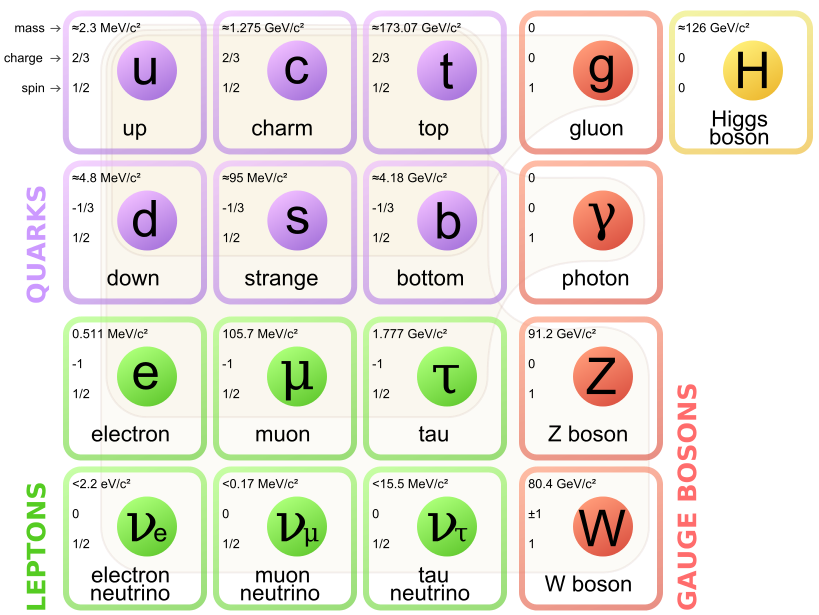
\includegraphics[width=0.6\textwidth]{figures/SM_particles}
  \caption{The particles of the Standard Model and their properties\cite{PDG}.}
  \label{fig:sm_particles}
\end{figure}

The Standard Model coalesced into a unified theoretical framework in the 1960s through the work of Glashow, Weinberg, Salam, and others on the theory of electroweak interactions\cite{Glashow, Weinberg, Salam, Glashow2}. This theory characterized both the electromagnetic and weak interactions as unified under a single gauge symmetry group, namely $SU(2) \times U(1)$. At low enough energy scales (on the order of the $W$ and $Z$ masses, the electroweak symmetry is broken, as evidenced by the fact that the weak bosons have mass while the photon does not. The discovery of the Higgs boson in 2012 confirmed the Higgs mechanism as the most likely candidate for this electroweak symmetry breaking\cite{Discovery, CMSDiscovery}. The electroweak theory is then combined with the theory of quantum chromodynamics (which models the strong sector as a non-abelian $SU(3)$ gauge group) to form the complete SM\cite{QCDBook}. 

\section{Electroweak Symmetry Breaking and the Higgs}

In the Standard Model Lagrangian, it is difficult to include mass terms for the $W$ and $Z$ bosons without breaking the fundamental gauge symmetry of the Lagrangian. A traditional mass term does not preserve the $SU(2) \times U(1)$ symmetry. Additionally, scattering of massive $W$ and $Z$ bosons violate unitarity and these diagrams diverge at high energy scales. In the 1960s, Higgs, Brout, Englert, Guralnik, Kibble, and Hagen developed a mechanism for spontaneous symmetry breaking via the additioanl of a complex scalar doublet to the SM. Three of the four real degrees of freedom of this complex field would go to the longitudinal modes of the $W^{\pm}$ and $Z$, thus allowing them to have mass\cite{Higgs1,Higgs2,Englert,Guralnik}. The remaining degree of freedom would manifest as an additional scalar, known now as the Higgs boson (Higgs was the first to predict the existence of the new particle). 

The mechanism works by introducing a Lagrangian for the newly introduced field that still respects the symmetry of the Standard Model inherently, but with a minimum at a non-zero vaccuum expectation value for the field. In this minimum of the potential, the electroweak symmetry is broken. Specifically, consider a complex scalar doublet $\phiH$ with four degrees of freedom, as shown in equation~\ref{eqn:phi_def}.

\begin{equation}
\label{eqn:phi_def}
\phiH = \left( \begin{array}{c} \phi^+ \\ \phi^0 \end{array} \right) = \frac{1}{\sqrt{2}}\left( \begin{array}{c} \phi_{1}^{+} + i\phi_{2}^+ \\ \phi_1^0 + i\phi_2^0 \end{array} \right)
%\phiH = \left( \begin{array}{c} \phi^+ \\ \phi^0  \end{array}\right) = \left( \begin{array}{c} \phi_1^+ + i\phi_2^+ \\ \phi_1^0 + i \phi_2^0 \end{array}\right) 
\end{equation}

The minimal potential of a self-interacting Higgs that still respects the SM symmetry is given in equation~\ref{eqn:potential}.

\begin{equation}
\label{eqn:potential}
V(\phiH) = \mu^2 \phiH^{\dagger}\phiH + \lambda(\phiH^\dagger\phiH)^2
\end{equation}

If the $\mu^2$ term of this potential is positive, then the potential has a minimum at $\phiH = 0$ and the SM symmetry is preserved. However, if instead $\mu^2 < 0$, then the minimum is at a finite value of $\phiH$, namely

\begin{equation}
\phiH_{\rm min} = \frac{1}{\sqrt{2}} \left(\begin{array}{c} 0 \\ v\end{array} \right)
\end{equation}

where $v = \sqrt{\mu^2/\lambda}$. Because this is the location of the minimum, it corresponds to the vacuum expectation value for the field ($\langle\phiH\rangle = \phiH_{\rm min}$). The excitations of the Higgs can then be parameterized as 

\begin{equation}
\phiH = \frac{1}{\sqrt{2}} \left(\begin{array}{c} 0 \\ v + H \end{array}\right)
\end{equation}

The full scalar Lagrangian, including the kinetic term, is then given as 

\begin{equation}
\mathcal{L}_s = (D^\mu \phiH)^\dagger(D_\mu\phiH) - V(\phiH)
\end{equation}

where the covariant derivative is defined as 

\begin{equation}
D_\mu = \partial_\mu + \frac{ig}{2}\tau^aW_\mu^a + ig'YB_\mu
\end{equation}

and $W^1, W^2, W^3$ and $B$ are the $SU(2)$ and $U(1)$ gauge fields of the electroweak theory, respectively. $g$ and $g'$ are the corresponding coupling constants. With the scalar Lagrangian in place, the physical gauge fields can then be written as 

\begin{equation}
\label{eqn:Weq}
W_\mu^\pm = \frac{1}{\sqrt{2}}(W_\mu^1 \mp iW_\mu^2) 
\end{equation}

\begin{equation}
\label{eqn:Zeq}
Z_\mu = \frac{-g'B_\mu + gW_\mu^3}{\sqrt{g^2 + g'^2}} 
\end{equation}

\begin{equation}
\label{eqn:photoneq}
A_\mu = \frac{gB_\mu + g'W_\mu^3}{\sqrt{g^2 + g'^2}}
\end{equation}

Equation~\ref{eqn:Weq} corresponds to the charged $W^+$ and $W^-$ bosons, equation~\ref{eqn:Zeq} corresponds to the neutral $Z$ boson, and equation~\ref{eqn:photoneq} corresponds to the neutral photon. The masses of the particles also arise from the Lagrangian. The photon has zero mass, while the masses of the $W$ and $Z$ bosons are given in equation~\ref{eqn:bosonmasses}.

\begin{equation}
\label{eqn:bosonmasses}
\begin{array}{c}
M_W^2 = \frac{1}{4}g^2v^2 \\ 
M_Z^2 = \frac{1}{4}(g^2 + g'^2)v^2
\end{array}
\end{equation}

The fermion masses also arise through a coupling with the Higgs via the Yukawa interaction (for a detailed description, see\cite{Dawson}). In this case the coupling between the Higgs and the fermions goes as 

\begin{equation}
\label{eqn:higgs-fermions}
g_{Hf\bar{f}} = \frac{m_f}{v}
\end{equation} 

The full Lagrangian of Higgs interactions can be written as 

\begin{equation}
\mathcal{L}_{\rm Higgs} = -g_{Hf\bar{f}}\bar{f}fH + \frac{g_{HHH}}{6}H^3 + \frac{g_{HHHH}}{24}H^4 + \delta_V V_\mu V^\mu\left(g_{HVV} H + \frac{g_{HHVV}}{2}H^2\right)
\end{equation}

with 

\begin{equation}
\begin{array}{cc}
g_{HVV} = \frac{2m_V^2}{v} & g_{HHVV} = \frac{2m_V^2}{v^2} \\ 
g_{HHH} = \frac{3m_H^2}{v} & g_{HHHH} = \frac{3m_H^2}{v^2}
\end{array}
\end{equation}

Here, $V$ refers to the $W^{\pm}$ and $Z$, and $\delta_{W} = 1$ while $\delta_Z = 1/2$. Phenomenologically, there are a few features of this Lagrangian that are useful to note. First, note that the Higgs mass is a free parameter of the theory that must be determined experimentally. Second, note that the coupling of the Higgs to the vector bosons and fermions scales with the masses of these particles, a fact that is important when considering both the production and decays of the particle. Also note that the branching ratio of the Higgs to $W$ bosons will be twice that of the branching ratio to $Z$ if the Higgs mass is large enough to produce the particles on shell because of the extra symmetry factor associated with the $W$ coupling. Finally, note the presence of the cubic and quartic Higgs self interaction terms, which can lead to final states with multiple Higgs bosons produced. 

\section{Higgs Boson Production and Decay}

This section discusses the properties of Higgs production and decay mechanisms. The details presented here will focus on the properties of a $125 \GeV$ Higgs boson, as this is the mass closest to that of the newly discovered Higgs. 

\subsection{Higgs production}

The Higgs is produced by four main production modes at the Large Hadron Collider - gluon-gluon fusion (ggF), vector boson fusion (VBF), associated production with a $W$ or $Z$ boson, or associated production with top quarks ($\ttbar H$). Figure~\ref{fig:production_modes} shows the Feynman diagrams for these four modes. 

\begin{figure}[h!]
  %\vspace{20pt}
  \centering
  \captionsetup{justification=centering}

   \begin{subfigure}[t]{0.5\textwidth}
        \centering
        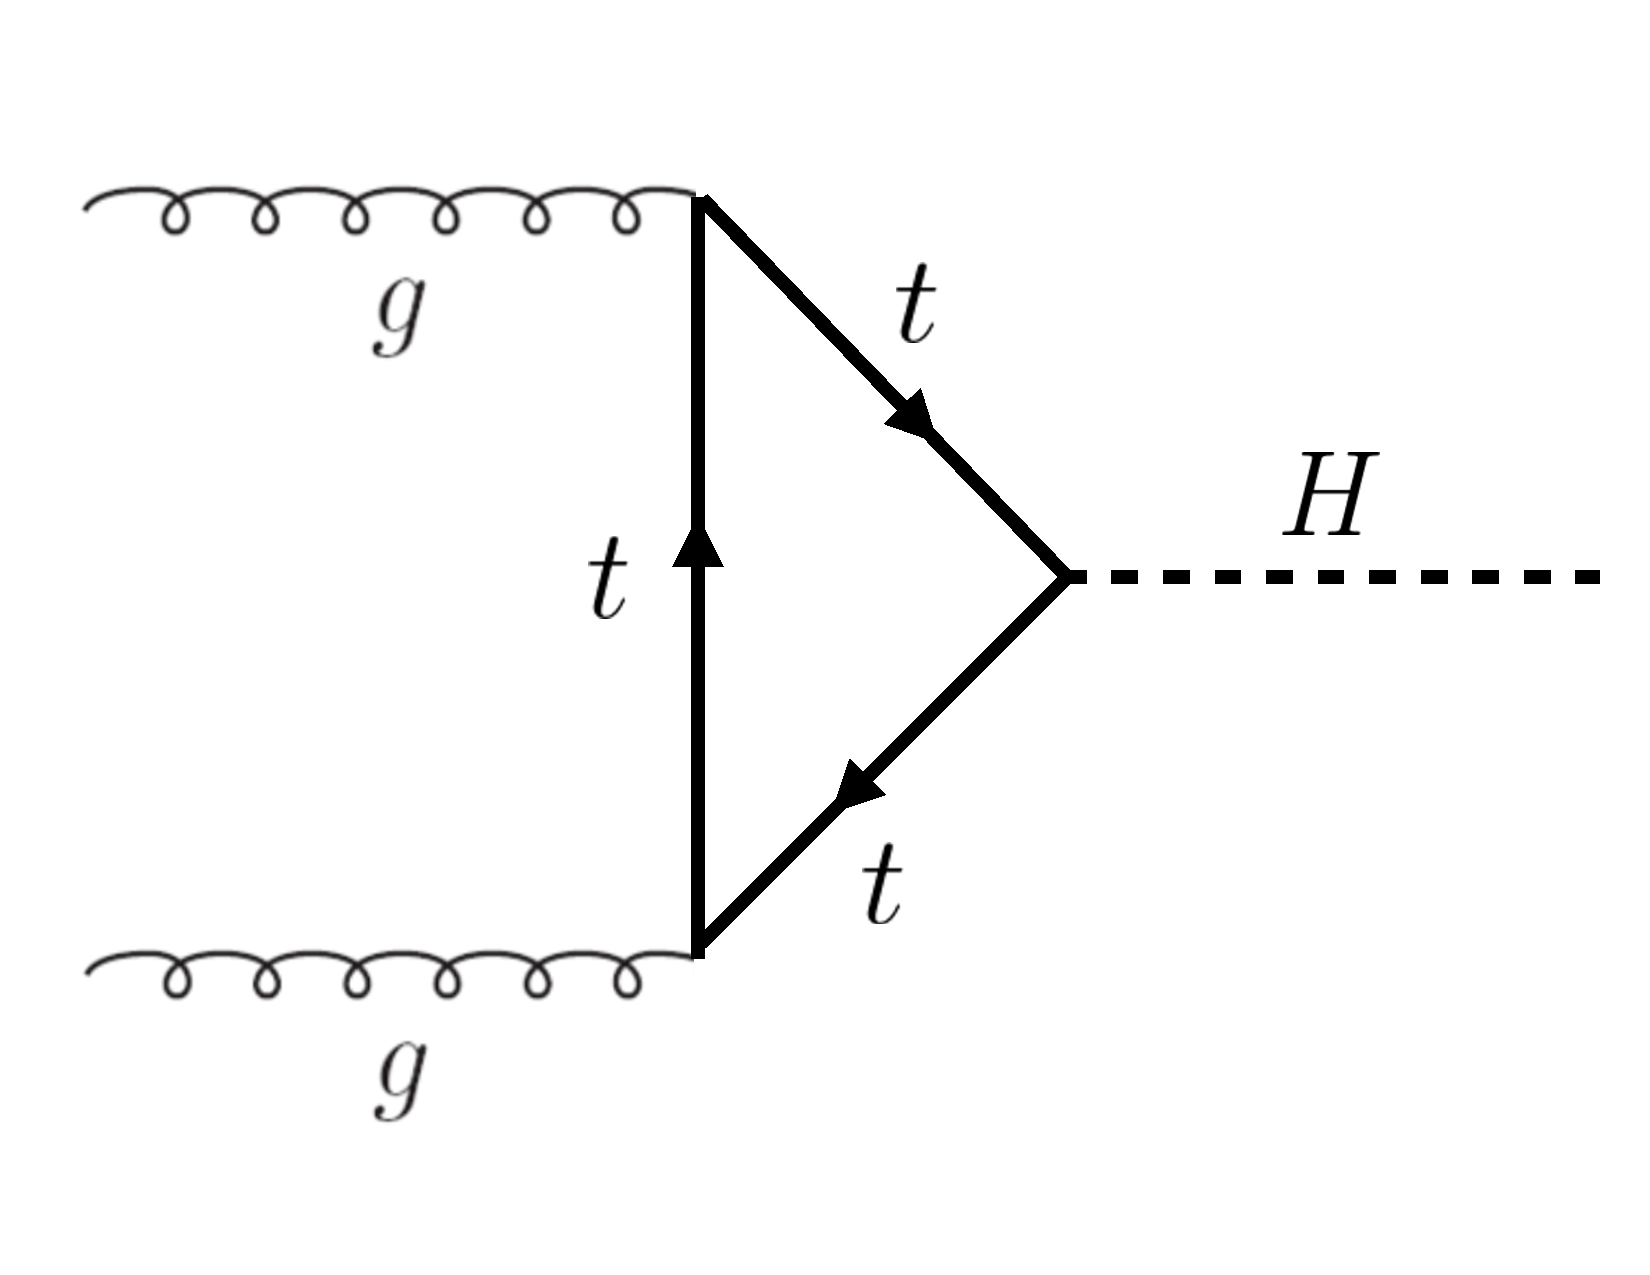
\includegraphics[width=0.6\textwidth]{figures/ggF_Higgs}
        \caption{}
    \end{subfigure}%
    \begin{subfigure}[t]{0.5\textwidth}
        \centering
        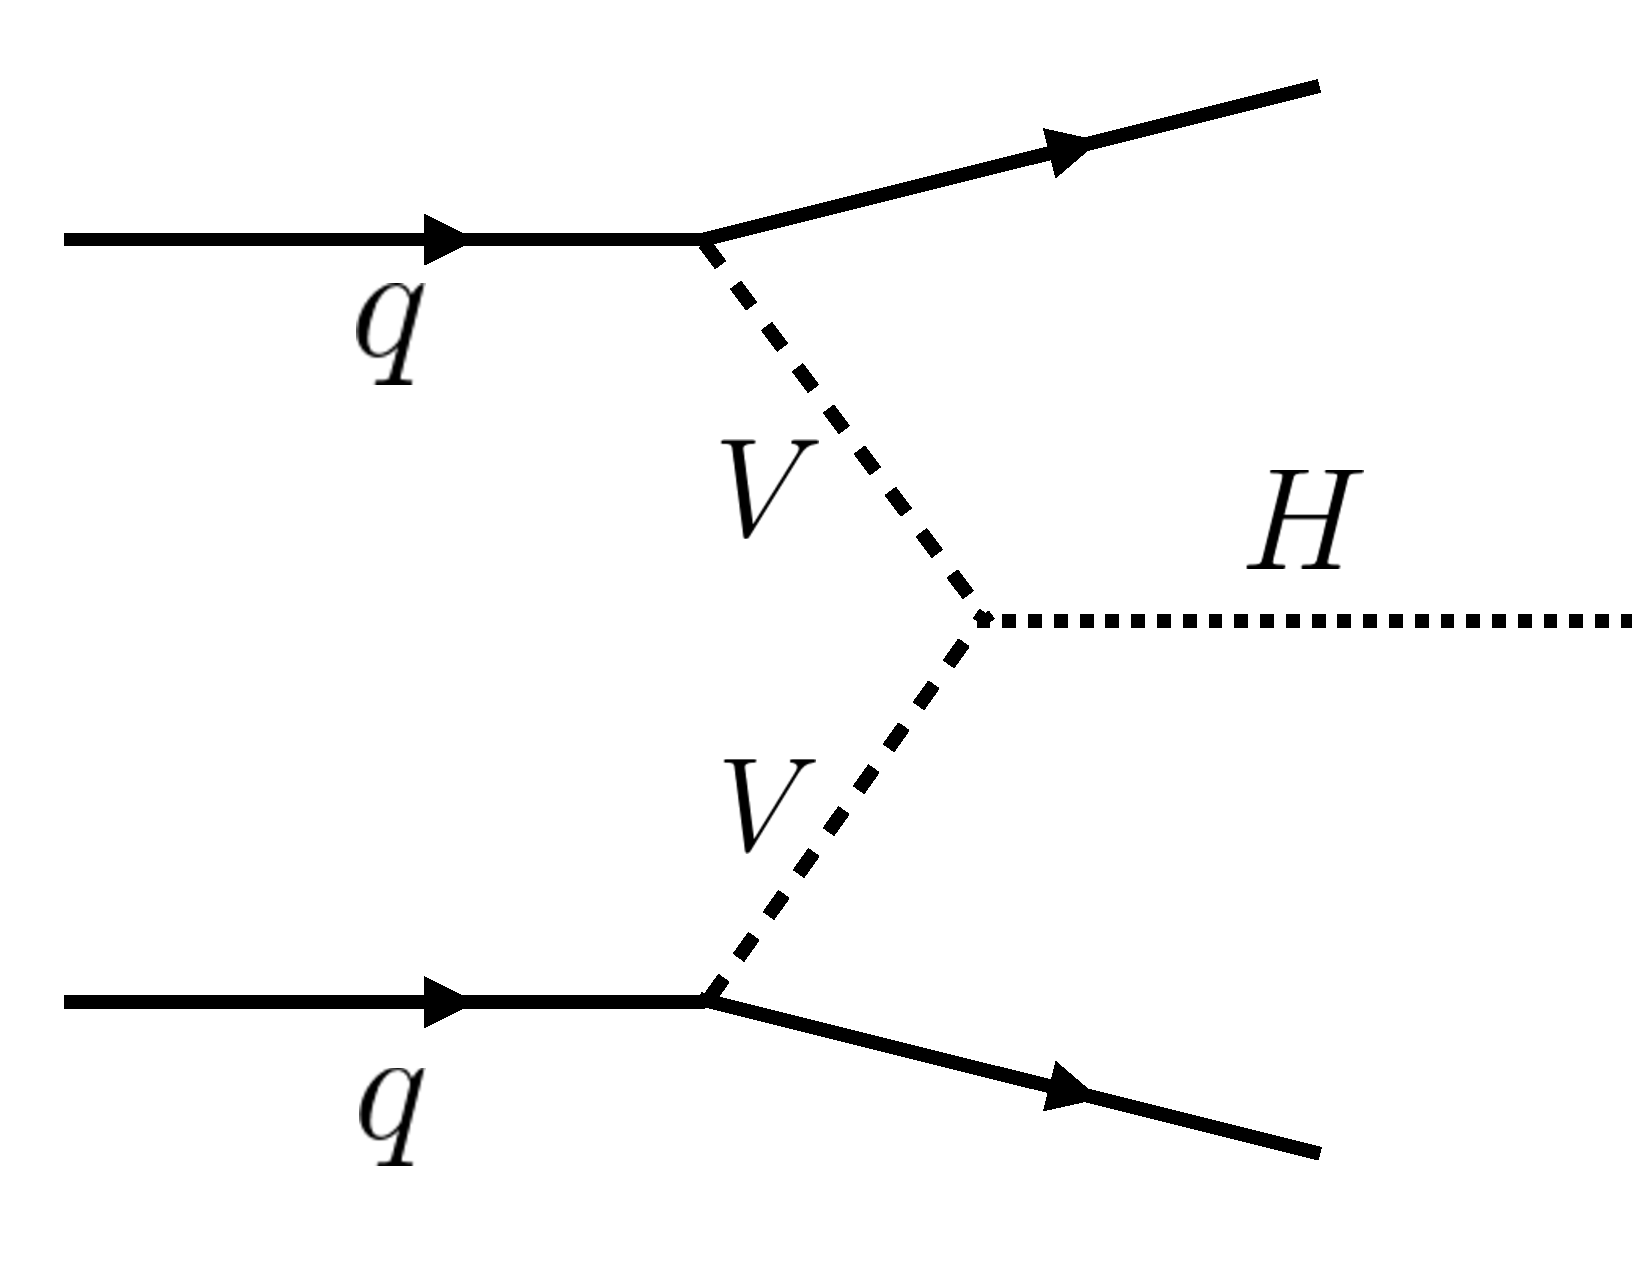
\includegraphics[width=0.6\textwidth]{figures/VBF_Higgs}
        \caption{}
    \end{subfigure}

    \begin{subfigure}[t]{0.5\textwidth}
        \centering
        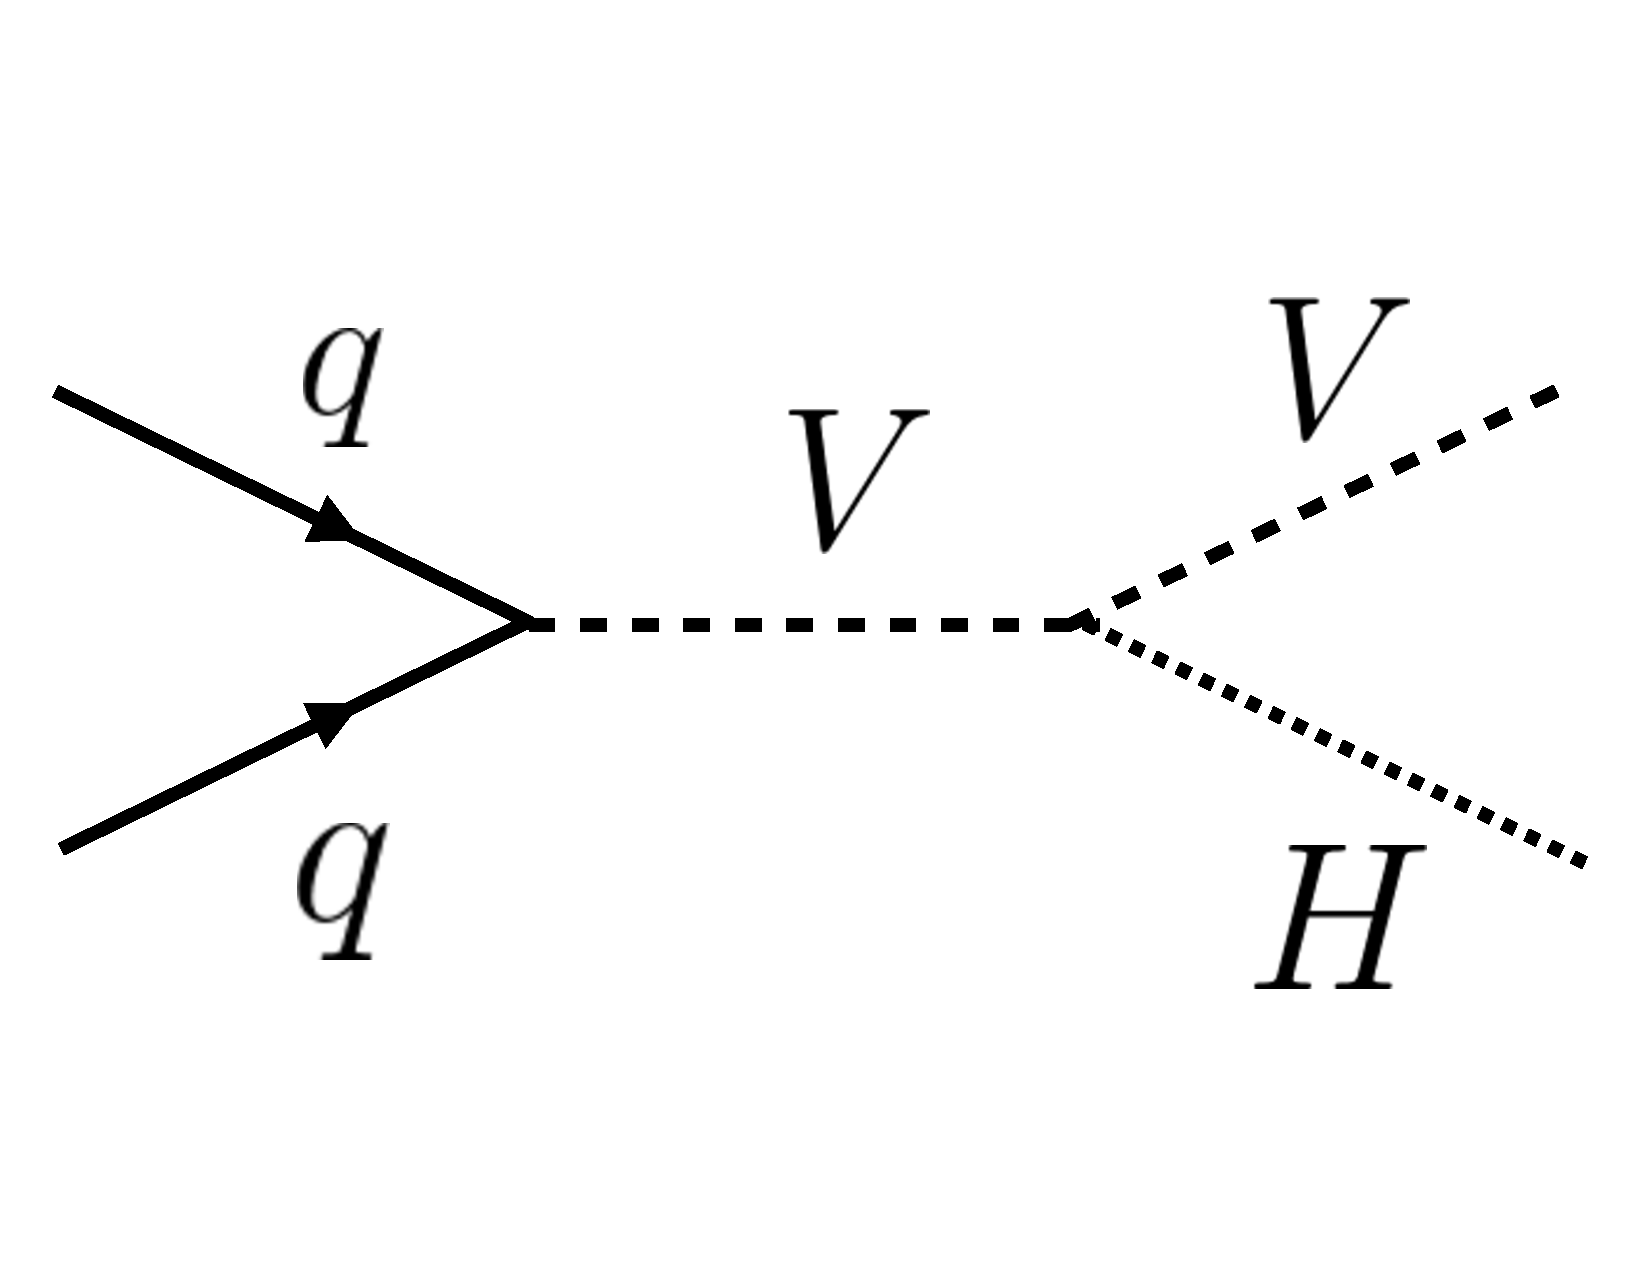
\includegraphics[width=0.6\textwidth]{figures/V_higgs}
        \caption{}
    \end{subfigure}%
    \begin{subfigure}[t]{0.5\textwidth}
        \centering
        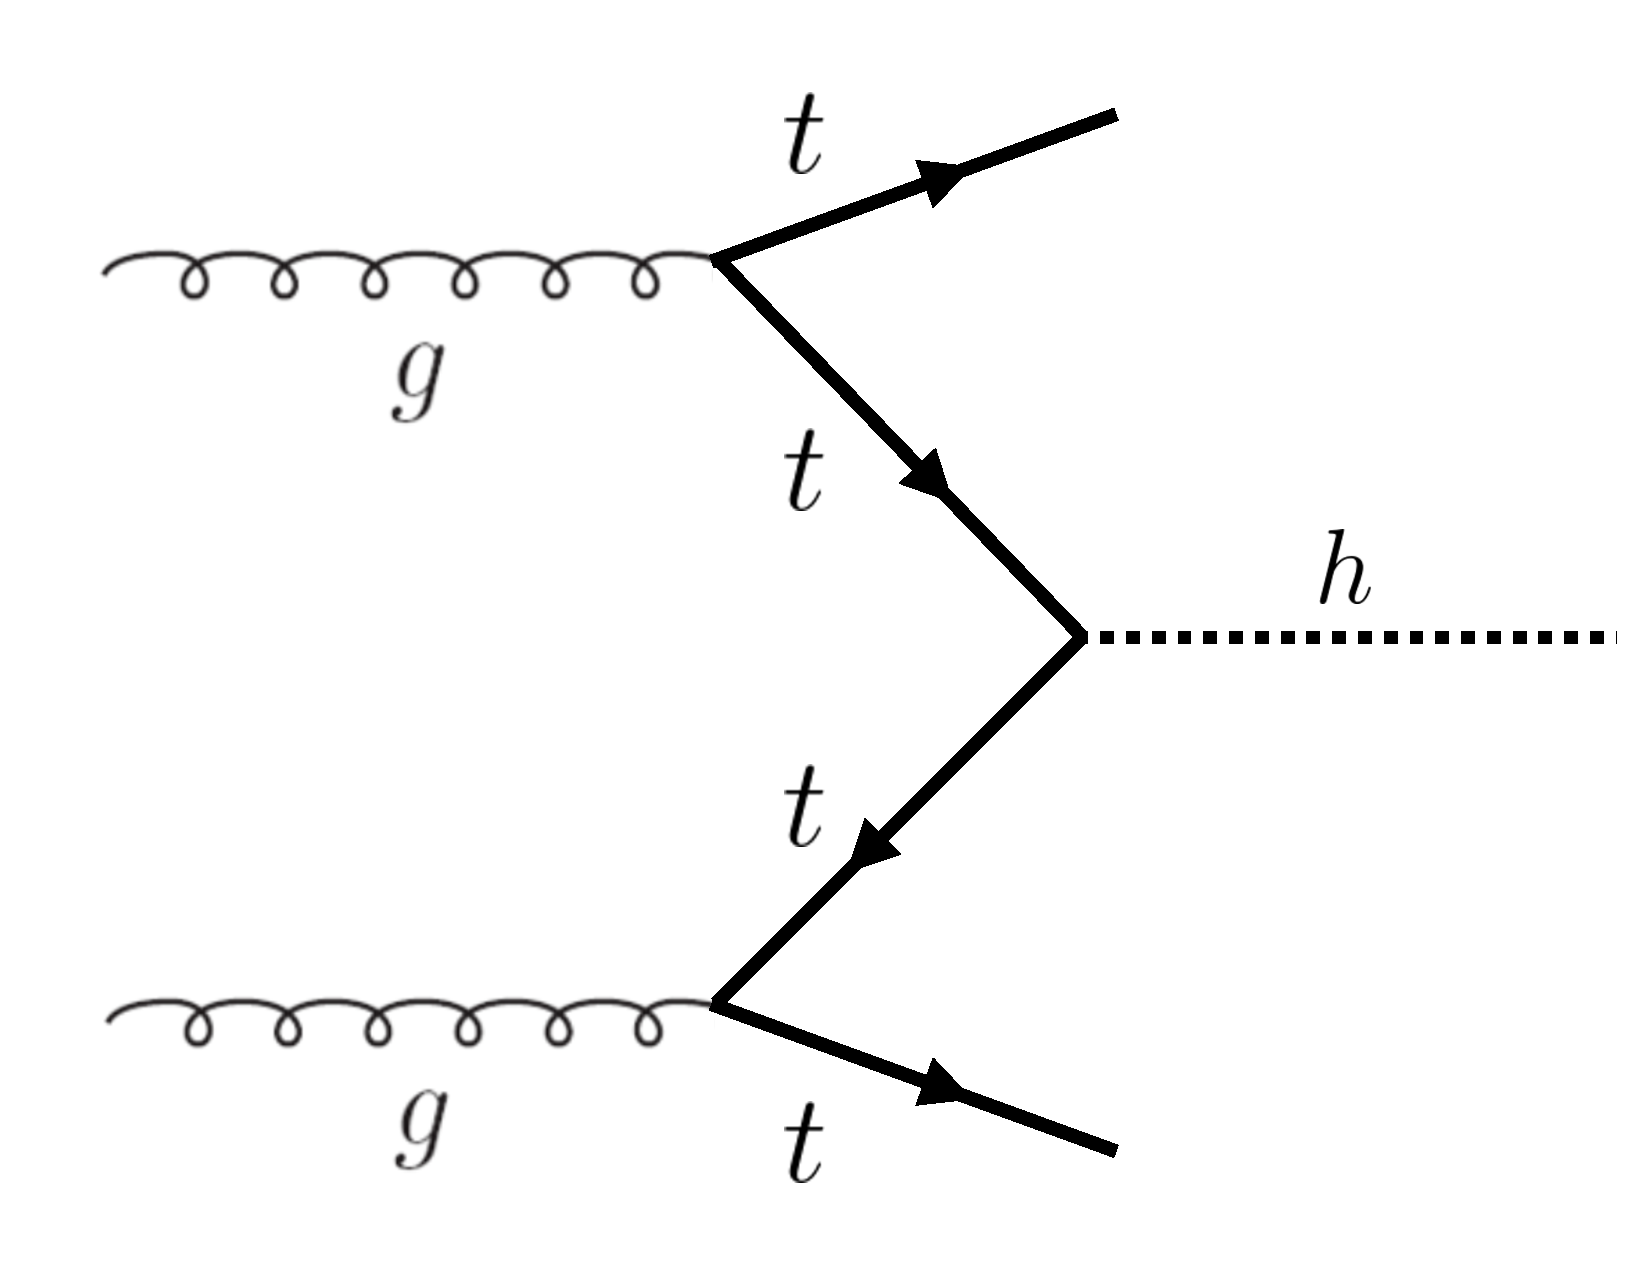
\includegraphics[width=0.6\textwidth]{figures/ttH}
        \caption{}
    \end{subfigure}

   \caption{The four most common Higgs boson production modes at the LHC: (a) gluon-gluon fusion, (b) vector boson fusion, (c) $W/Z$ + $H$ production, (d) $\ttbar H$ production}
  \label{fig:production_modes}
\end{figure}

In gluon-gluon fusion, gluons from the incoming protons fuse via a top-quark loop to produce a Higgs. The top quark is the dominant contribution in the loop due to its heavy mass and the fact that the Higgs-fermion coupling constant scales with fermion mass. In vector boson fusion, the incoming quarks each radiate a $W$ or $Z$ boson which fuse to produce the Higgs. This production mode results in a final state with a Higgs boson and two addtional jets which tend to be forward because they carry the longtiduinal momentum of the incoming partons. The Higgs can also be produced in associated with a $W$ or $Z$ boson. The $W/Z$ is produced normally and then radiates a Higgs (this mode is also sometimes known as ``Higgs-strahlung"). Finally, the Higgs can be produced in association with two top quarks. Each incoming gluon splits into a $\ttbar$ pair, and one of the top pairs combines to create a Higgs. 

Figure~\ref{fig:Higgs_xsec} shows the production cross section for a $125 \GeV$ Higgs boson in each of these modes at a $pp$ collider as a function of center of mass energy. 

\begin{figure}[h!]
  %\vspace{20pt}
  \centering
  \captionsetup{justification=centering}

  %\hspace*{-32pt}
  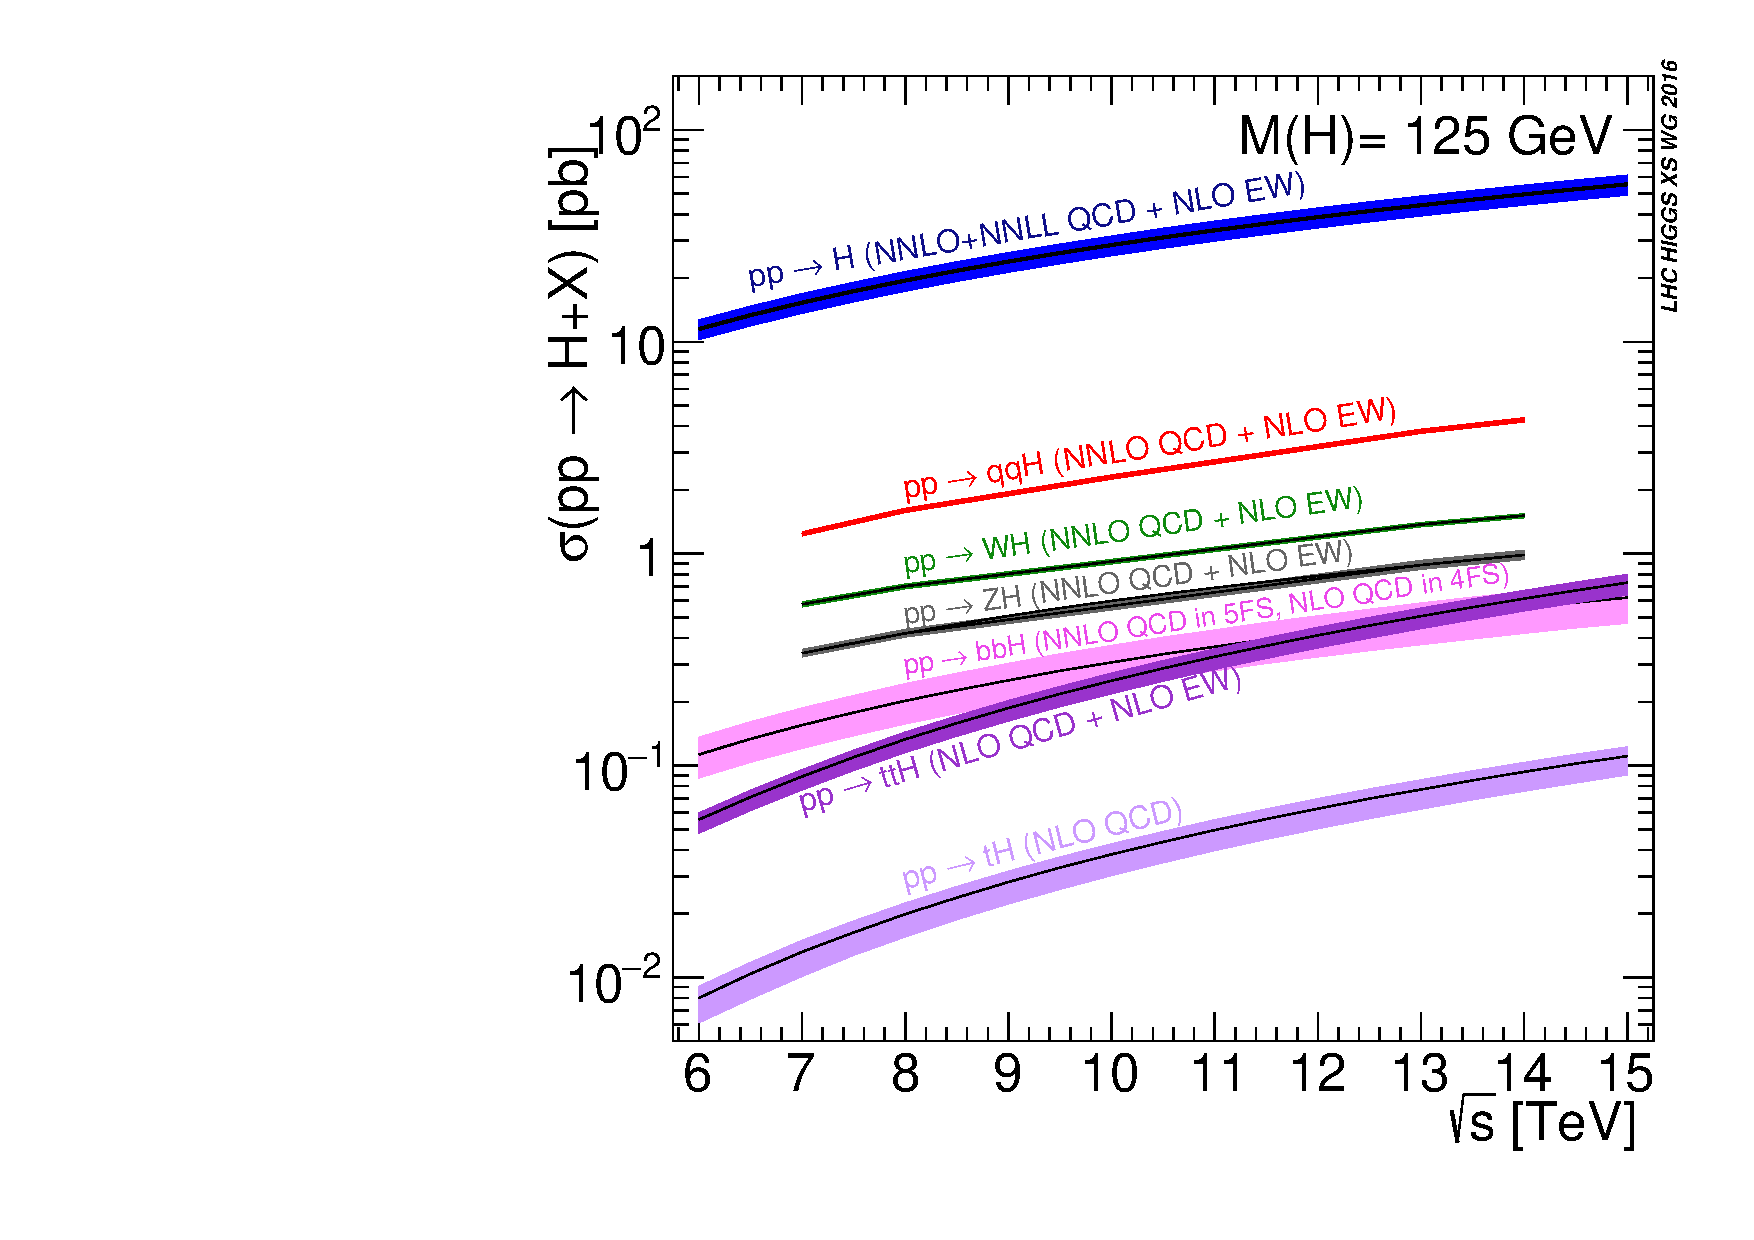
\includegraphics[width=0.6\textwidth,angle=270]{figures/h125_xsec}
  \caption{Higgs production cross sections as a function of center of mass energy ($\sqrt{s}$) at a $pp$ collider\cite{LHCXSWG}.}
  \label{fig:Higgs_xsec}
\end{figure}

In figure~\ref{fig:Higgs_xsec}, note that gluon fusion has the largest cross section, while VBF is the second largest at approximately a factor of $10$ smaller. The figure also includes the less commonly studied $b\bar{b}H$ and $tH$ modes. The $b\bar{b}H$ and $tH$ modes are not studied as commonly as $t\bar{t}H$ due to the larger background contributions and lower cross sections, respectively. At $\sqrt{s} = 8 \TeV$, ggF production of a $125 \GeV$ Higgs has a cross section of $19.47 \pb$, while VBF has a cross section of $1.601 \pb$\cite{LHCXSWG}. The cross sections of all of the main Higgs production modes at this center of mass energy, as well as their uncertainties from varying the renormalization and factorization scales and PDFs, are summarized in table~\ref{tab:Higgs_xsec} for a $125 \GeV$ Higgs.

\begin{table}[h!]
\centering
\captionsetup{justification=centering}
%\begin{tabular*}{0.480\textwidth}{p{0.075\textwidth} p{0.180\textwidth} l}
\hspace{-10pt}
\begin{tabular}{|c|c|c|c|}
\hline
Production mode & $\sigma$ (\pb) & \specialcell{QCD scale \\ uncert. (\%)} & \specialcell{PDF + $\alpha_s$  \\ uncert. (\%)} \\ \hline
Gluon fusion & $19.47$ & $+7.3/-8.0$ & $3.1$ \\ \hline
Vector boson fusion & $1.601$ & $+0.3/-0.2$ & $2.2$ \\ \hline
$WH$ & $0.7026$ & $+0.6/-0.9$ & $2.0$ \\ \hline
$ZH$ & $0.4208$ & $+2.9/-2.4$ & $1.7$ \\ \hline
$t\bar{t} H$ & $0.1330$ & $+4.1/-9.2$ & $4.3$ \\ \hline
$b\bar{b} H$ & $0.2021$ & \multicolumn{2}{c|}{$+20.7/-22.3$} \\ \hline
$tH$ ($t$-channel) & $0.01869$ & $+7.3/-16.5$ & $4.6$ \\ \hline
$tH$ ($s$-channel) & $1.214\times 10^{-3}$ & $+2.8/-2.4$ & $2.8$ \\ \hline
\end{tabular}

\caption{
Production cross sections for a $125 \GeV$ Higgs boson at $\sqrt{s} = 8 \TeV$ with scale and PDF uncertainties~\cite{LHCXSWG}. 
}
\label{tab:Higgs_xsec}
\end{table}



\subsection{Higgs branching ratios}

The fact that the Higgs couples more strongly to more massive particles is crucial for understanding its branching ratios. The width for Higgs decays to fermions is given in equation~\ref{eqn:Hff_width}~\cite{Tully}.

\begin{equation}
\label{eqn:Hff_width}
\Gamma(H\to f\bar{f}) = \frac{N_c \sqrt{2} G_F m_f^2 m_H}{8\pi}
\end{equation}

In this case, $N_c$ is the number of colors, $G_F$ is the Fermi constant, $m_f$ is the mass of the fermion, and $m_H$ is the mass of the Higgs. Note that the width scales with the square of the fermion mass. (This also assumes that the Higgs mass is large enough to decay with both the fermions on shell.) 

The decay width to $WW$ is given in equation~\ref{eqn:HWW_width}~\cite{Tully}. 

\begin{equation}
\label{eqn:HWW_width}
\Gamma(H\to W^+W^-) = \frac{\sqrt{2} G_F M_W^2 m_H}{16\pi}\frac{\sqrt{1-x_W}}{x_W}\left(3x_W^2 - 4x_W + 4\right)
\end{equation}

where $m_W$ is the mass of the $W$ and $x_W  = 4M_W^2/m_H^2$. To get the branching ratio to $ZZ$, the equation is divided by $2$ to account for identical particles in the final state, and $x_W$ is replaced with $x_Z = 4M_Z^2/m_H^2$. This is shown in equation~\ref{eqn:HZZ_width}~\cite{Tully}.

\begin{equation}
\label{eqn:HZZ_width}
\Gamma(H\to ZZ) = \frac{\sqrt{2} G_F M_Z^2 m_H}{32\pi}\frac{\sqrt{1-x_Z}}{x_Z}\left(3x_Z^2 - 4x_Z + 4\right)
\end{equation}

These formulas can also be visualized as a function of Higgs mass. Figure~\ref{fig:branching_ratios} shows the branching ratios as a function of the Higgs mass. 

\begin{figure}[h!]
  %\vspace{20pt}
  \centering
  \captionsetup{justification=centering}
  %\hspace*{-32pt}
  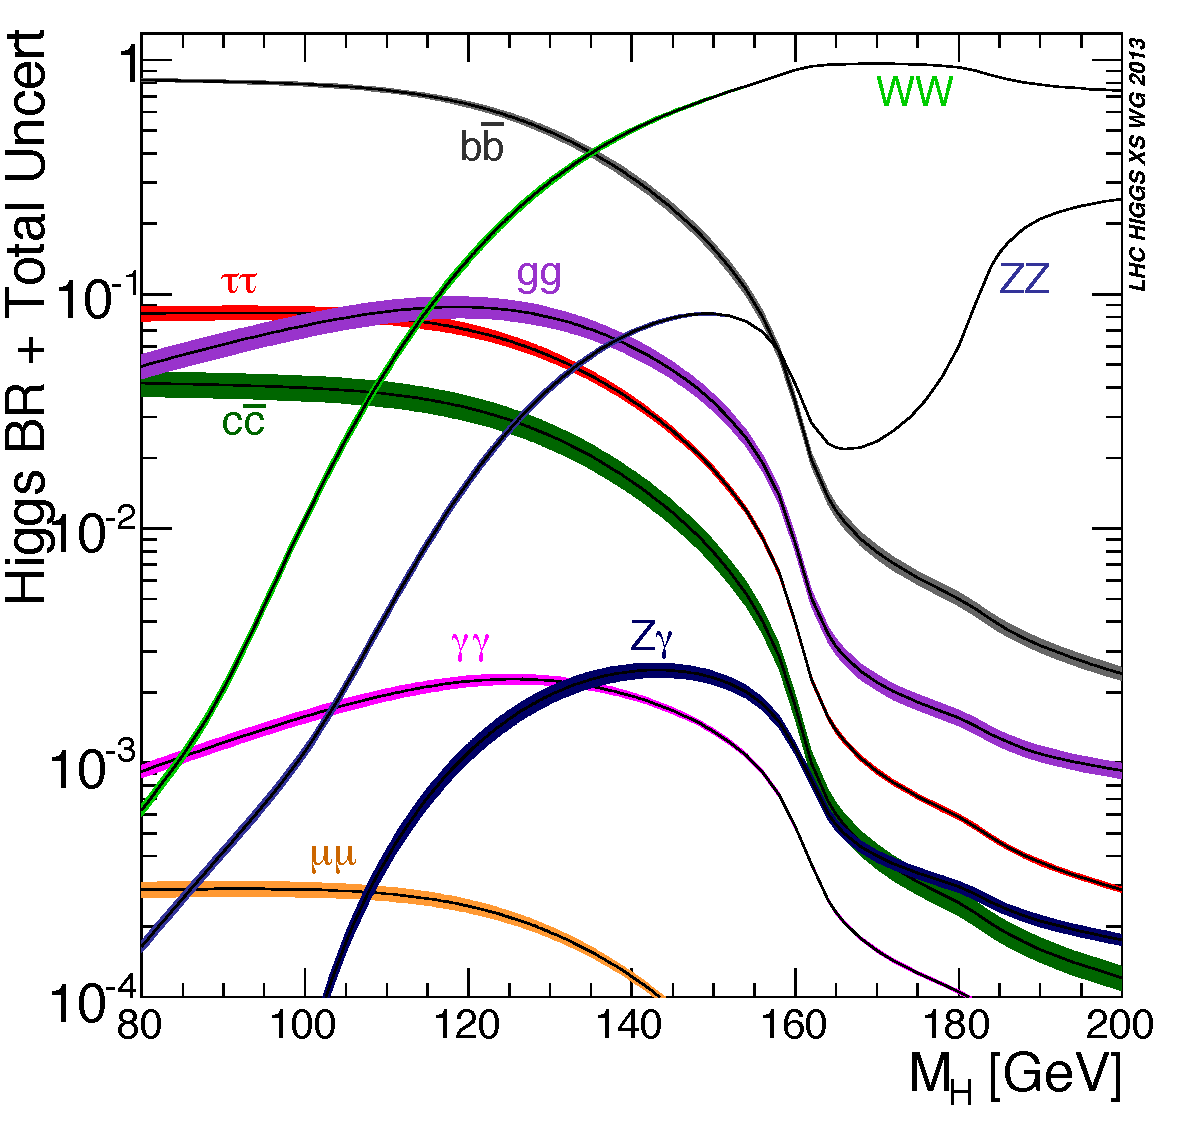
\includegraphics[width=0.6\textwidth]{figures/Higgs_BR}
  \caption{Higgs boson branching ratios as a function of $m_H$\cite{LHCXSWG}.}
  \label{fig:branching_ratios}
\end{figure}

There are a few interesting features to note in this figure. First, note that at high Higgs masses, once on-shell production of both $W$ and $Z$ bosons is possible, these two decays are the dominant ones due to the large masses of the $W/Z$. Also note that the branching ratio to $W$s is twice that of $Z$s at these large masses due to the $\delta_V$ symmetry factor noted previously. At $125 \GeV$, the Higgs is accessible through many different decay modes. The largest branching ratio is the decay $H\to b\bar{b}$ at 58.24\%~\cite{LHCXSWG}. This branching is larger than the $WW$/$ZZ$ decays because one of the two bosons must be produced off-shell for $m_H = 125 \GeV$. The second largest branching ratio is to $WW^*$ at $21.37$ \% (before taking into account the branching ratios of the $W$). Table~\ref{tab:Higgs_BR} summarizes the branching ratios for a $125 \GeV$ Higgs. Note that there is in fact a Higgs branching ratio to $\gamma\gamma$ even though photons are massless. This decay happens through a loop (the largesst contributions to the loop are top and $W$) which suppresses the branching ratio. 

\begin{table}[h!]
\centering
\captionsetup{justification=centering}

%\begin{tabular*}{0.480\textwidth}{p{0.075\textwidth} p{0.180\textwidth} l}
\hspace{-10pt}
\begin{tabular}{|c|c|}
\hline
Decay & Branching ratio (\%) \\ \hline
$b\bar{b}$ & $58.24$ \\ \hline
$WW^*$ & $21.37$ \\ \hline
$gg$ & $8.187$ \\ \hline
$\tau\tau$ & $6.272$ \\ \hline
$c\bar{c}$ & $2.891$ \\ \hline
$ZZ^*$ & $2.619$ \\ \hline
$\gamma\gamma$ & $0.2270$ \\ \hline
$Z\gamma$ & $0.1533$ \\ \hline
$\mu\mu$ & $0.02176$ \\ \hline
\end{tabular}

\caption{
Branching ratios for a $125 \GeV$ Higgs boson\cite{LHCXSWG}. 
}
\label{tab:Higgs_BR}
\end{table}


Note that the branching ratios alone do not tell the full story of which Higgs channels are the most sensitive. For example, a $H\to b\bar{b}$ search in gluon fusion production is incredibly difficult due to the large QCD dijet background at the LHC. However, in associated production of the Higgs, where a $W$ or $Z$ gives additional final state particles that can be used to reduce background, a search for $H\to b\bar{b}$ can be sensitive. The combinations of production and decay modes that are most commonly studied are summarized in table~\ref{tab:sensitive_channels}~\cite{Tully}.

\begin{table}[h!]
\centering
\captionsetup{justification=centering}

%\begin{tabular*}{0.480\textwidth}{p{0.075\textwidth} p{0.180\textwidth} l}
\begin{tabular}{|c|c|c|c|c|}
\hline
Decay & Inclusive (incl. ggF) & VBF & $WH/ZH$ & $t\bar{t}H$ \\ \hline
$H\to\gamma\gamma$ & \checkmark & \checkmark & \checkmark & \checkmark \\ \hline
$H\to b \bar{b}$ & & & \checkmark & \checkmark \\ \hline
$H\to \tau^+\tau^-$ & & \checkmark & & \\ \hline
\HWWfull & \checkmark & \checkmark & \checkmark &  \\ \hline
$H \to ZZ \to 4\ell$ & \checkmark & & & \\ \hline
$H \to Z\gamma \to \ell\ell\gamma$ & very low & & & \\ \hline
\end{tabular}

\caption{
Possible channels for Higgs searches. Checkmarks denote the most sensitive production modes~\cite{Tully}. 
}
\label{tab:sensitive_channels}
\end{table}

\section{Higgs Pair Production in the Standard Model}

The Standard Model also allows for processes that produce two Higgs bosons in the final state, known as Higgs pair production or di-Higgs production. The two main production mechanisms are shown in figure~\ref{fig:diHiggs}.

\begin{figure}[h!]
  %\vspace{20pt}
  \centering
  \captionsetup{justification=centering}

   \begin{subfigure}[t]{0.5\textwidth}
        \centering
        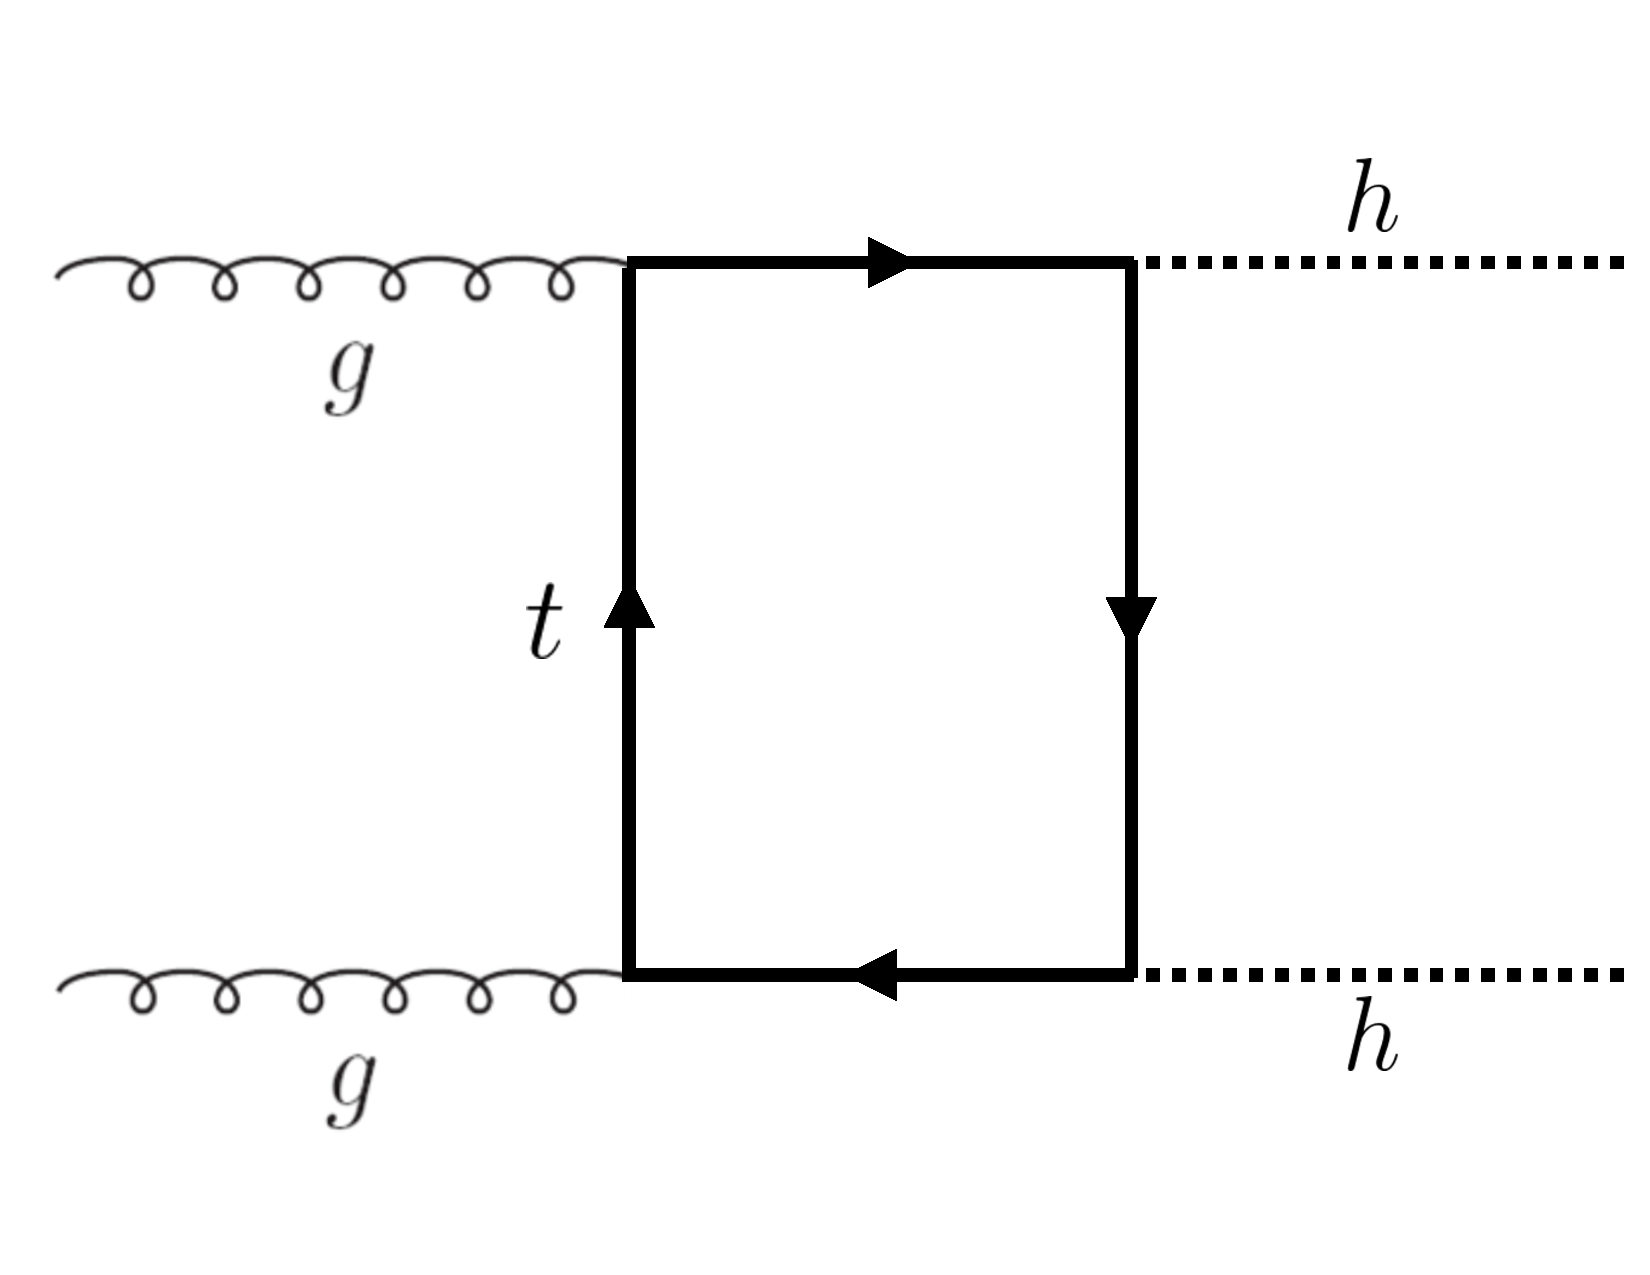
\includegraphics[width=0.7\textwidth]{figures/HH_box}
        \caption{}
    \end{subfigure}%
    \begin{subfigure}[t]{0.5\textwidth}
        \centering
        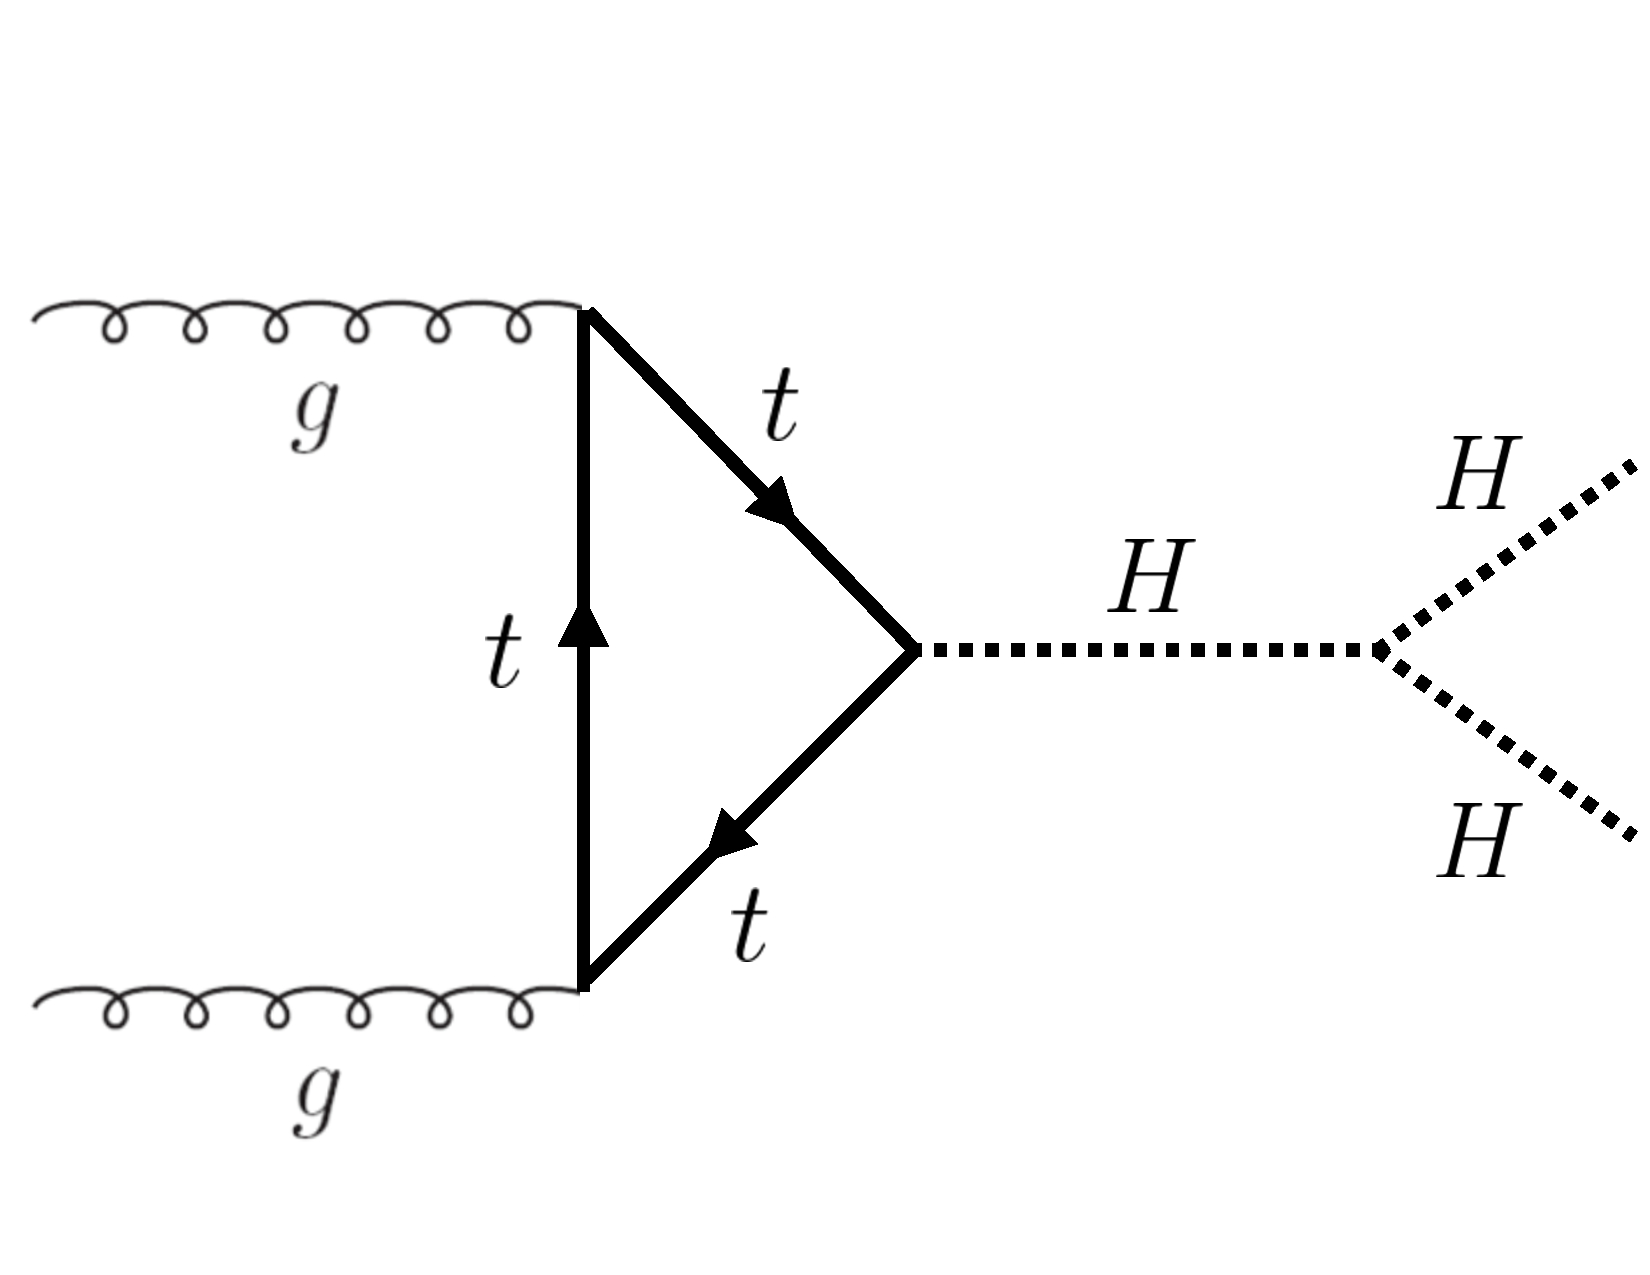
\includegraphics[width=0.7\textwidth]{figures/HH_lambda}
        \caption{}
    \end{subfigure}
   \caption{The two leading diagrams for Standard Model di-Higgs production at the LHC: (a) box diagram, (b) Higgs self coupling}
  \label{fig:diHiggs}
\end{figure}

The two diagrams in figure~\ref{fig:diHiggs} interfere destructively with one another, resulting in a low overall cross section for di-Higgs production at the LHC. Nevertheless, Higgs pair production is quite interesting to study because it gives direct access to the $\lambda$ parameter of the Higgs potential, also known as the Higgs self coupling. The diagram in figure~\ref{fig:diHiggs}(b) is sensitive to this coupling through the triple Higgs vertex.  

One can substitute the gluon fusion production of diagram~\ref{fig:diHiggs}(b) with any of the other production modes previously discussed. These other modes do not suffer from interference with the box diagram in figure~\ref{fig:diHiggs}(a) due to the presence of additional particles in the final state. They still have a lower cross section than the gluon fusion mode, however. The cross sections for di-Higgs production in the different modes, as well as their uncertainties, are shown in table~\ref{tab:diHiggs_xsec}~\cite{HH_LHC}. These are shown for $\sqrt{s} = 14 \TeV$ as the higher center of mass energy is more sensitive to this process. Note that the scale of cross section quoted is now in $\fb$ rather than $\pb$.
\begin{table}[h!]
\centering
\captionsetup{justification=centering}
%\begin{tabular*}{0.480\textwidth}{p{0.075\textwidth} p{0.180\textwidth} l}
\hspace{-10pt}
\begin{tabular}{|c|c|c|}
\hline
Production mode & $\sigma$ (\fb) & \specialcell{Total \\ uncert. (\%)} \\ \hline
Gluon fusion & $33.89$ & $+37.2/-27.8$  \\ \hline
Vector boson fusion & $2.01$ & $+7.6/-5.1$  \\ \hline
$WHH$ & $0.57$ & $+3.7/-3.3$ \\ \hline
$ZHH$ & $0.42$ & $+7.0/-5.5$ \\ \hline
$t\bar{t} H$ & $1.02$ & - \\ \hline
\end{tabular}

\caption{
Production cross sections for pair production of a $125 \GeV$ Higgs boson at $\sqrt{s} = 14 \TeV$ with total uncertainty~\cite{HH_LHC}. The uncertainties include QCD scale and PDF variations as well as uncertainties on $\alpha_S$. 
}
\label{tab:diHiggs_xsec}
\end{table}

\section{Higgs Pair Production in Theories Beyond the Standard Model}

The Standard Model Higgs pair production cross section is rather small, and datasets on the scale of the full lifetime of the LHC will be required to obtain sensitive measurements of the Higgs self-coupling. However, the discovery of the Higgs also gives particle physicists a new tool that can be exploited in the search for new physics beyond the Standard Model. In particular, Higgs pair production is a promising channel in the search for new physics. The cross section for di-Higgs production can be altered through both resonant and non-resonant production of Higgs pairs. In non-resonant production, di-Higgs production vertices can arise from the presence of a new strong sector and additional colored particles\cite{HH_NewPhys,AnomalousHHVertex,CompositeDiHiggs}. Figure~\ref{fig:HH_nonres} shows examples of the types of vertices that can arise. In the resonant case, new heavy particle can decay to Higgs pairs. Such new particles can include heavy Higgs bosons arising in two Higgs doublet models (2HDM) or Higgs portal models as well as heavy gravitons in Randall-Sundrum theories\cite{HH_NewPhys,RSG1,RSG_LHC,RSG_LHC2,HH_2HDM,2HDM2,HiggsPortal}. Figure~\ref{fig:HH_res} shows a generic diagram for a heavy resonance decaying to two Higgs bosons. In the 2HDM, $X$ corresponds to the heavy CP-even scalar $H$. In the Randall-Sundrum model, $X$ corresponds to a heavy spin-2 graviton $G$. 


\begin{figure}[h!]
  %\vspace{20pt}
  \centering
  \captionsetup{justification=centering}

  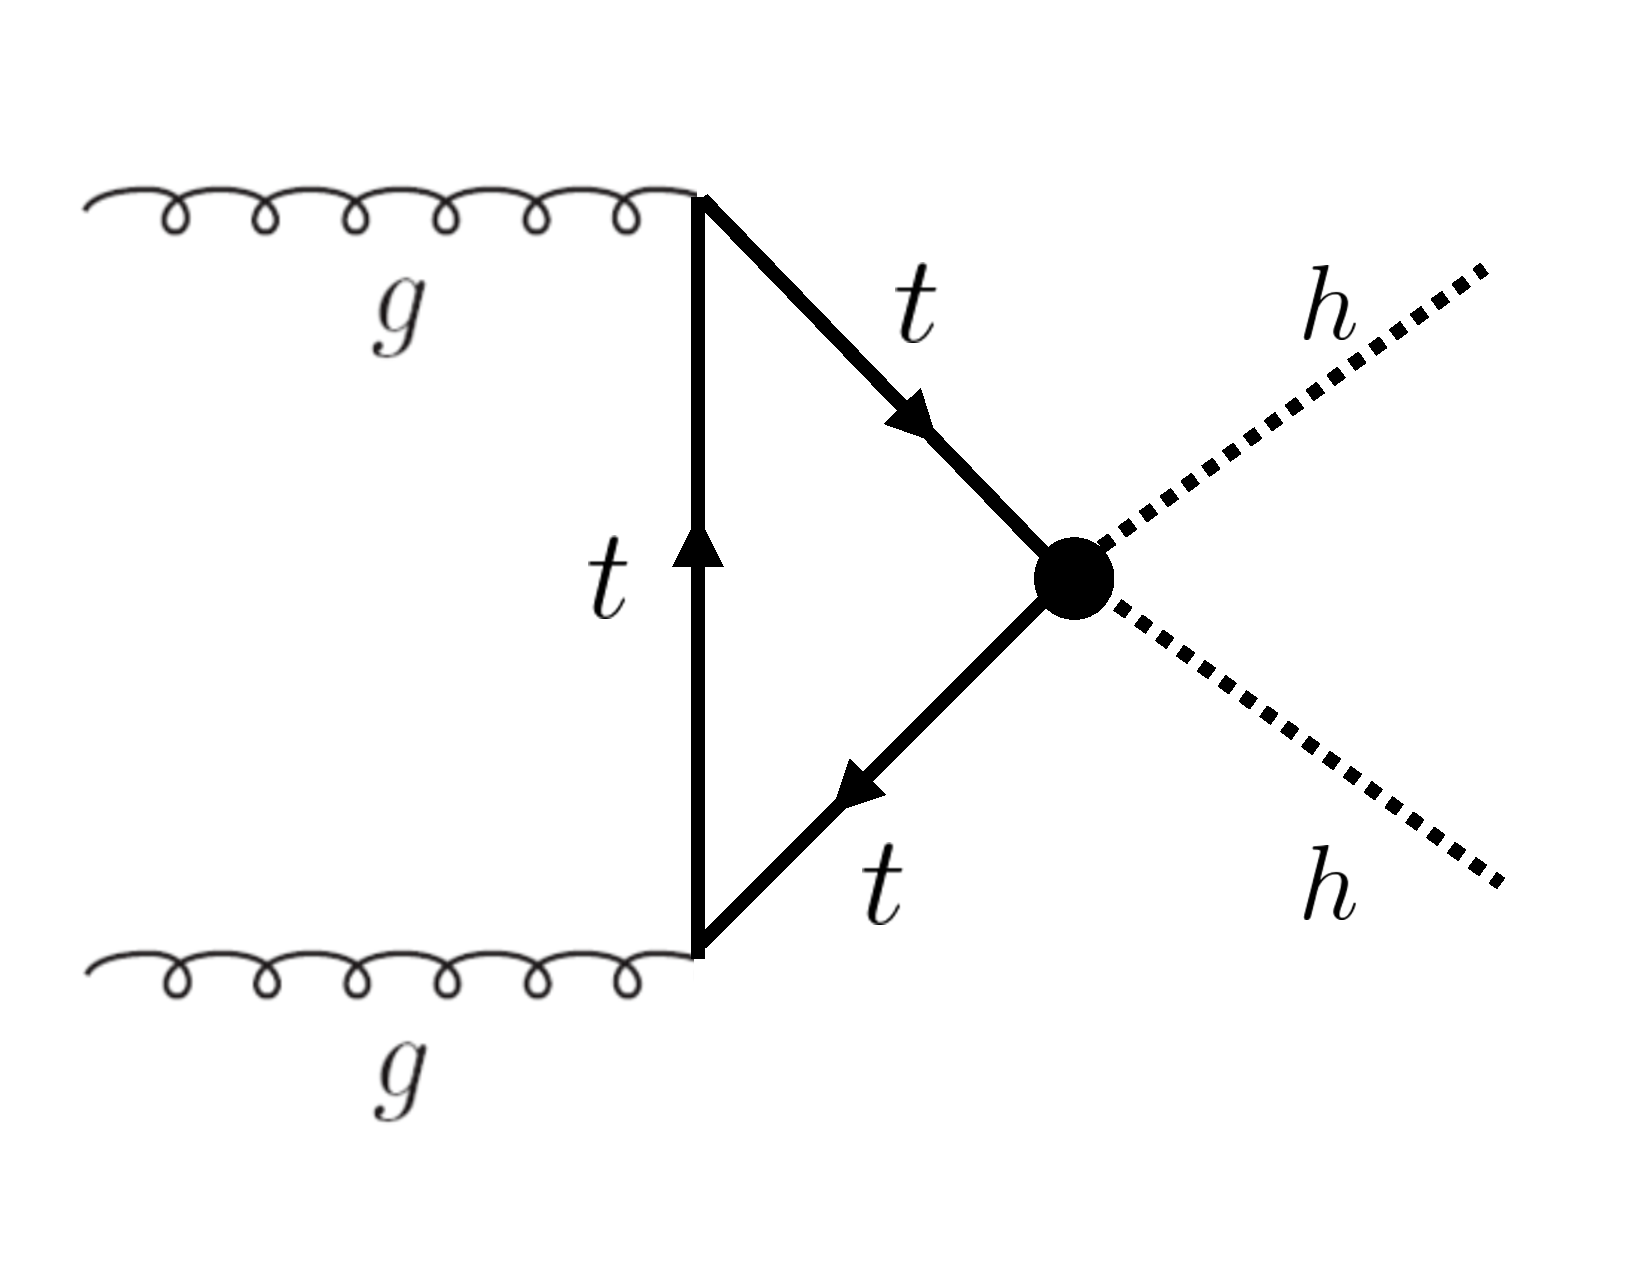
\includegraphics[width=0.4\textwidth]{figures/HH_nonres1}
  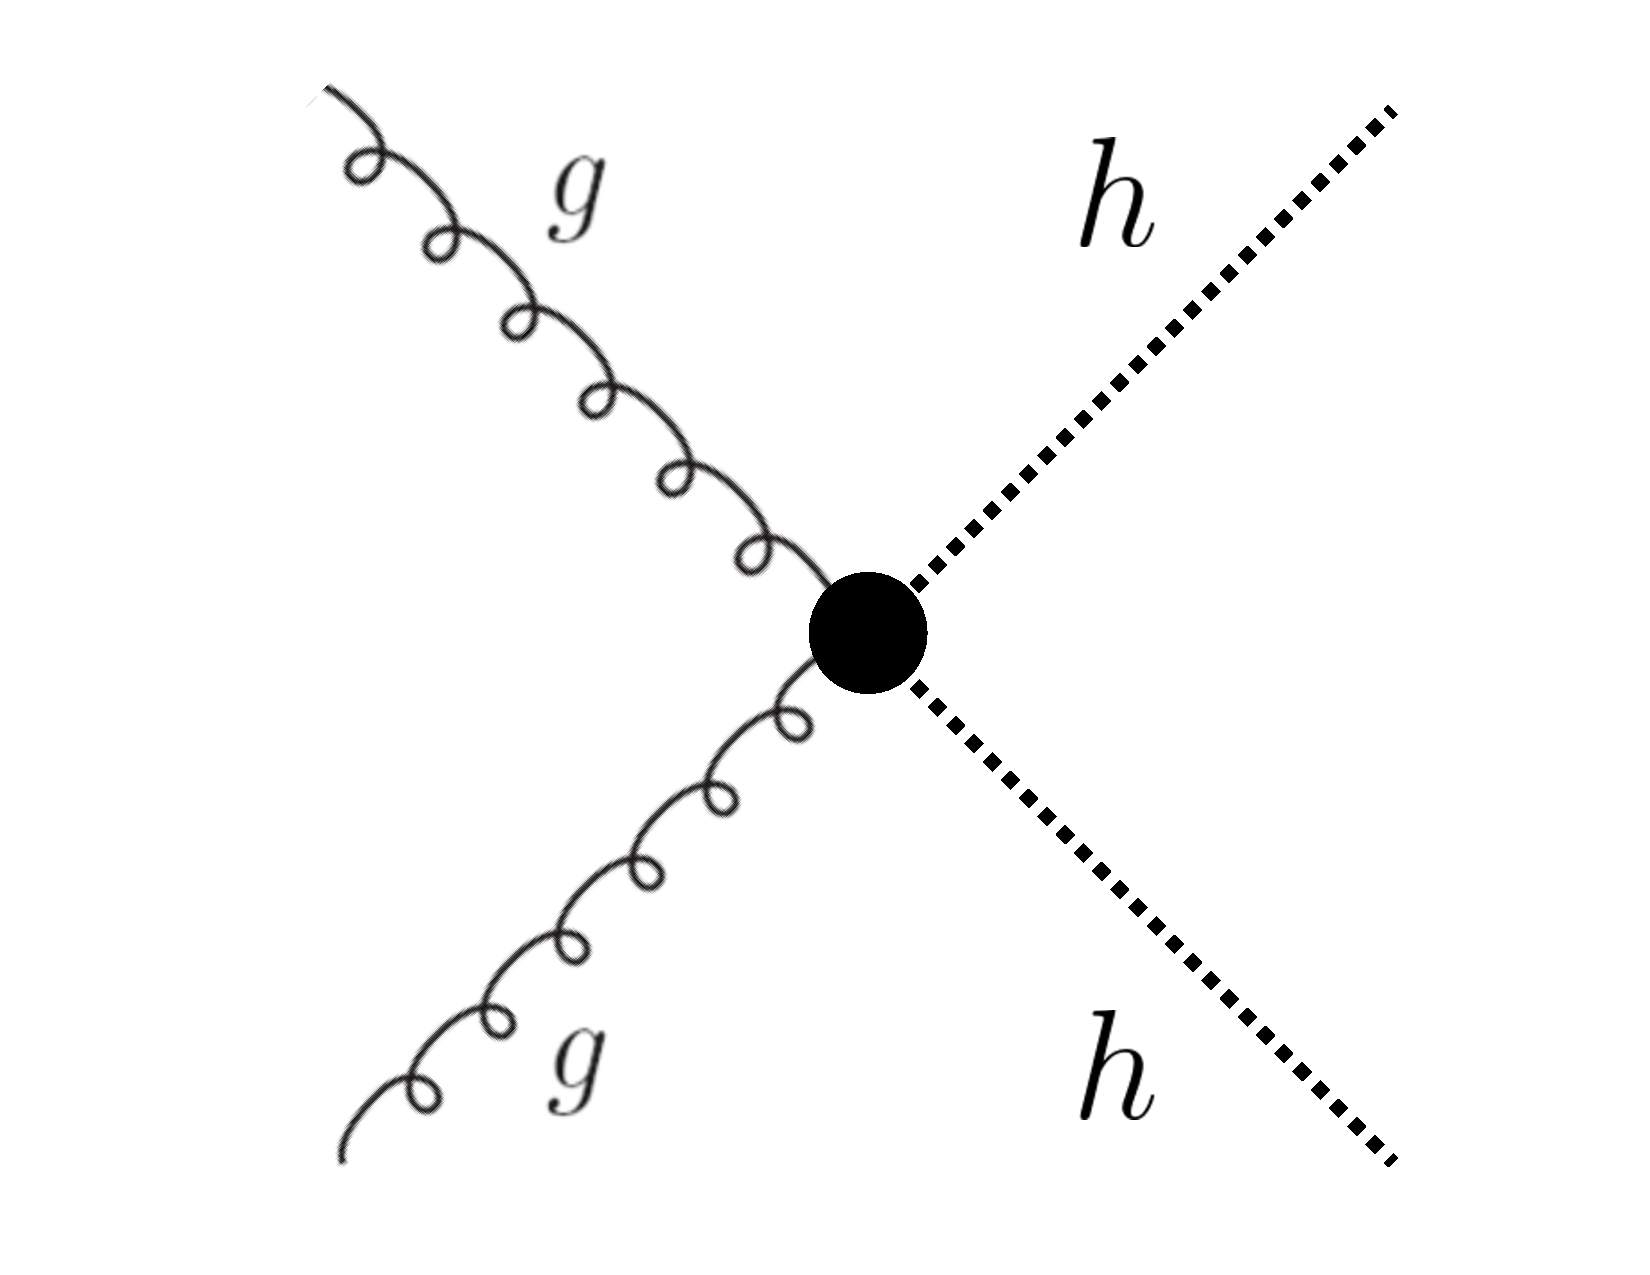
\includegraphics[width=0.4\textwidth]{figures/HH_nonres2}
   \caption{Diagrams with new vertices for non-resonant Higgs pair production arising in composite Higgs models}
  \label{fig:HH_nonres}
\end{figure}

The next sections provide more detail on the phenomenology of resonant Higgs production in Randall-Sundrum and 2HDM models, as these models will later be tested in a dedicated search for resonant production of boosted Higgs pairs. 

\begin{figure}[h!]
  %\vspace{20pt}
  \centering
  \captionsetup{justification=centering}

  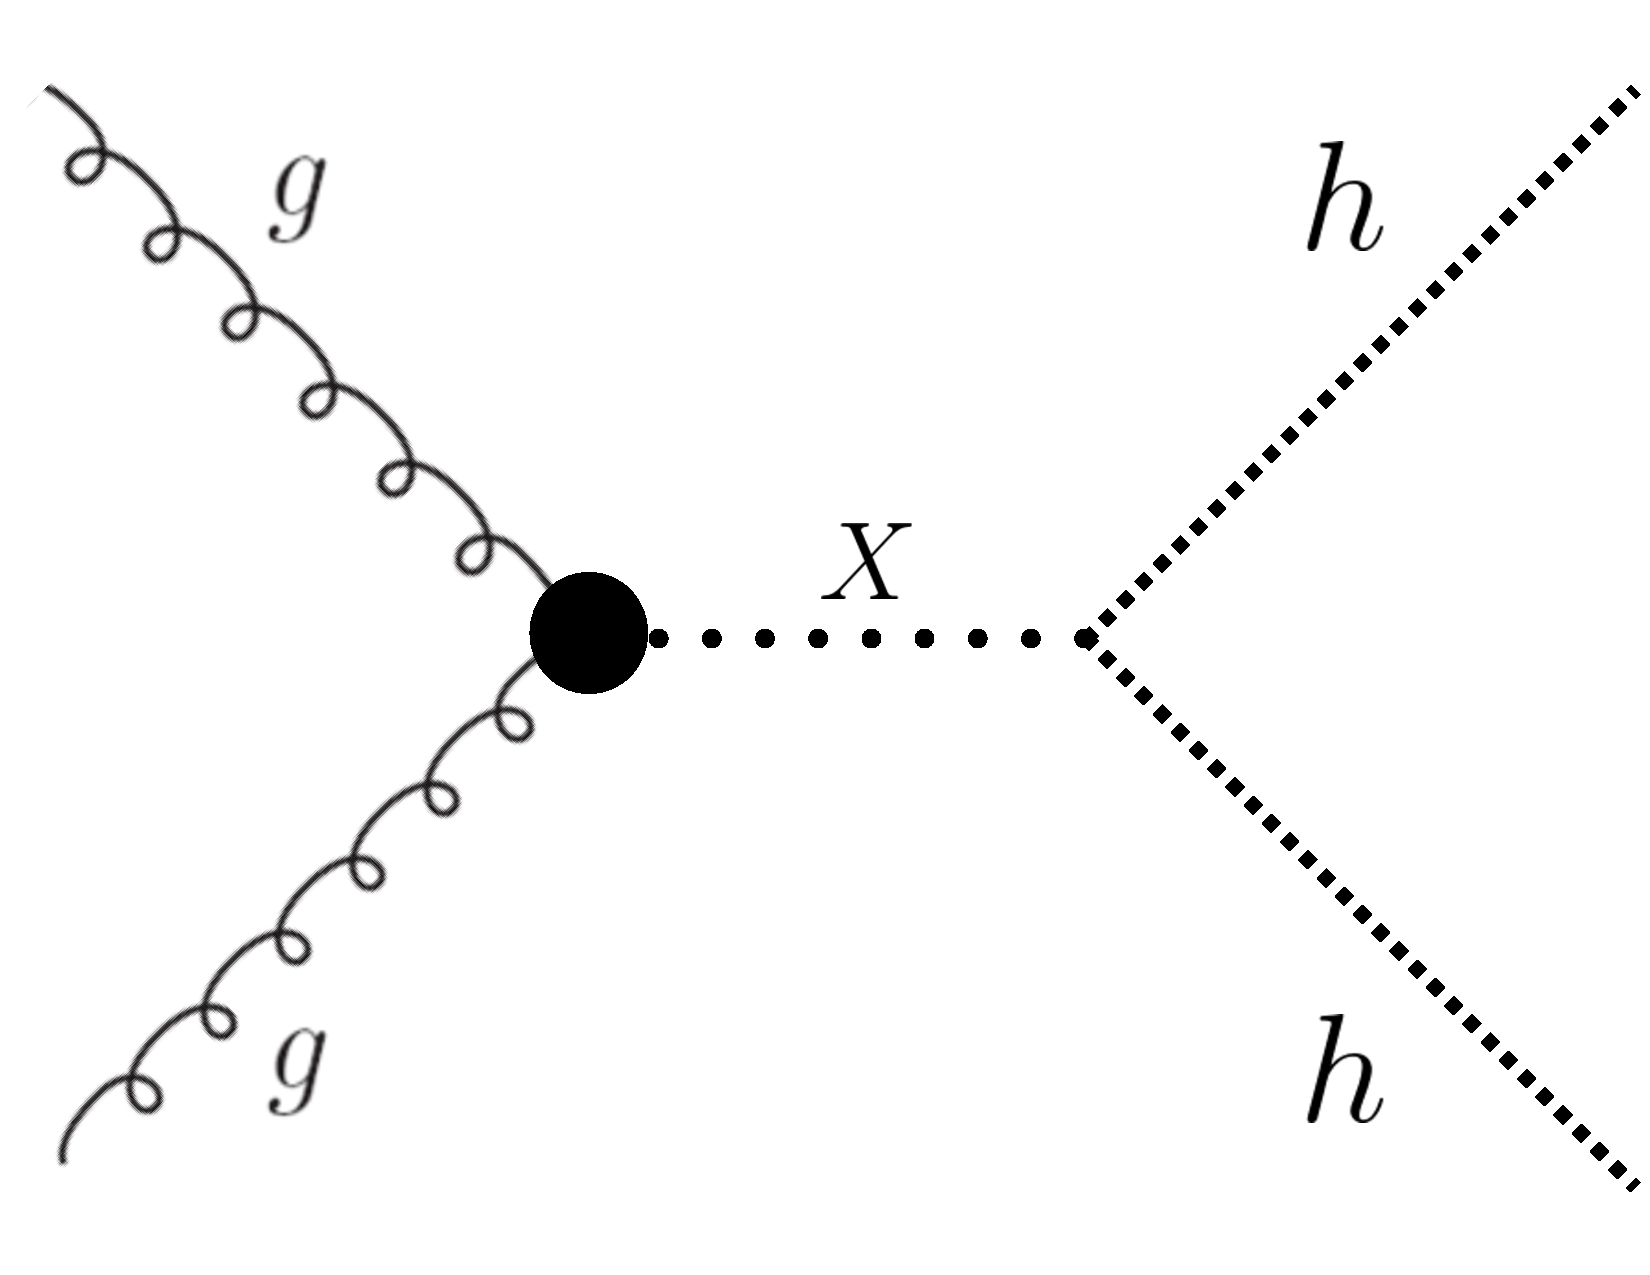
\includegraphics[width=0.4\textwidth]{figures/Generic_res}
   \caption{Generic Feynman diagram for resonant Higgs pair production in BSM theories}
  \label{fig:HH_res}
\end{figure}

\subsection{Randall-Sundrum Gravitons}

The Randall-Sundrum model is a proposed solution to the hierarchy problem that posits a five-dimensional warped spacetime that contains two branes: one where the force of gravity is very strong and a second brane at the $\TeV$ scale corresponding to the known Standard Model sector~\cite{RSG1}. In the theory, the branes are weakly coupled and the graviton probability function drops exponentially going from the gravity brane to the SM brane, rendering gravity weak on the SM brane. The experimental consequence of this theory is a tower of widely spaced (in mass) Kaluza-Klein graviton resonances. In theories where the fermions are localized to the SM brane, production of gravitons from fermion pairs is suppressed and the primary mode of production is gluon fusion\cite{RSG_LHC}. These gravitons have a substantial branching fraction to Higgs pairs, ranging from $6.43$\% for gravitons with a mass of $500 \GeV$ to $7.66\%$ at $3 \TeV$. Figure~\ref{fig:G_BR} shows the branching ratios of the spin-2 Randall Sundrum graviton (RSG) as a function of its mass. The predominant decays are to $t\bar{t}$ above the mass threshold for that channel. 


\begin{figure}[h!]
  %\vspace{20pt}
  \centering
  \captionsetup{justification=centering}

  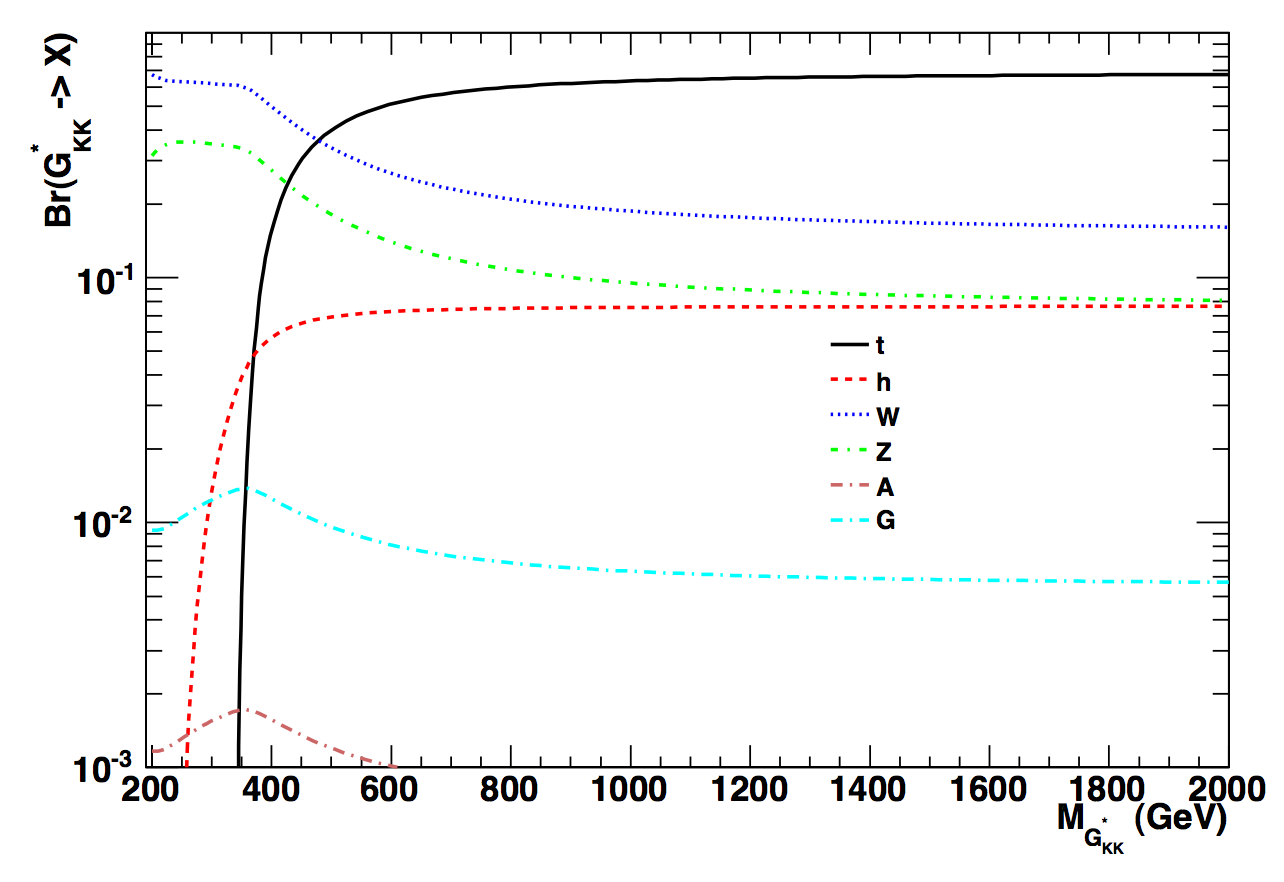
\includegraphics[width=0.7\textwidth]{figures/G_BR}
   \caption{Branching ratios for a spin-2 Randall-Sundrum graviton as a function of mass computed in MadGraph with the CP3-Origins implementation~\cite{RSG_LHC,MadGraph}}
  \label{fig:G_BR}
\end{figure}

These models have two free parameters - the mass of the graviton and a curvature parameter $k$. Typically, rather than $k$, the theory is parameterized using $c \equiv k/\bar{M_{\rm pl}}$, where $\bar{M_{\rm pl}}$ is the reduced Planck mass. The cross section for production of the RSG decreases as a function of mass and is strongly dependent on the gluon PDF. The increase in center of mass energy from $8$ to $13 \TeV$ in LHC Run 2 greatly increases the cross section at higher mass. Figure~\ref{fig:G_xsec} shows the cross section as a function of graviton mass at $\sqrt{s} = 13 \TeV$ for RSG models with $c=1.0$ and $c=2.0$. 

\begin{figure}[h!]
  %\vspace{20pt}
  \centering
  \captionsetup{justification=centering}

  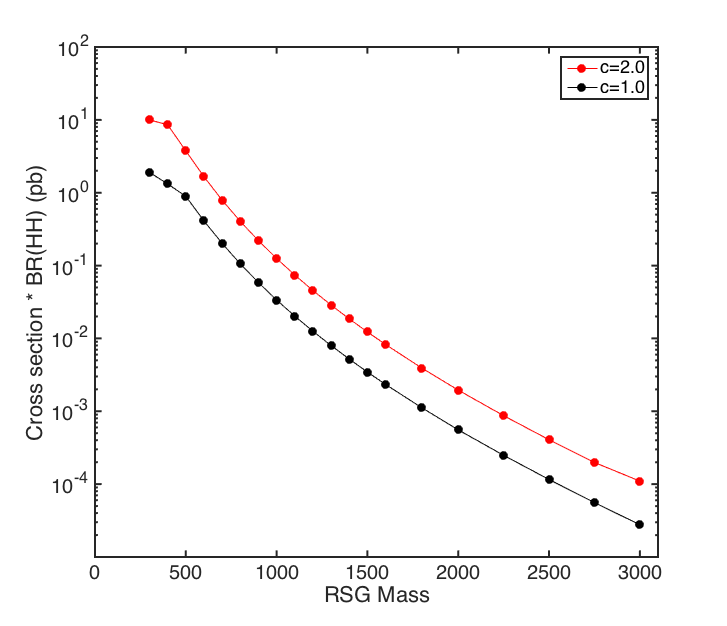
\includegraphics[width=0.7\textwidth]{figures/RSG_xsec}
   \caption{$\sigma \times \textrm{BR}(HH)$ for RSG as a function of mass computed in MadGraph with the CP3-Origins implementation~\cite{RSG_LHC,MadGraph}}
  \label{fig:G_xsec}
\end{figure}

Another interesting feature of the theory is that the width of the graviton increases with both $c$ and $m_G$. Figure~\ref{fig:G_width} shows the graviton width for both $c=1.0$ and $c=2.0$ as a function of mass. In $c=1.0$, the width starts at $8.365 \GeV$ for a mass of $300 \GeV$ and increases to $187.2 \GeV$ at a mass of $3 \TeV$. SImilarly, with $c=2.0$, the width starts at $33.46 \GeV$ for $m_G = 300 \GeV$ and increases to $748.8 \GeV$ at a mass of $3 \TeV$. 


\begin{figure}[h!]
  %\vspace{20pt}
  \centering
  \captionsetup{justification=centering}

  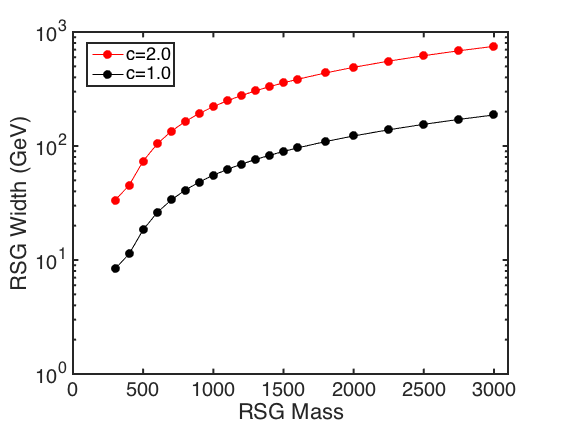
\includegraphics[width=0.7\textwidth]{figures/RSG_width}
   \caption{RSG width as a function of mass computed in MadGraph with the CP3-Origins implementation~\cite{RSG_LHC,MadGraph}}
  \label{fig:G_width}
\end{figure}



% For an example of a full page figure, see Fig.~\ref{fig:myFullPageFigure}.

%\texttt{This is a line of code.}

%\begin{figure}
%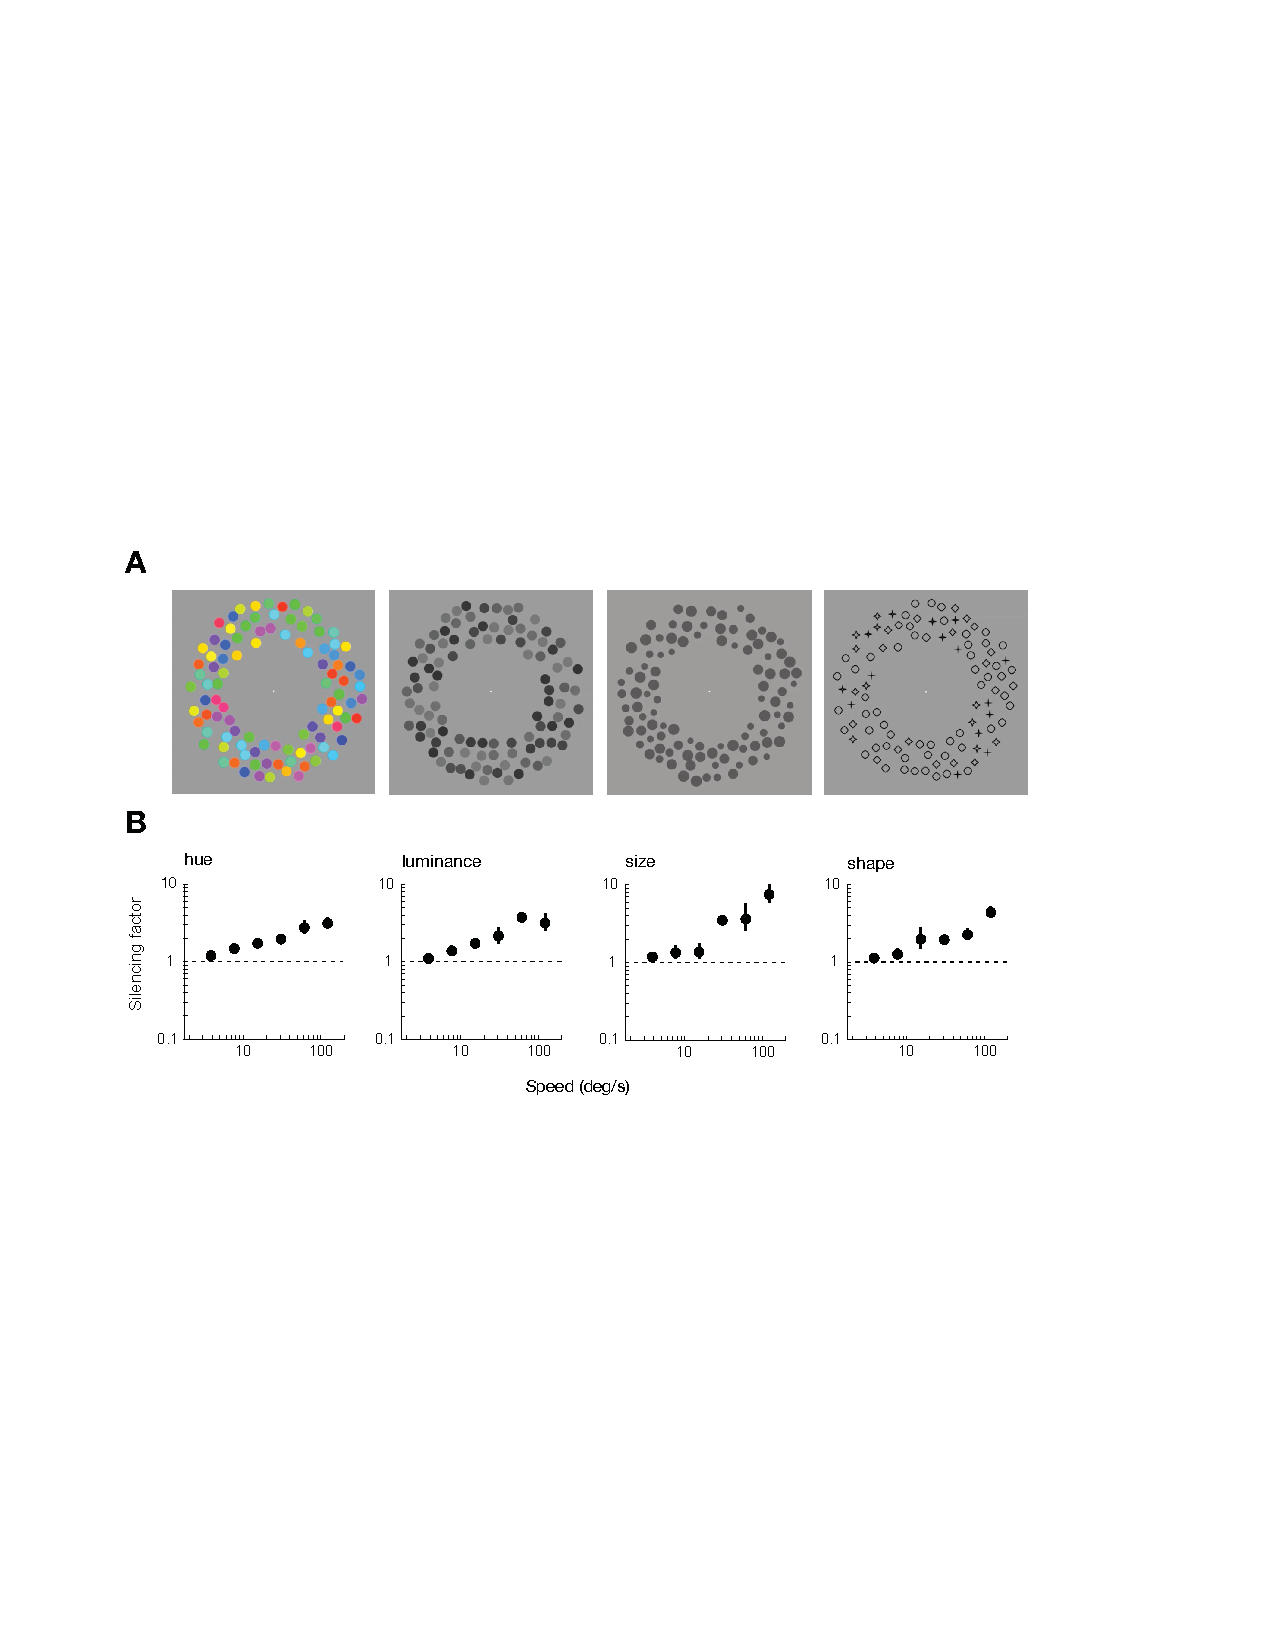
\includegraphics[width=\textwidth]{figures/fig1}
%\caption[Short figure name.]{This is a figure that floats inline and here is its caption.
%\label{fig:myInlineFigure}}
%\end{figure}

%% Requires fltpage2 package
%%
% \begin{FPfigure}
% 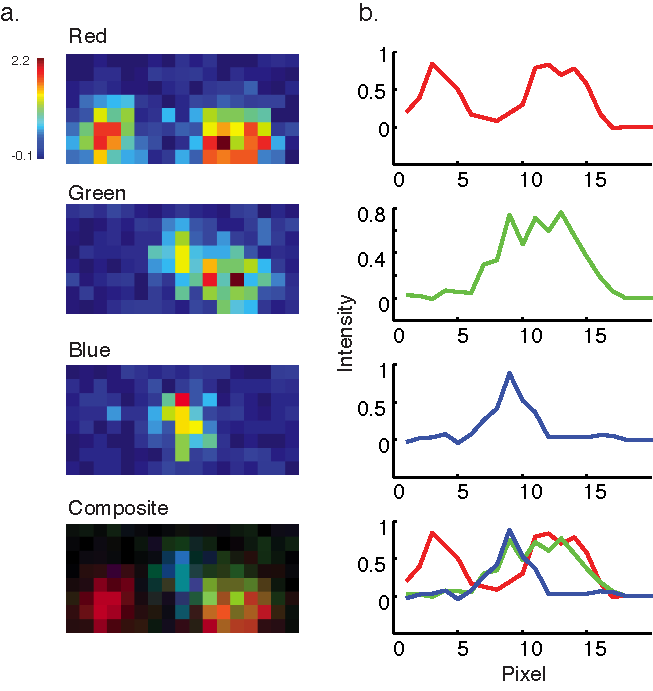
\includegraphics[width=\textwidth]{figures/fullpage}
% \caption[Short figure name.]{This is a full page figure using the FPfigure command. It takes up the whole page and the caption appears on the preceding page. Its useful for large figures. Harvard's rules about full page figures are tricky, but you don't have to worry about it because we took care of it for you. For example, the full figure is supposed to have a title in the same style as the caption but without the actual caption. The caption is supposed to appear alone on the preceding page with no other text. You do't have to worry about any of that. We have modified the fltpage package to make it work. This is a lengthy caption and it clearly would not fit on the same page as the figure. Note that you should only use the FPfigure command in instances where the figure really is too large. If the figure is small enough to fit by the caption than it does not produce the desired effect. Good luck with your thesis. I have to keep writing this to make the caption really long. LaTex is a lot of fun. You will enjoy working with it. Good luck on your post doctoral life! I am looking forward to mine. \label{fig:myFullPageFigure}}
% \end{FPfigure}
% \afterpage{\clearpage}



\begin{savequote}[75mm]
This is some random quote to start off the chapter.
\qauthor{Firstname lastname}
\end{savequote}

\chapter{The ATLAS detector and the Large Hadron Collider}

This chapter presents an overview of the experimental systems used to conduct the measurements presented in this thesis. First, a brief overview of the accelerator, the Large Hadron Collider, will be given. In this section, the accelerator conditions relevant to data-taking are presented as well. Next, an overview of the ATLAS experiment is given. The basics of each sub-detector's role are summarized, as well as the details of the datasets accumulated. Then, a brief interlude on the ATLAS Muon New Small Wheel upgrade is presented. While this new detector does not have a direct impact on any of the datasets taken so far, it will have an impact on future analyses and the work done on it is briefly summarized here. Finally, an overview of object reconstruction in ATLAS is given. While the details of all of the algorithms will not be presented in detail, aspects of the reconstruction performance such as object resolutions are shown as these are relevant to the two studies presented later in this thesis. 

\section{The Large Hadron Collider}

The Large Hadron Collider (LHC) is a proton-proton collider at the CERN laboratory in Geneva, Switzerland\cite{LHCPaper}. It is designed for a maximum collision center of mass energy of $\sqrt{s} = 14 \TeV$ and has a circumference of $26.7$ kilometers. Four main experiments are located at the interaction points (IP) of the accelerator: ATLAS (A Toroidal LHC ApparatuS), CMS (the Compact Muon Solenoid), ALICE (A Large Ion Collider Experiment), and LHC$b$~\cite{ATLASPaper, CMSPaper, LHCbPaper, ALICEPaper}. The studies performed in this thesis were all completed with the ATLAS detector.

Figure~\ref{fig:LHC} shows a schematic of the LHC ring and the various experiments.  

\begin{figure}[h!]
  %\vspace{20pt}
  \centering
  \captionsetup{justification=centering}

  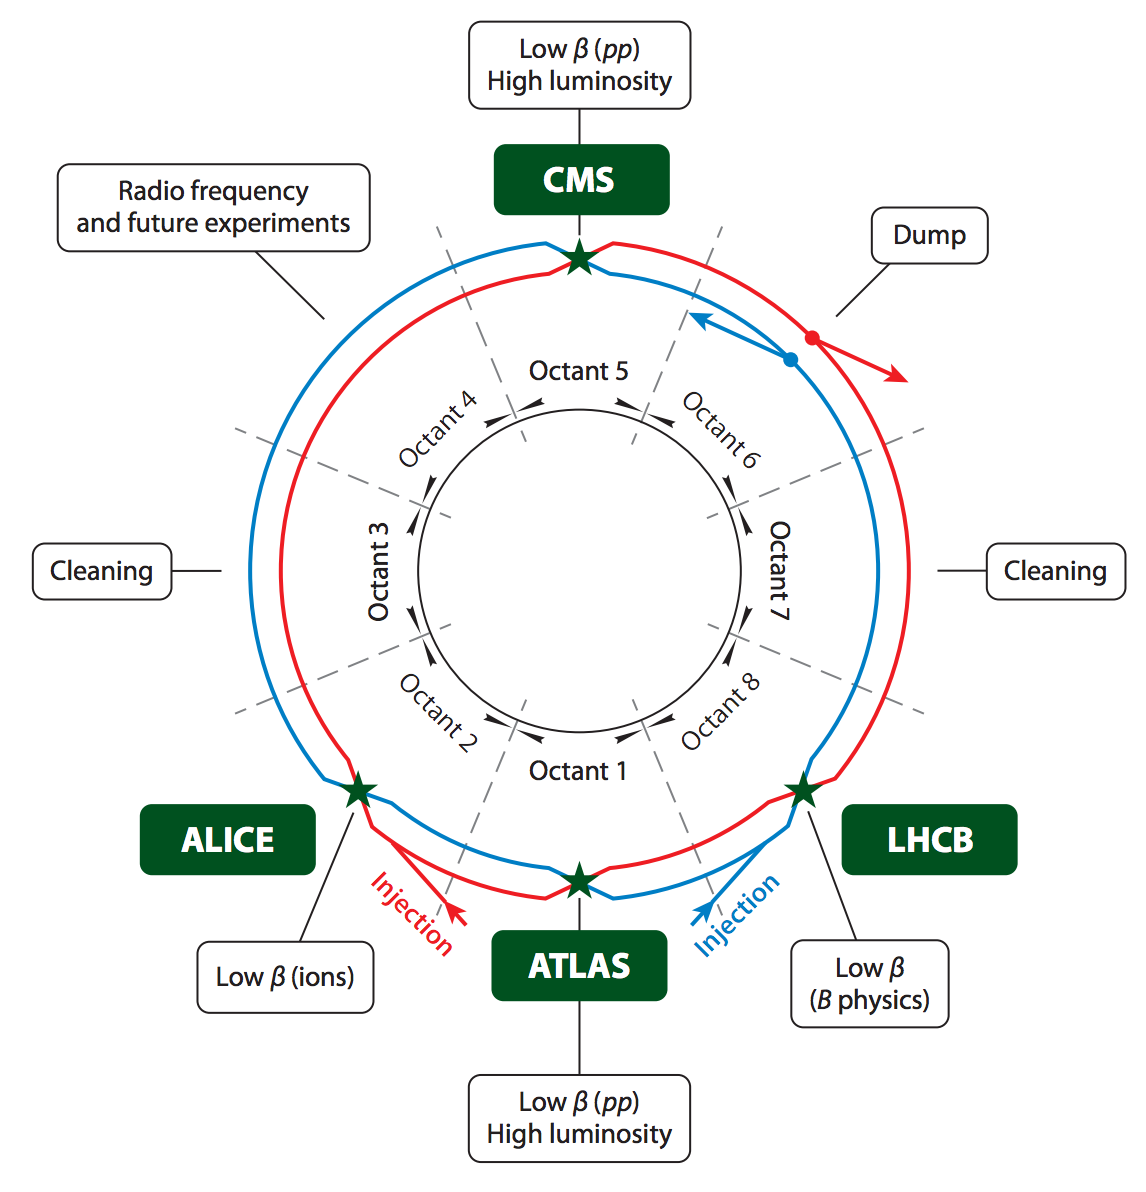
\includegraphics[width=0.7\textwidth]{figures/LHC}
   \caption{A schematic view of the LHC ring ~\cite{LHCReview}}
  \label{fig:LHC}
\end{figure}

One of the most interesting features of the LHC is in its magnet design. Because the tunnel does not have room for separate superconducting magnets for each of the beam pipes, the LHC employs a twin-bore magnet design. Each magnet must hold an $8.3$ Tesla magnetic field in order to bend the proton beams at $\sqrt{s} = 14 \TeV$. The superconducting magnets are cooled to a temperature of $1.9$ Kelvin with superfluid helium.  

\subsection{Instantaneous luminosity}

The rate of physics events expected from the accelerator is dependent on the instantaneous luminosity of the machine and the cross section of the physics process, $R_{\rm events} = L\sigma$. Here, $R_{\rm events}$ is the number of events per second, $L$ is the instantaneous luminosity of the machine, and $\sigma$ is the cross section for the physics process being measured. The instantaneous luminosity of the LHC is determined by numerous factors related to machine conditions. Equation~\ref{eqn:lumi} gives the equation for instantaneous luminosity of Gaussian beam profile~\cite{LHCReview}.

\begin{equation}
\label{eqn:lumi}
L = \frac{N_b^2 n_b f_{\rm rev} \gamma_r}{4\pi \epsilon_n \beta^*} F
\end{equation}

The LHC collides protons in bunches, and in the above equation $N_b$ is the number of protons per bunch while $n_b$ is the number of bunches per beam. Nominally, the LHC can hold up to $2808$ proton bunches. $f_{\rm rev}$ is the revolution frequency. $\epsilon_n$ is the normalized transverse beam emittance, a measurement of the average spread of the particles position-momentum space which has the dimension of length. $\beta^*$ is the value of the $beta$ function for the beam at the interaction point. It relates the emmitance to the Gaussian width of the beam with $\sigma_{\rm beam} = \sqrt{\epsilon \cdot \beta}$. $F$ is a reduction factor that corrects for the fact that the beams are colliding at an angle at the IP. 

Another way of writing the instantaneous luminosity is shown in equation~\ref{eqn:lumi2}. In this case, the instantaneous luminosity is written as the ratio of the rate of inelastic collisions with the inelastic cross section\cite{lumi-paper}. 

\begin{equation}
\label{eqn:lumi2}
L = \frac{R_{\rm inel}}{\sigma_{\rm inel}} = \frac{\mu n_b f_{\rm rev}}{\sigma_{\rm inel}}
\end{equation}

In this case, $\mu$ is the average number of interactions per bunch crossing in the accelerator. $\mu$ is a useful parameter for characterizing the amount of activity recorded in an experiment. As the instantaneous luminosity and thus $\mu$ increase, there are more interactions per bunch crossing and more activity in the detector. This is often characterized with $\langle \mu \rangle$, the measured per bunch crossing $\mu$ value averaged over all bunch crossings. The interactions inside each bunch crossing that are not the main physics process of interest are often referred to as ``pileup" interactions, and $\langle \mu \rangle$ is a measurement of the level of pileup in the detector. 

\subsection{Evolution of machine conditions}

This thesis uses datasets taken at three different center of mass energies: $\sqrt{s} = 7 \TeV$ data taken in the year $2011$, $\sqrt{s} = 8 \TeV$ data taken in the year $2012$, and $\sqrt{s} = 13 \TeV$ dataa taken in the year $2015$. In addition to increasing center of mass energy, the instananeous luminosity and parameters that determine it were evolving. Table~\ref{tab:LHC_cond} summarizes that machine conditions in each of these datasets. 

\begin{table}[h!]
\centering
\captionsetup{justification=centering}

%\begin{tabular*}{0.480\textwidth}{p{0.075\textwidth} p{0.180\textwidth} l}
\hspace{-10pt}
\begin{tabular}{|c|c|c|c|c|}
\hline
& $2011$ & $2012$ & $2015$ & Design\\ \hline
$\sqrt{s}$ [$\TeV$] & $7$ & $8$ & $13$ & $14$ \\ \hline
Number of bunches & $1380$ & $1380$ & $1825$ & $2808$ \\ \hline
Max. protons per bunch & $1.45\times10^{11}$ & $1.7\times10^{11}$ & & $1.15 \times 10^{11}$ \\ \hline
Bunch spacing [$\textrm{ns}$] & $50$ & $50$ & $25$ & $25$ \\ \hline
\specialcell{Max. instantaneous \\ luminosity [$\textrm{cm}^{-2} \textrm{s}^-1$]} & $3.7\times 10^{33}$ & $7.7\times10^{33}$ & $5\times10^{33}$ & $10^{34}$\\ \hline
$\beta^*$ [$\textrm{m}$] & $1.0$ & $0.6$ & $0.8$ & $0.55$ \\ \hline 
$\langle \mu \rangle$ & $11.6$ & $20.7$ & $13.7$ & - \\ \hline
\end{tabular}

\caption{
Evolution of LHC machine conditions~\cite{LHC_2011_2012,LHC_2015}
}
\label{tab:LHC_cond}
\end{table}


\section{The ATLAS Detector}

The ATLAS detector is a multi-purpose particle detector experiment at the LHC's Point $1$~\cite{ATLASPaper}. It has nearly $4\pi$ coverage in solid angle around the interaction point. It consists of an inner detector for measuring charged particles, electromagnetic and hadronic calorimeters, and a muon spectrometer. Figure~\ref{fig:ATLAS_overview} gives an overview of the detector.

\begin{figure}[h!]
  %\vspace{20pt}
  \centering
  \captionsetup{justification=centering}

  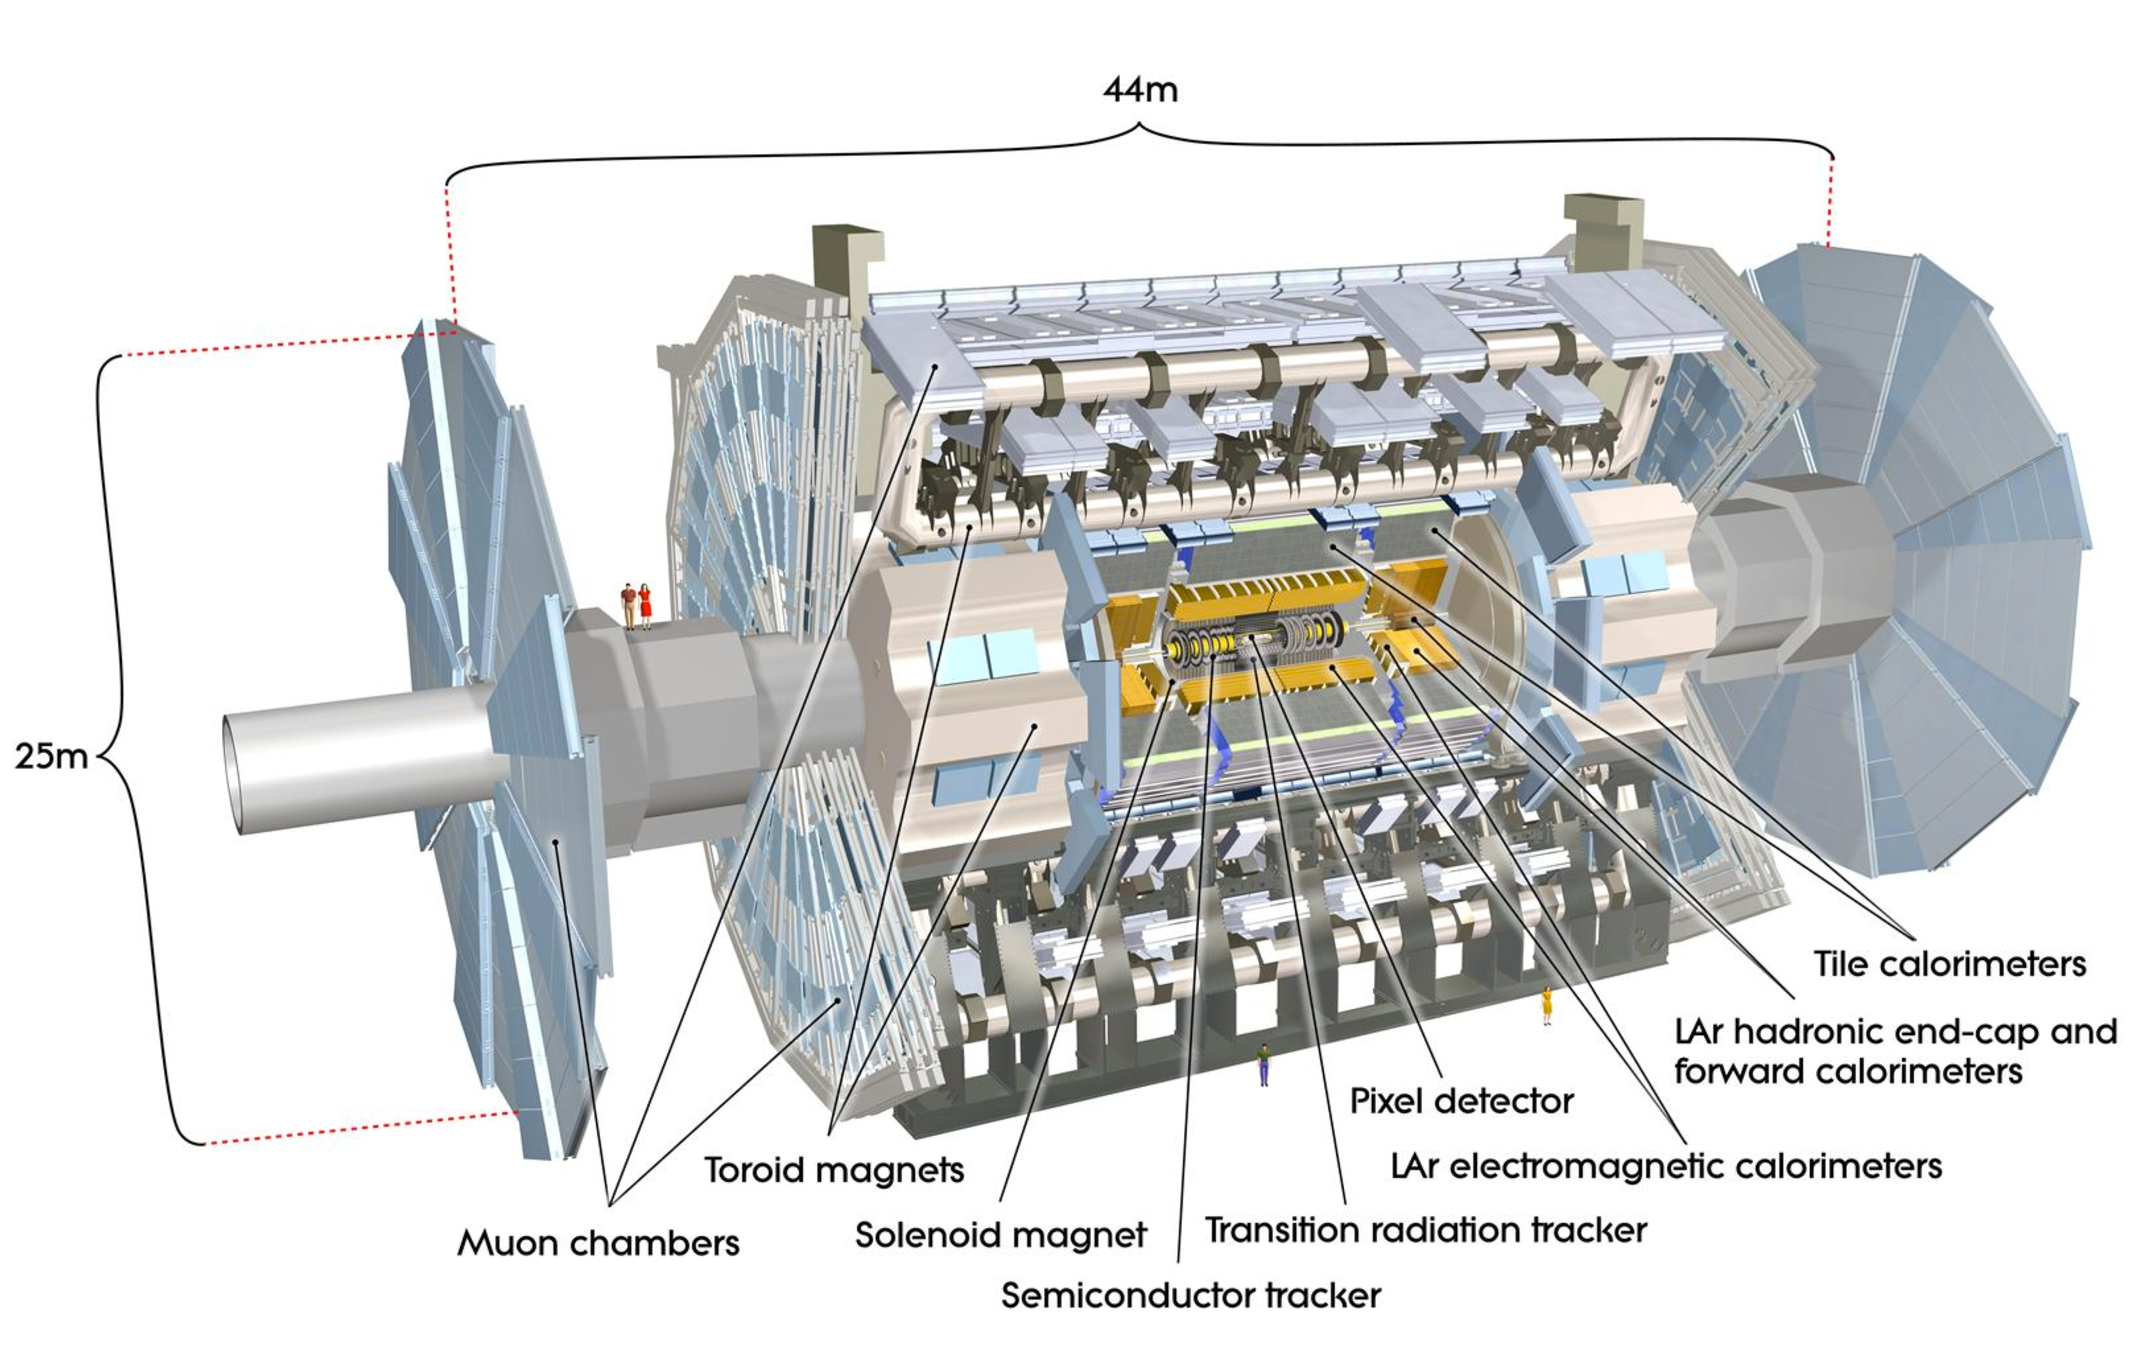
\includegraphics[width=\textwidth]{figures/ATLAS}
   \caption{A full diagram of the ATLAS detector~\cite{ATLASPaper}}
  \label{fig:ATLAS_overview}
\end{figure}

\subsection{Coordinate system}

Before defining the properties of the individual detectors, it is important to establish the coordinate system used. Figure~\ref{fig:coord} shows a schematic of the coordinate system. The azimuthal plane (perpendicular to the beam line) is defined as the $x$-$y$ plane. The angle in this plane is referred to as $\phi$. The angle relative to the beam axis is referred to as $\theta$. Rather than using $\theta$ directly as a coordinate, the experiment often uses the pseudorapidity $\eta$. $\eta$ is defined in equation~\ref{eqn:eta}. 

\begin{equation}
\label{eqn:eta}
\eta = \ln{\left(\tan\left(\frac{\theta}{2}\right)\right)}
\end{equation}

Pseudorapidity is the massless approximation of rapidity, the angle used to paramaterize boosts in special relativity. This is important for two reasons. First, it means that differences in $\eta$ are Lorentz invariant. Second, particle production is roughly constant in pseudorapidity. Particles with $\eta$ close to zero are referred to as ``central", while those at high $|\eta|$ are called ``forward". In general, two main detector topologies can be seen in figure~\ref{fig:ATLAS_overview}. There are ``barrel" elements, which surround the beam line cylindrically and are in the central region of the detector. In the forward region, there are ``endcap" regions which are arranged as disks perpendicular to the beam line. 

\begin{figure}[h!]
  %\vspace{20pt}
  \centering
  \captionsetup{justification=centering}

  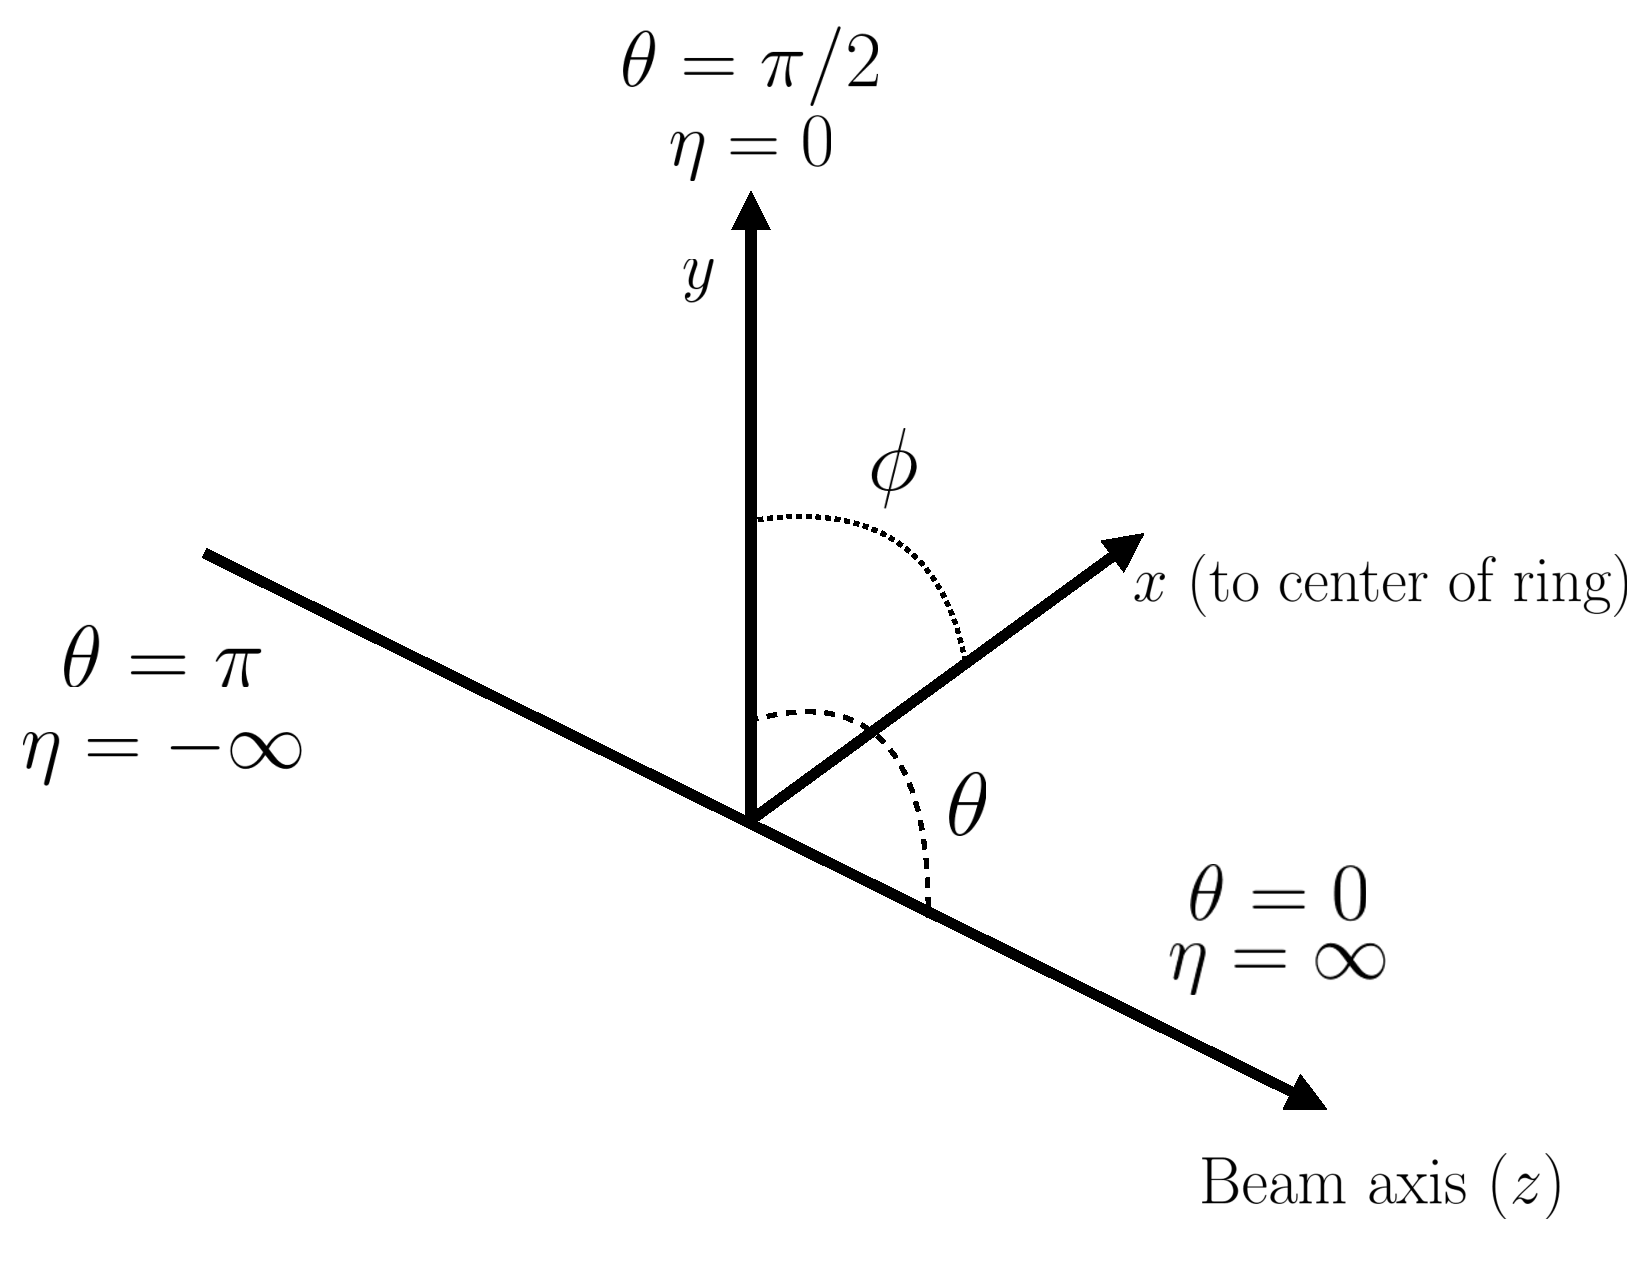
\includegraphics[width=0.8\textwidth]{figures/ATLAS_coord}
   \caption{The ATLAS coordinate system}
  \label{fig:coord}
\end{figure}

\subsection{Inner detector}

The ATLAS Inner Detector (ID) system is built for precision tracking of charged particles. It covers the range $|\eta| < 2.5$. In this range, approximately $1000$ particles are generated every bunch crossing in the detector. This requires having fine granularity to achieve the resolutions required for good momentum measurement and vertex reconstruction. 

The ID consists of three sub-components: the pixel detector, semiconductor tracker (SCT), and transition radiation tracker (TRT). It is surrounded by a solenoid providing a $2$ $\rm T$ axial magnetic field which bends particles in the transverse plane to allow for momentum measurement. Figure~\ref{fig:ID}shows the layout of each of these components. 

\begin{figure}[h!]
  %\vspace{20pt}
  \centering
  \captionsetup{justification=centering}

  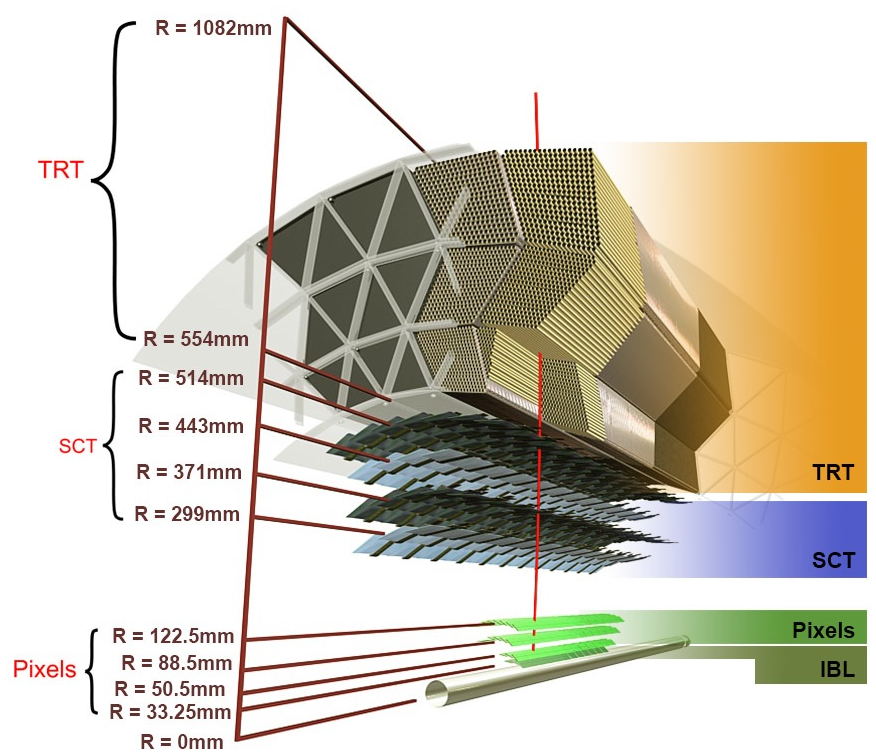
\includegraphics[width=0.7\textwidth]{figures/ATLAS_ID}
   \caption{Layout of the ATLAS Inner Detector system~\cite{Run2Tracking}}
  \label{fig:ID}
\end{figure}

\subsubsection{Pixel detector}

The pixel detector is the first detector particles traverse after being generated in proton collisions and is the most granular detector. Its operation is crucial for precision tracking and vertex reconstruction as well as higher level object reconstruction like tagging of jets from $b$-quarks. The basic sensing element in this subdetector is a silicon pixel detector. The operating principle for the silicon pixels is that of a $p$-$n$ junction. When a charged particle passes through, it creates electron-hole pairs that are then separated by the electric field. The sensors are $250\,\mu\rm m$ thick and use oxygenated $n$-type wafers with readout pixels on the $n^+$ side of the detector~\cite{ATLASPaper}. Overall, the pixel detector has $1744$ sensors and $~80.4$ million readout channels.

In the barrel region, the pixel detector has three concentric layers of sensors surrounding the beamline. In the endcap region, it consists of disks perpendicular to the beam axis. The detector is segmented in the $R$-$\phi$ plane and in $z$. Usually, three pixel layers are crossed by a charged particle track. The intrinsic accuracies of the sensors are $10\,\mu\rm m$ in $R$-$\phi$ and $115\,\mu\rm m$ in $z$ (or $R$ for the endcap).


\subsubsection{Insertable B-layer}

In Run 2, a new innermost pixel layer, known as the insertable B-layer (IBL), was added to the Inner Detector~\cite{IBL}. This layer was added to cope with the higher luminosities planned in LHC Run 2 and at the high luminosity HL-LHC. Additionaly it improves tracking position resolution which in turn improves the vertexing and $b$-tagging capabilities in ATLAS. The detector sits directly on a new beam pipe, only $33.25 \textrm{ mm}$ away from the collision points in the azimuthal plane. 

\subsubsection{Semiconductor Tracker (SCT)}

The semiconductor tracker (SCT) consists of silicon microstrips and comprises the next four layers of the ID. This sub-detector has $6.4 \textrm{cm}$ long sensors that are daisy-chained into strips with a strip pich of $80 \,\mu\rm m$~\cite{ATLASPaper}. Some of the strips have a small stereo angle to allow for measurement of both angular coordinates. In total there are $6.3$ million readout channels. The intrinsic accuracies are $17 \,\mu\rm m$ in $R$-$\phi$ and $580 \,\mu\rm m$ in $z$ (or $R$ in the endcap).

\subsubsection{Transition radiation tracker (TRT)}

The transition radiation tracker (TRT) serves two purposes. First, it consists of $4 \rm mm$ diameter straw tubes filled with a $70/27/3$\% gas mixture of xenon, carbon dioxide, and oxygen to provide tracking of charged particles. Particles typically have $36$ TRT straw tube hits per track. The material in between the straws is designed to induce transition radiation which can be useful for particle identification. As particles pass between media with different dielectric constants, they emit transition radiation that can cause additional showers in the TRT. In particular it is useful for discrimination between electrons and pions or other charged hadrons, as the amount of transition radiation is proportional to the Lorentz factor of the particle.

\subsection{Calorimeters}

The calorimeter system consists of two main sub-components: a fine granularity electromagnetic calorimeter tailored for the measurement of photons and electrons and multiple coarser hadronic calorimeters dedicated to the measurement of hadronic showers~\cite{ATLASPaper}. The calorimeter system has broader coverage than the inner detector, covering the region out to $|\eta| < 4.9$. It is also designed to deliver good containment of showers so as to limit leakage into the muon system. Figure~\ref{fig:ATLAS_calo} shows the layout of the calorimeter system. 

Both the electromagnetic and hadronic calorimeters are sampling calorimeters. They alternate active material for energy measurement with passive material for energy absorption. The materials used for each purpose vary based on the type of calorimeter and its location in the detector. 

\begin{figure}[h!]
  %\vspace{20pt}
  \centering
  \captionsetup{justification=centering}

  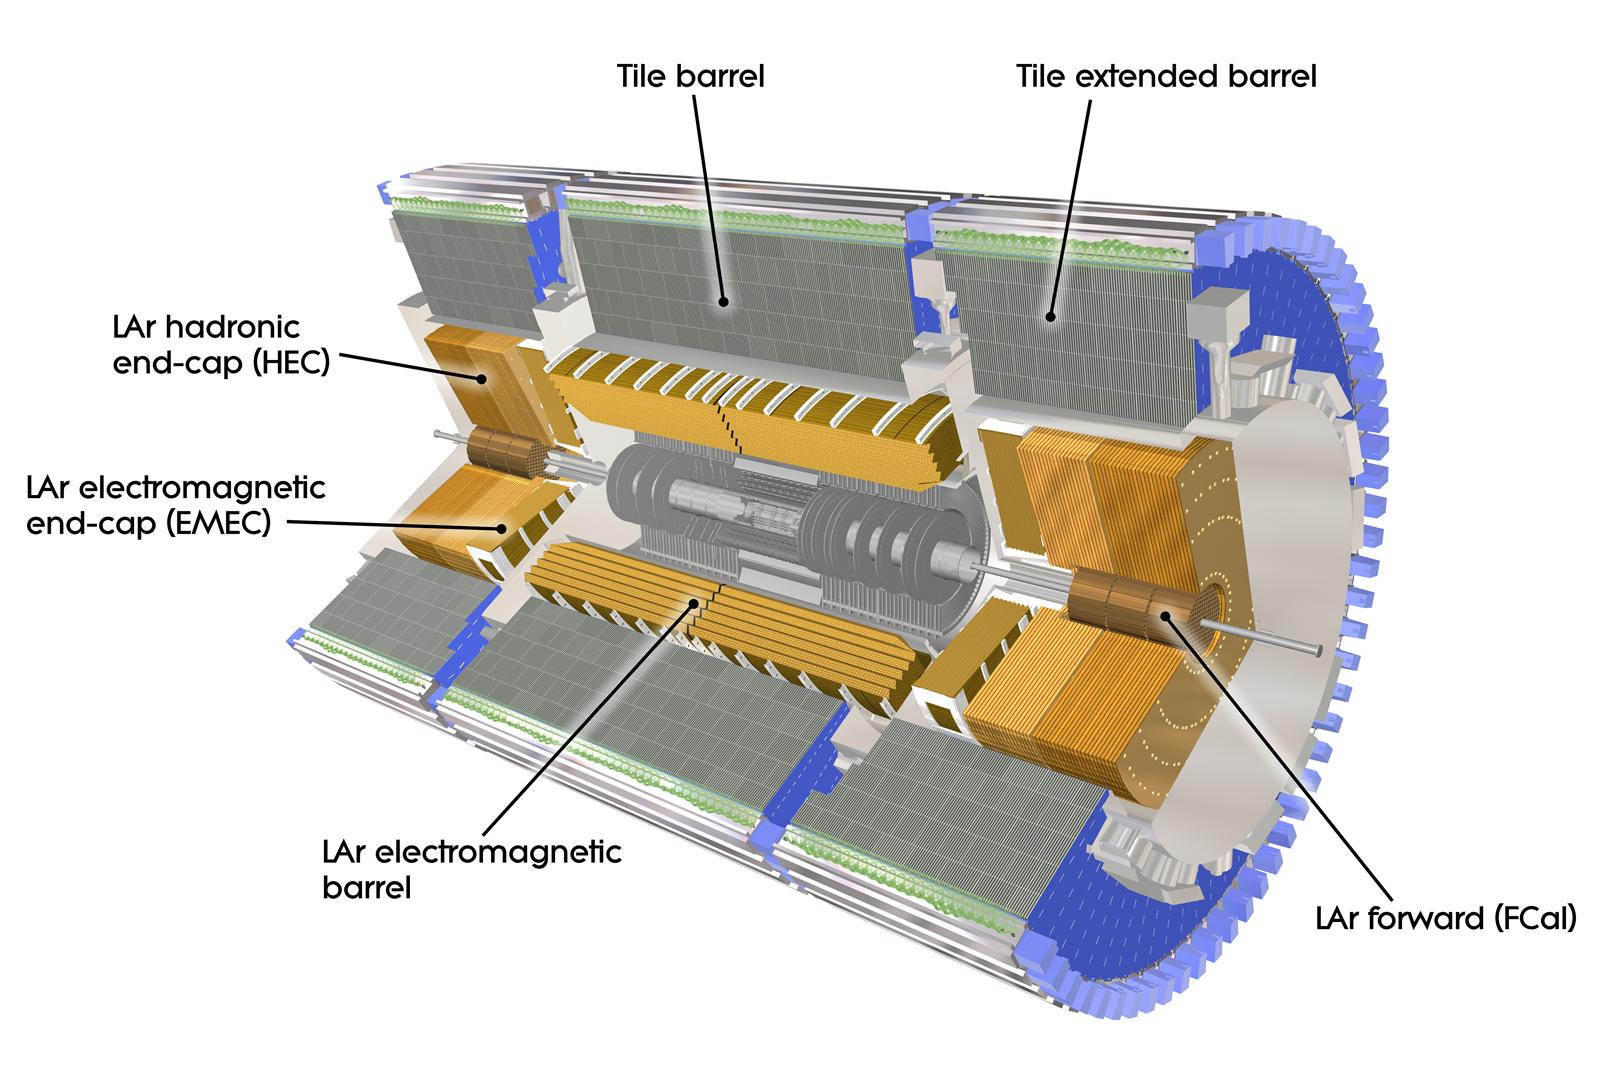
\includegraphics[width=\textwidth]{figures/ATLAS_calo}
   \caption{Layout of the ATLAS calorimeter system~\cite{ATLASPaper}}
  \label{fig:ATLAS_calo}
\end{figure}

\subsubsection{Electromagnetic calorimeter}

The electromagnetic calorimeter (EM calorimeter) use liquid Argon (LAr) as its active material and lead as its passive material. It is arrange in an accordion geometry to increase the absorption area while still allowing it to have no azimuthal cracks (complete symmetry in $\phi$). The EM calorimeter is divided into a barrel portion that extends to $|\eta| < 1.475$ and an endcap portion going from $1.375 < |\eta| < 3.2$. The region where these two units overlap is called the ``transition region". 

In order to provide good containment the calorimeter depth must be optimized. Typically, for electromagnetic calorimeters the depth is meaasured in radiation lengths. In general, the intensity of a particle beam attenuates exponentially in distance with a constant equal to the radiation length. That is, $I(x) = I_0 e^{-x/X_0}$, where $I$ is the intensity, $x$ is the distance traveled, and $X_0$ is the radiation length. The ATLAS EM calorimeter is designed to have $>22$ radiation lengths in the barrel and $> 24$ in the endcap~\cite{ATLASPaper}. 

\subsubsection{Hadronic calorimeters}

There are three types of hadronic calorimeters present in ATLAS: the tile calorimeter (TileCal), hadronic endcap (HEC), and forward calorimeter (FCal). Each one is optimized for stopping of hadronic showers and the materials chosen are specific to their placement in the detector. 

The TileCal is a scintillating tile calorimeter placed directly outside the EM calorimeter. It uses steel as the absorber and plastic scintillator tiles as the active material. It has coverage in the barrel at $|\eta| < 1.0$ and in the ``extended barrel" region of $0.8 < |\eta| < 1.7$.

The HEC had two wheels perpendicular to the beam line per endcap and is located directly behind the EM calorimeter endcap modules. The HEC covers the region from $1.5 < |\eta| < 3.2$, overlapping slightly with both the tile calorimeter and the forward calorimeter. Like the EM calorimeter, it uses liquid Argon as the active material, but it uses copper as the absorber. 

The FCal covers the most forward regions of the calorimeter system, extending to the region of $3.1 < |\eta| < 4.9$. It again uses liquid argon as its active material. For absorber, it consists of an innermost module made of copper followed by a module made of tungsten. 

The hadronic equivalent of radiation length is called the interaction length and is denoted as $\lambda$. In the barrel, the hadronic calorimeter depth is approximately $9.7\lambda$, while in the endcap is is $10\lambda$. The outer supports contribute an additional $1.3\lambda$. This is been shown to be sufficient to limit punch-through of showers to the muon system~\cite{ATLASPaper}.

\subsection{Muon spectrometer}

The muon spectrometer is dedicated to measuring the momentum and position of muons. It consists of tracking and trigger chambers which are unique in the barrel and endcap regions. The magnetic field for bending of muons is provided by a system of three large air-core toroid magnets (from which ATLAS derives its name.) These magnets provide $1.5$ to $5.5 \textrm{ Tm}$ of bending power at $0<|\eta|<1.4$ and approximately $1$ to $7.5 \textrm{ Tm}$ in the endcap region of $1.6 < |\eta| < 2.7$. The entire muon system covers the range $0 < |\eta|< 2.7$. Monitored drift tubes (MDTs) are used for tracking in the barrel and the two outer layers of the endcap, while cathode strip chambers (CSCs) are used to provide tracking in the innermost endcap wheel. In the barrel, resistive plate chambers (RPCs) are used as trigger chambers while thin gap chambers (TGCs) are used in the endcap. Figure~\ref{fig:ATLAS_muon} shows the layout of the ATLAS muon system. The entire muon system is designed with the specification of providing a $10\%$ momentum resolution for a $1 \TeV$ muon. 


\begin{figure}[h!]
  %\vspace{20pt}
  \centering
  \captionsetup{justification=centering}

  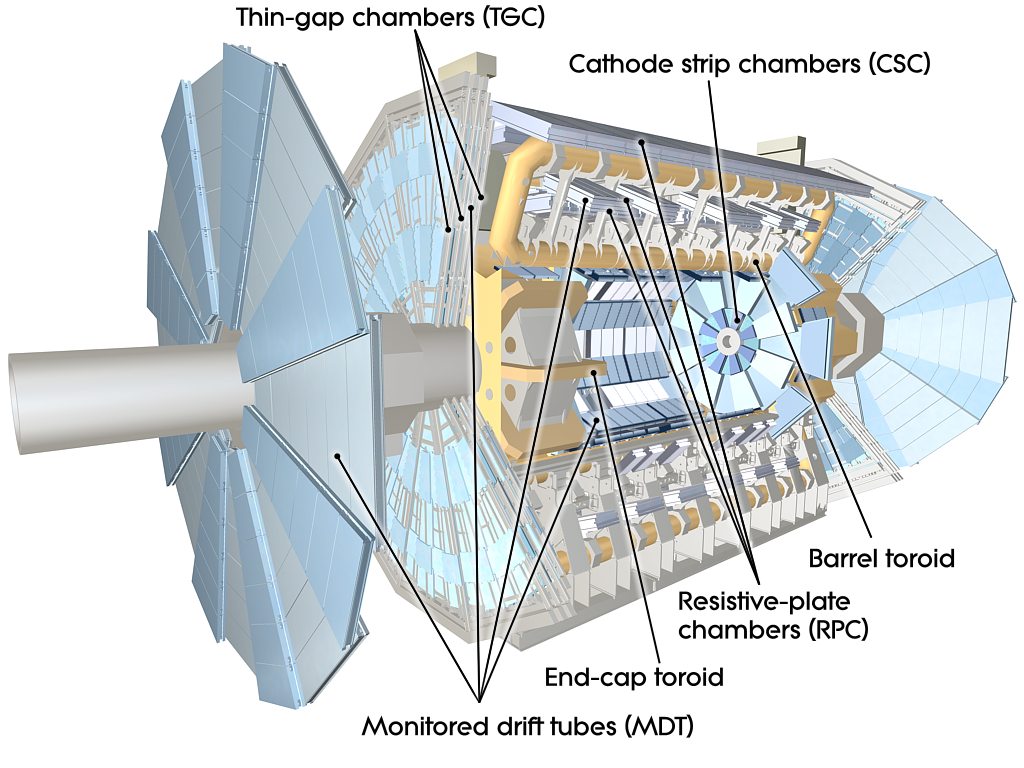
\includegraphics[width=0.9\textwidth]{figures/ATLAS_muon}
   \caption{Layout of the ATLAS muon system~\cite{ATLASPaper}}
  \label{fig:ATLAS_muon}
\end{figure}


\subsubsection{Monitored drift tubes (MDTs)}

The monitored drift tubes (MDTs) are aluminum $3 \rm cm$ diameter tubes filled with a $93/7$ \% mixture of Argon and $\textrm{CO}_2$, with trace amounts of water. As a charged particle traverses the tube, it ionizes the gas and the ions drift to a wire at the center of the tube. The radial distance of traversal of the particle in the tube is determined by the drift time of the electrons, allowing for fine position resolution. The tubes have an average resolution of $80\,\mu\textrm{m}$ per tube and a maximum drift time of approximately $700 \rm ns$. The tubes are oriented so that they give precision measurement in $\eta$ and run along $\phi$. They cover $|\eta| < 2.7$, except in the innermost layer of the endcap where they only go to $|\eta| < 2.0$~\cite{ATLASPaper}.

\subsubsection{Cathode strip chambers (CSCs)}

The cathode strip chambers cover a narrow window of the innermost endcap region at $2.0 < |\eta|< 2.7$. In this region the background rates in the cavern are particularly high and the CSCs are designed to handle these higher rates. The CSCs are multiwire proportional chambers with wires pointing in the radial direction (away from the beam pipe). The wire serves as an anode and there are two types of segmented cathode strip, one perpendicular to the wires which gives the precision measurement and one parallel which provides the transverse coordinate. It has an $80/20$ gas mixture of Argon and $\textrm{CO}_2$~\cite{ATLASPaper}. 

\subsubsection{Resistive plate chambers (RPCs)}

The resistive plate chambers (RPCs) are gaseous electrode-plate detectors covering the region $|\eta| < 1.05$. They consist of two resistive plates separated by a distance of $2\,\rm mm$. The gas mixture used is a $94.7/5/0.3$\% mixture of $\textrm{C}_2\textrm{H}_2\textrm{F}_4$, $\textrm{Iso-C}_4\textrm{H}_10$, and $\textrm{SF}_6$. It has readout strips with a pitch of $23$-$35\, \rm mm$ for both $\eta$ and $\phi$ measurement and thus provides measurement of the azimuthal coordinate in the barrel that the MDTs do not. The thin gas gap allows for a quick response time which makes it ideal for use in the trigger. There are three layers of RPCs which are referred to as the three trigger stations. They allwo for both a low $p_{T}$ and high $p_{T}$ trigger. The coincidence of hits in the innermost chambers allows for triggering of muons between $6$ and $9 \GeV$, while the outermost layer allows the trigger to select high momentum tracks in the range of $9$ to $35\GeV$~\cite{ATLASPaper}.

\subsubsection{Thin gap chambers (TGCs)}

The thin gap chambers (TGCs) are multiwire proportional chambers where the wire to cathode distance ($1.4\.\rm mm$) is smaller than the wire-to-wire distance ($1.8\,\rm mm$). They contain a gas mixture of $\textrm{CO}_2$ and $n$-pentane and use a hih electric field to gain good time resolution. They serve two functions in the end-cap system. First, they serve as the trigger chambers. Second, they also provide azimuthal coordinate measurement which the MDTs do not. They sit on the inner and middle layers of the endcap. The outermost layer's azimuthal coordinate is determined by extrapolation~\cite{ATLASPaper}.

\subsection{Magnet system}

As mentioned previously, there are two independent magnet systems in ATLAS. The first is a $2\,\rm T$ solenoid field in the inner detector which provides bending in the azimuthal plane. The second is an approximately $0.5\,\rm T$ toroidal field in the muon system which provides bending in $\eta$. Figure~\ref{fig:ATLAS_mag} shows the predicted field integral as a function of $|\eta|$~\cite{ATLASPaper}. 

\begin{figure}[h!]
  %\vspace{20pt}
  \centering
  \captionsetup{justification=centering}

   %\begin{subfigure}[t]{0.5\textwidth}
   %     \centering
   %     \includegraphics[width=0.7\textwidth]{figures/ATLAS_magnets}
   %     \caption{}
   % \end{subfigure}%
    %\begin{subfigure}[t]{0.5\textwidth}
    %    \centering
        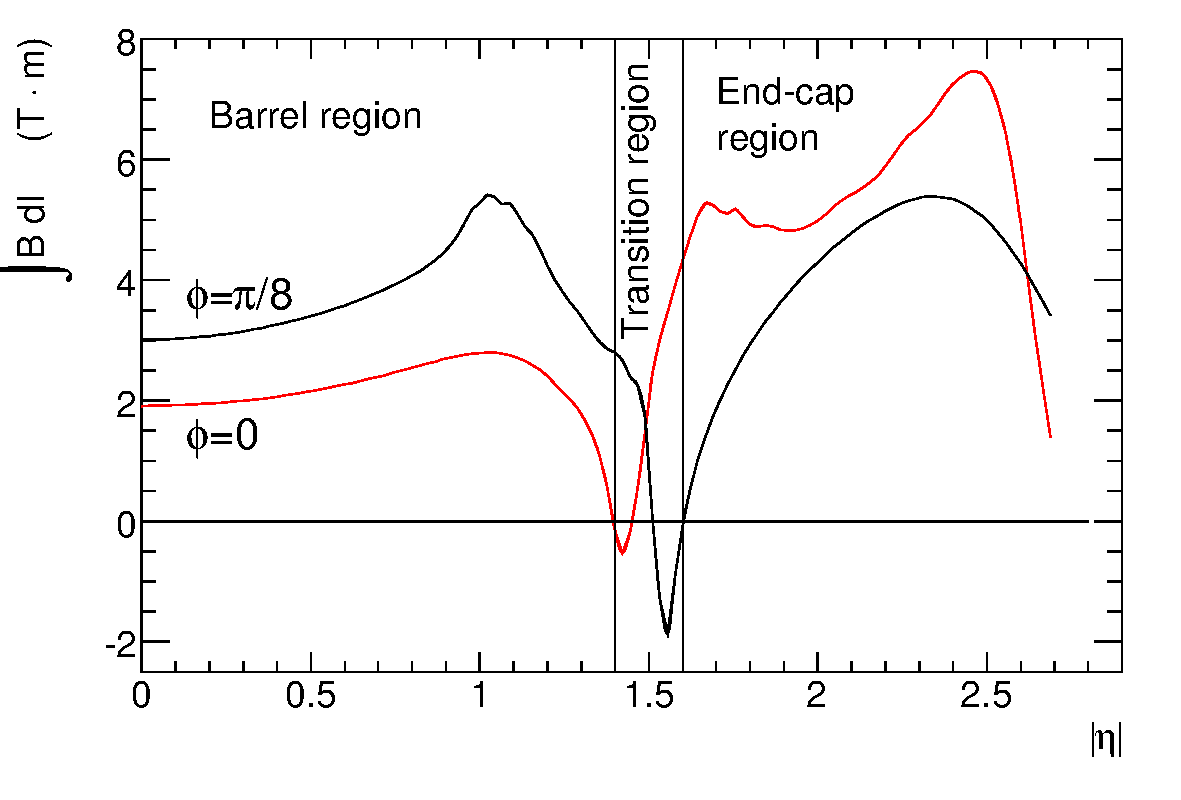
\includegraphics[width=0.6\textwidth]{figures/ATLAS_field}
    %    \caption{}
    %\end{subfigure}

   \caption{Predicted field integral as a function of $|\eta|$ for the ATLAS magnet system~\cite{ATLASPaper}}
  \label{fig:ATLAS_mag}
\end{figure}

\subsection{Trigger system}

The ATLAS trigger system searches for signatures of muons, electrons, photons, hadronically decaying $\tau$ leptons, and jets in order to save these events for further analysis. The trigger system in ATLAS is designed to reduce the maximum LHC event rate of $40\,\rm MHz$ to a more reasonable rate that can be recorded. The trigger first consists of a fast, hardware based system called the Level-$1$ (L$1$) trigger. The L$1$ trigger consists of indepdendent dedicated detector sub-components that can seed regions of interest (RoIs) for further analysis downstream. For muons, the RPCs and TGCs are used, while in the calorimeter coarsely grained sections of calorimeter cells called towers are used. Once regions of interest are seeded, a software based system called the High Level Trigger (HLT) is used to reconstruct objects and integrate information from different parts of the detector. In Run $1$ of ATLAS, the HLT consisted of two separate stages: the level $2$ (L$2$) trigger and the event filter (EF). 

The maximum trigger rate that the L$1$ trigger can handle is $75\,\rm kHz$. In the HLT, the rate of events written to disk is approximately $200\, \rm Hz$. Figure~\ref{fig:trigger_rates} shows the trigger rates for different L$1$ triggers in 2012 and 2015 for ATLAS~\cite{TriggerOps}. 

\begin{figure}[h!]
  %\vspace{20pt}
  \centering
  \captionsetup{justification=centering}

   \begin{subfigure}[t]{0.5\textwidth}
        \centering
        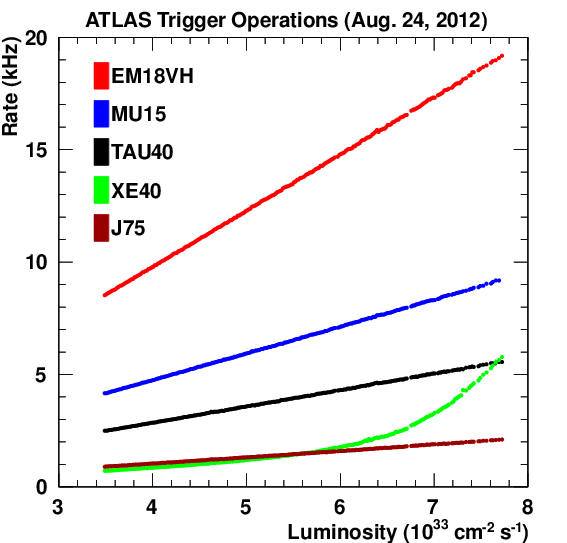
\includegraphics[width=0.7\textwidth]{figures/2012_trigger_rates}
        \caption{2012}
    \end{subfigure}%
    \begin{subfigure}[t]{0.5\textwidth}
        \centering
        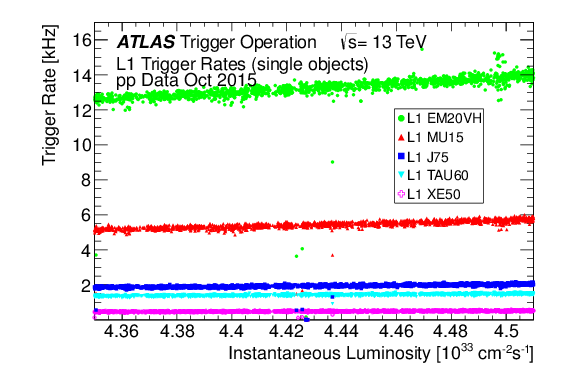
\includegraphics[width=\textwidth]{figures/2015_trigger_rate}
        \caption{2015}
    \end{subfigure}

   \caption{ATLAS trigger rates for Level-$1$ triggers as a function of instantaneous luminosity in 2012 and 2015 operation. These are single object triggers for electromagnetic clusters (EM), muons (MU), jets (J), missing energy (XE), and $\tau$ leptons (TAU). The threshold of the trigger is given in the name in $\GeV$.~\cite{TriggerOps}}
  \label{fig:trigger_rates}
\end{figure}

\subsection{ATLAS datasets}

ATLAS has collected data at center of mass energies of $7$, $8$, and $13 \TeV$. Figure~\ref{fig:lumis} shows the integrated luminosity as a function of time for each of the three collected datasets. At $\sqrt{s} = 7 \TeV$, ATLAS recorded $5.08\ifb$. Increased instantaneous luminosity in 2012 led to a larger dataset of $21.3 \ifb$ recorded at $\sqrt{s} = 8 \TeV$. After Long Shutdown $1$ (LS$1$) of the LHC and a restart in 2015, ATLAS recorded $3.9\ifb$ of data at $\sqrt{s} = 13 \TeV$. ~\cite{Lumi_Run1, Lumi_Run2} 

\begin{figure}[h!]
  %\vspace{20pt}
  \centering
  \captionsetup{justification=centering}

   \begin{subfigure}[t]{0.5\textwidth}
        \centering
        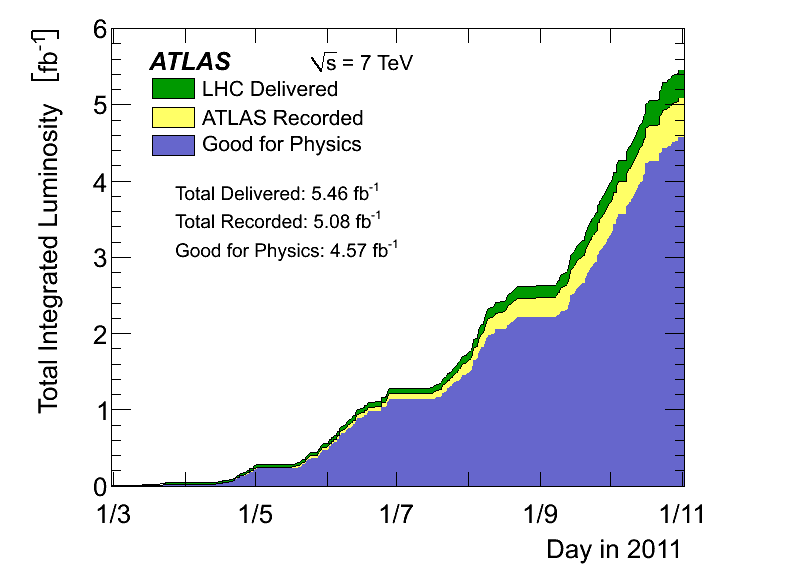
\includegraphics[width=\textwidth]{figures/ATLAS_lumi_2011}
        \caption{$\sqrt{s} = 7 \TeV$ (2011)}
    \end{subfigure}%
    \begin{subfigure}[t]{0.5\textwidth}
        \centering
        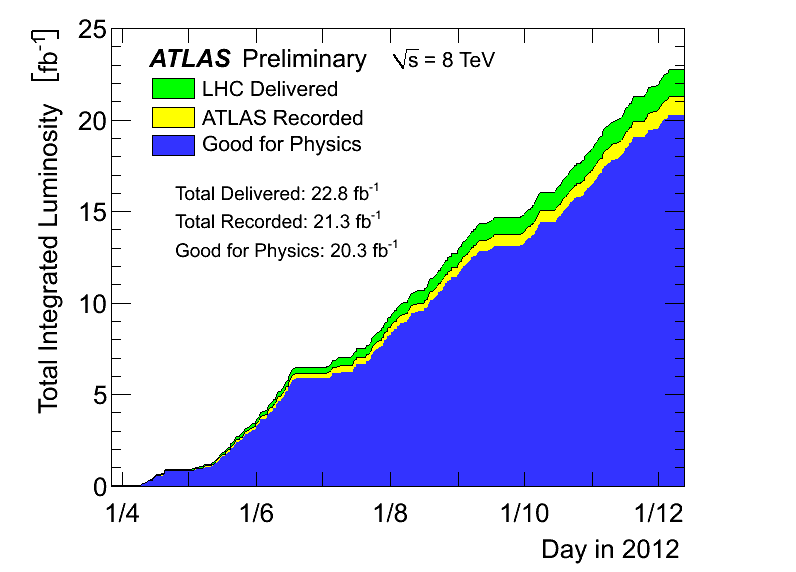
\includegraphics[width=\textwidth]{figures/ATLAS_lumi_2012}
        \caption{$\sqrt{s} = 8 \TeV$ (2012)}
    \end{subfigure}
    \begin{subfigure}[t]{0.5\textwidth}
        \centering
        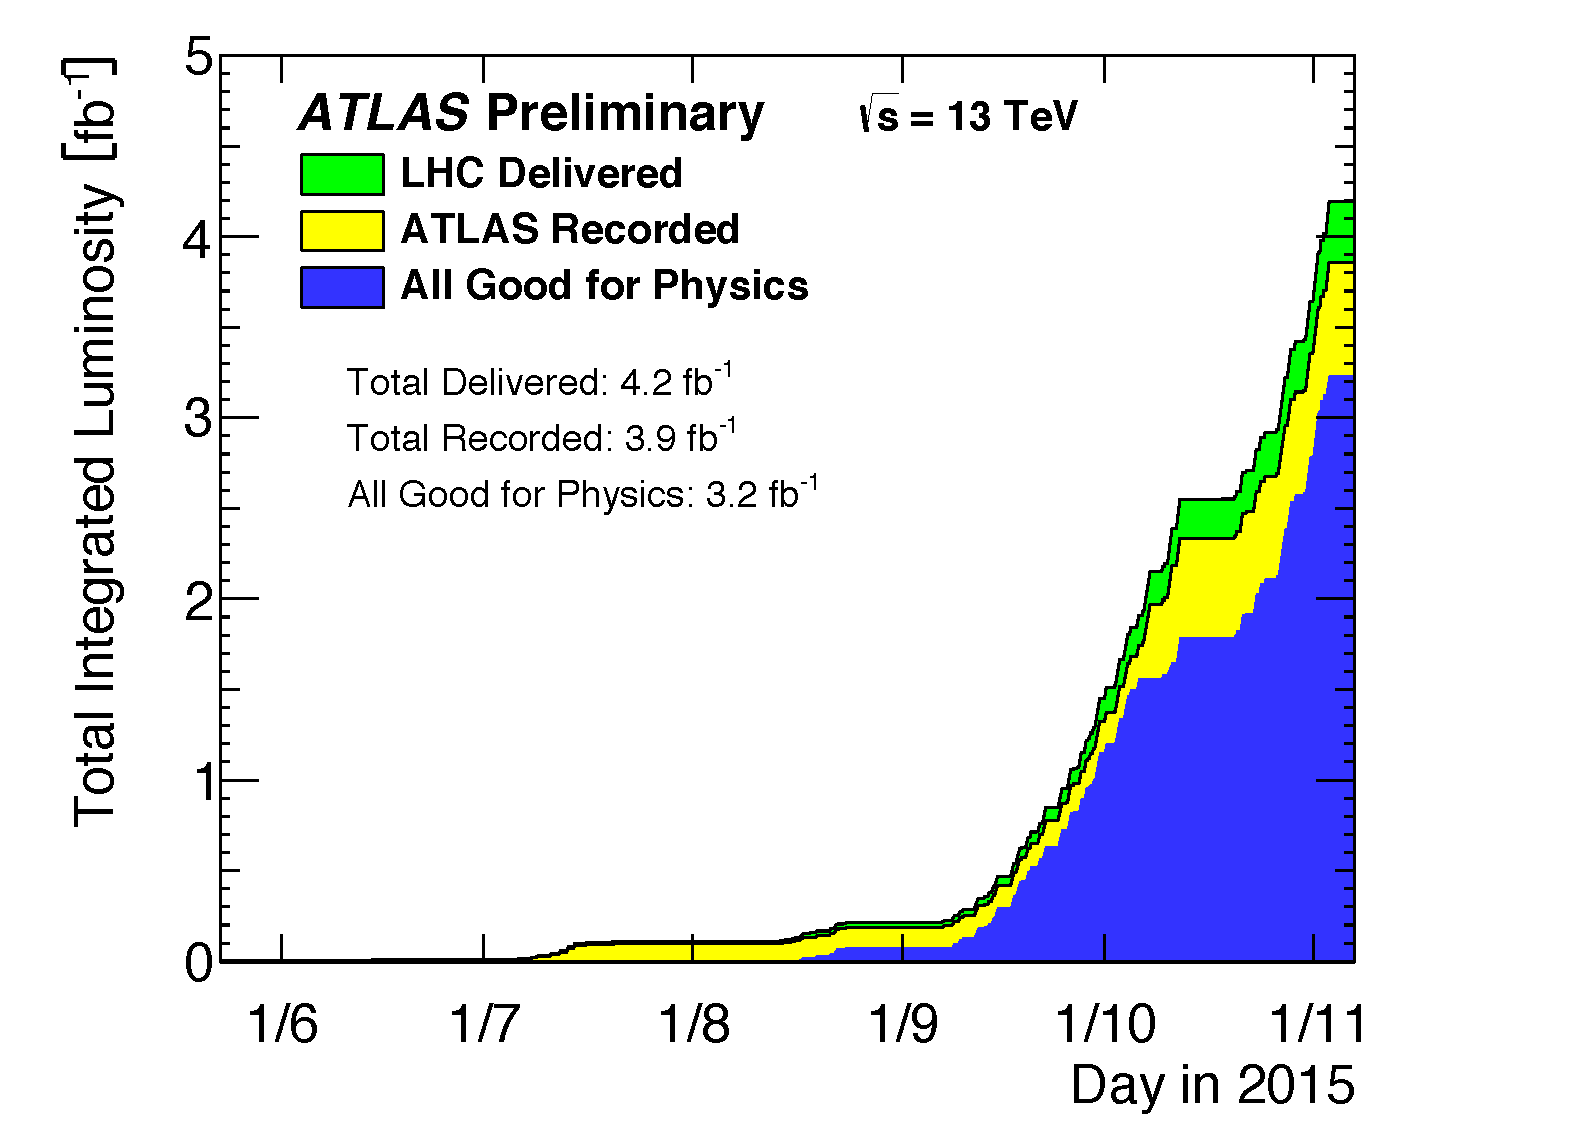
\includegraphics[width=\textwidth]{figures/ATLAS_lumi_2015}
        \caption{$\sqrt{s} = 13 \TeV$ (2015)}
    \end{subfigure}

   \caption{Instantaneous luminosity as a function of time for data recorded by ATLAS at different center of mass energies~\cite{Lumi_Run1, Lumi_Run2}}
  \label{fig:lumis}
\end{figure}


\section{The ATLAS Muon New Small Wheel Upgrade}

As the LHC continues operation, it is scheduled to be upgraded in several phases to allow it to reach higher instantaneous luminosities and thus collect larger datasets. These conditions will open new doors for study of rare physics processes but will also present interesting challenges that must be faced. ATLAS will require new detector technologies to cope with the increased background rates in the cavern in these high luminosity conditions. One such upgrade, scheduled to be installed during Long Shutdown $2$ (LS$2$) of the LHC in 2018, is the ATLAS Muon New Small Wheel (NSW) upgrade~\cite{NSW_TDR}. The NSW will replace the innermost end-cap wheel of the muon system with new technologies, as this is the part of the muon detector closest to the beam and thus suffers from the highest rates. 

\subsection{Motivation}

The motivation of the NSW is two-fold. First, the objective is to alleviate the decreased tracking efficiency that comes in a high rate environment. As figure~\ref{fig:mdt_hit_rate}, at the LHC design luminosity both the efficiency of recording hits and reconstructing track segments in the MDTs decreases at the LHC design luminosity. 

\begin{figure}[h!]
  %\vspace{20pt}
  \centering
  \captionsetup{justification=centering}

  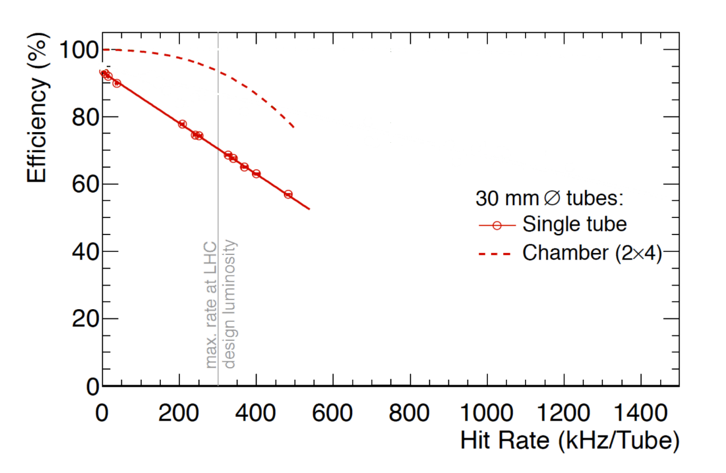
\includegraphics[width=0.7\textwidth]{figures/MDT_hit_rate}
   \caption{MDT tube hit (solid) and segment (dashed) efficiency as a function of hit rate per tube~\cite{NSW_TDR}}
  \label{fig:mdt_hit_rate}
\end{figure}

Second, the NSW will work to alleviate the rate of fake triggers arising in the endcap. Figure~\ref{fig:NSW_trig} shows the extrapolated trigger rates as a function of the $p_{T}$ threshold with and without the NSW upgrade. As the figure shows, the NSW upgrade will reduce the trigger rate by an order of magnitude compared to the current endcap trigger system. 

\begin{figure}[h!]
  %\vspace{20pt}
  \centering
  \captionsetup{justification=centering}

  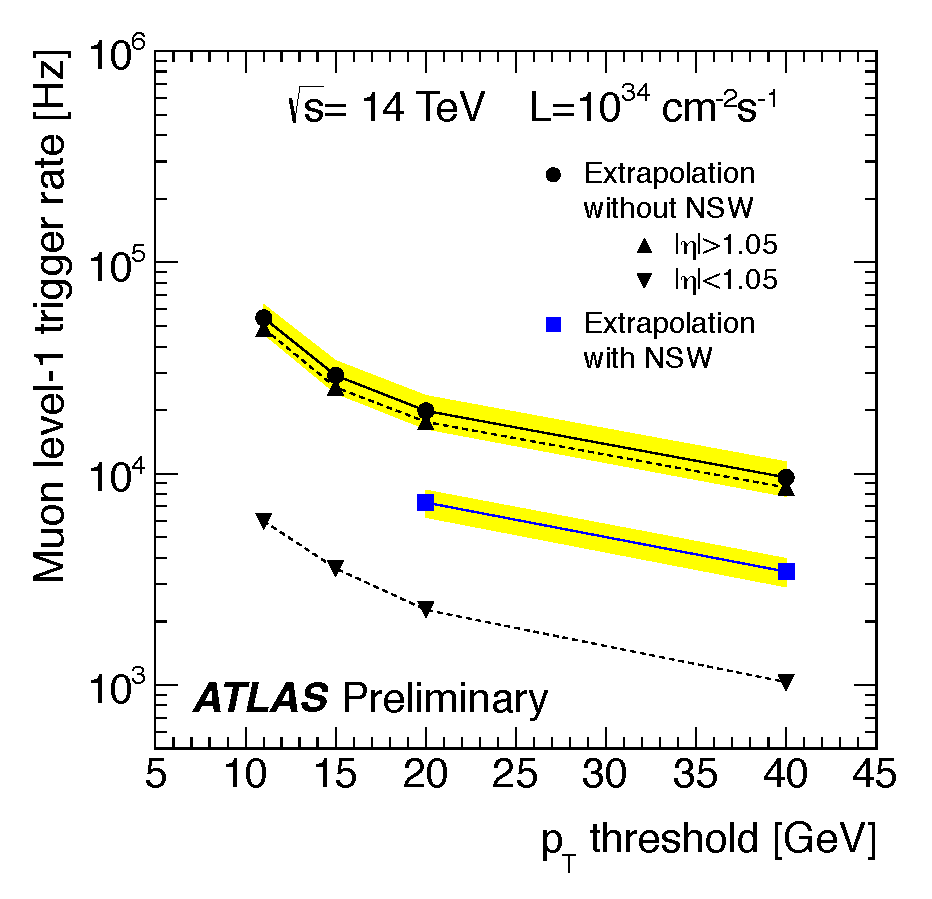
\includegraphics[width=0.6\textwidth]{figures/NSW_trigger_rate}
   \caption{Trigger rate as a function of $p_{T}$ threshold with and without the NSW upgrade~\cite{NSW_TDR}}
  \label{fig:NSW_trig}
\end{figure}

\subsection{NSW detector technologies}

The NSW will use two new detector technologies - micromesh gaseous structure detectors (micromegas) and small-strip thin gap chambers (sTGCs)~\cite{MMPaper,NSW_TDR}. Unlike the previous detectors, both of these detector technologies can be used for tracking or trigger. However, the micromegas is more suited to tracking because of its good spatial resolution, while the sTGCs have better time resolution and are more suited for the trigger. To maintain a fully redundant system, both technologies are used for both purposes. 

\subsubsection{Micromegas}

Micromegas detectors operate using a thin metallic mesh that sits approximately $100\,\mu \rm m$ away from the readout electrodes to create the amplification region. Above this mesh, there is a drift region on the order of a few mm in length capped by a drift electrode. As a charged particle traverses the detector, it ionizes gas and the electrons drift down towards readout strips. The timing of the drift can be used to reconstruct the angle of traversal of the particle. This is illustrated in figure~\ref{fig:mm}. The micromegas used in ATLAS will be resistive micromegas, where the readout electrodes are topped with resistive strips~\cite{ResistiveMM}. This alleviates the risk of sparking in the large area detectors that ATLAS will use.

In ATLAS, the micromegas drift gap will be $5\,\rm mm$ and the amplification gap will be $128\,\mu \rm m$. They are filled with the same gas mixture as the MDTs. They will be stacked in an octuplet in an XXUV-UVXX geometry, where X refers to straight strips and U and V refer to stero strips at an angle of $\pm 1.5^\circ$. This arrangement allows for measurement of the azimuthal coordinate and gives a large lever arm between the straight strips for triggering purposes. Figure~\ref{fig:mm} shows the geometry of a single micromegas detector as well as its operating principle~\cite{NSW_TDR}. 

\begin{figure}[h!]
  %\vspace{20pt}
  \centering
  \captionsetup{justification=centering}

  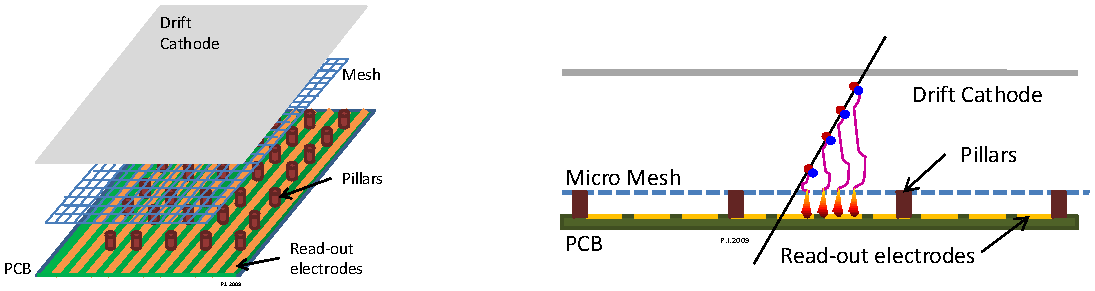
\includegraphics[width=0.85\textwidth]{figures/MM}
   \caption{Illustrations of the geometry (left) and operating principle (right) of the micromegas detector~\cite{NSW_TDR}}
  \label{fig:mm}
\end{figure}

\subsubsection{sTGCs}

The sTGCs are similar to the TGCs already described. They consist of gold-plated tungsten wires with a $1.8\,\rm mm$ pitch between two cathode planes $1.4\, \rm mm$ away from the wire plane. One cathode plane consists of strips with a $3.2\,\rm mm$ pitch (much smaller pitch than the TGCs), while the other consists of coarser pads that are used for defining regions of interest in the sTGC trigger algorithm. Figure!\ref{fig:stgc} shows the basic detector geometry. 

\begin{figure}[h!]
  %\vspace{20pt}
  \centering
  \captionsetup{justification=centering}

  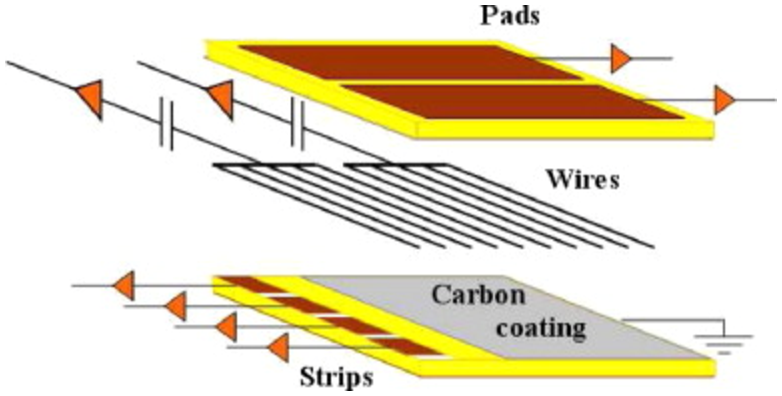
\includegraphics[width=0.5\textwidth]{figures/stgc}
   \caption{Geometry of the sTGC detector~\cite{NSW_TDR}}
  \label{fig:stgc}
\end{figure}

\subsection{Physics Impact}

Maintaining low $p_{T}$ thresholds for muons while still staying within the trigger rate budget at Level $1$ ($20\,\textrm{kHz}$) for the muon system is crucial for physics analyses to be successful in high luminosity conditions. One realm where the lepton trigger threshold is especially important is in Higgs physics. In the $\HWW$ analysis, one of the $W$ bosons is off shell and tends to decay to soft leptons. In associated production of a Higgs with a $W$, the lepton is also important because the lepton provides the main handle which allows the event to be triggered. Table~\ref{tab:NSW_trig_efficiencies} shows the impact of increasing the trigger thresholds on these analyses. It shows that either raising the threshold or using only the barrel both have significant impacts on the signal efficiency. With the NSW, the signal efficiency is largely maintained and the triggers can be unprescaled.

\begin{table}[h!]
\centering
\captionsetup{justification=centering}

%\begin{tabular*}{0.480\textwidth}{p{0.075\textwidth} p{0.180\textwidth} l}
\hspace{-10pt}
\begin{tabular}{|c|c|c|}
\hline
Threshold & $H\to b\bar{b}$ (\%) & $\HWW$ (\%) \\ \hline
$p_{T} > 20 \GeV$ & $93$ & $94$ \\ \hline
$p_{T} > 40 \GeV$ & $61$ & $75$ \\ \hline
$p_{T} > 20 \GeV$ (barrel only) & $43$ & $72$ \\ \hline
$p_{T} > 20 \GeV$ (with NSW) & $90$ & $92$ \\ \hline
\end{tabular}

\caption{
Signal efficiencies for $WH$ production with $H\to b\bar{b}$ and $H\to WW^* \to \mu \nu qq$ under different trigger configurations~\cite{NSW_TDR}.
}
\label{tab:NSW_trig_efficiencies}
\end{table}

\section{Object Reconstruction in ATLAS}

\part{Observation and measurement of Higgs boson decays to $WW*$ with
  the ATLAS detector in LHC Run 1 at $\sqrt{s} = 7$ and 8 TeV}

\begin{savequote}[75mm]
Basic research is what I am doing when I don't know what I am doing.
\qauthor{Wernher von Braun}
\end{savequote}

\chapter{$H\rightarrow WW^{*}\rightarrow \ell\nu\ell\nu$ Analysis Strategy}
\label{chap:hwwstrategy}

\section{Introduction}

This chapter presents an overview of the strategy for searching for a Higgs boson in the 
\HWWfull decay topology. Its purpose is to define in broad terms how the search and measurement are undertaken, before going into details on the specific sub-categories within the larger analysis. First, the properties of the Higgs signal are discussed and the associated backgrounds are
presented. Next, the observables used to enhance the signal to background ratio are defined. 
Finally, the parameters of interest in the search and measurement will be shown, 
along with a brief overview of the statistical treatment of the final Higgs candidates.


Following this chapter, the results of three different studies within the \HWWfull channel are shown. Chapter 4 presents a search for Higgs boson production in gluon fusion mode and the role of the $\HWW$ channel in its discovery. Chapter 5 shows the search and first observation in ATLAS of the Vector Boson Fusion (VBF) production mode of the Higgs in the $\HWW$ decay channel. Finally, chapter 6 shows the combined Run 1 $\HWW$ results for the measurement of the Higgs cross section and relative coupling strengths to other SM particles. 

\section{The \HWWfull signal in ATLAS}

\label{sec:sigtopology}

The signal studied in this and subsequent chapters is the Higgs boson in the $WW^*$ final state,
where each $W$ boson subsequently decays into a charged lepton and a neutrino. In its simplest decay path, the final state consists of two neutrinos and two charged leptons, each of which can be either an electron or a muon. If one or both of the $W$s decay to $\tau$ leptons, only leptonic decays of the $\tau$ are considered. This decay path produces additional neutrinos in the final state but still gives two charged leptons as before. Neutrinos are not detected in ATLAS, so the final state ultimately consists of two reconstructed leptons and \met (denoted as $\MET$). Final states where both of the charged leptons are electrons or muons are referred to as the ``same flavor" ($ee/\mu\mu$) final states, while those with one electron and one muon are referred to as ``different flavor" ($e\mu$ or $\mu e$).

While the basic final state consists of two leptons and $\MET$, there can be additional objects depending on the production mode of the Higgs. As described in detail in Chapter 1, if the Higgs is produced via vector boson fusion production, there will be two additional forward jets in the event. Even in gluon fusion, one or more jets can be produced through initial state radiation from the incoming gluons. Because of the varying background composition as a function of jet multiplicity, each bin in this variable has its own dedicated requirements applied in the search and measurement. The $\Njet = 0$ and $\Njet = 1$ bins are dedicated to gluon fusion production, while the $\Njet \geq 2$ bin has separate dedicated searches for ggF and VBF production. 

\begin{figure}[h!]
  %\vspace{20pt}
  \centering
  \captionsetup{justification=centering}
  %\vspace{-20pt}
  %\hspace*{-32pt}
  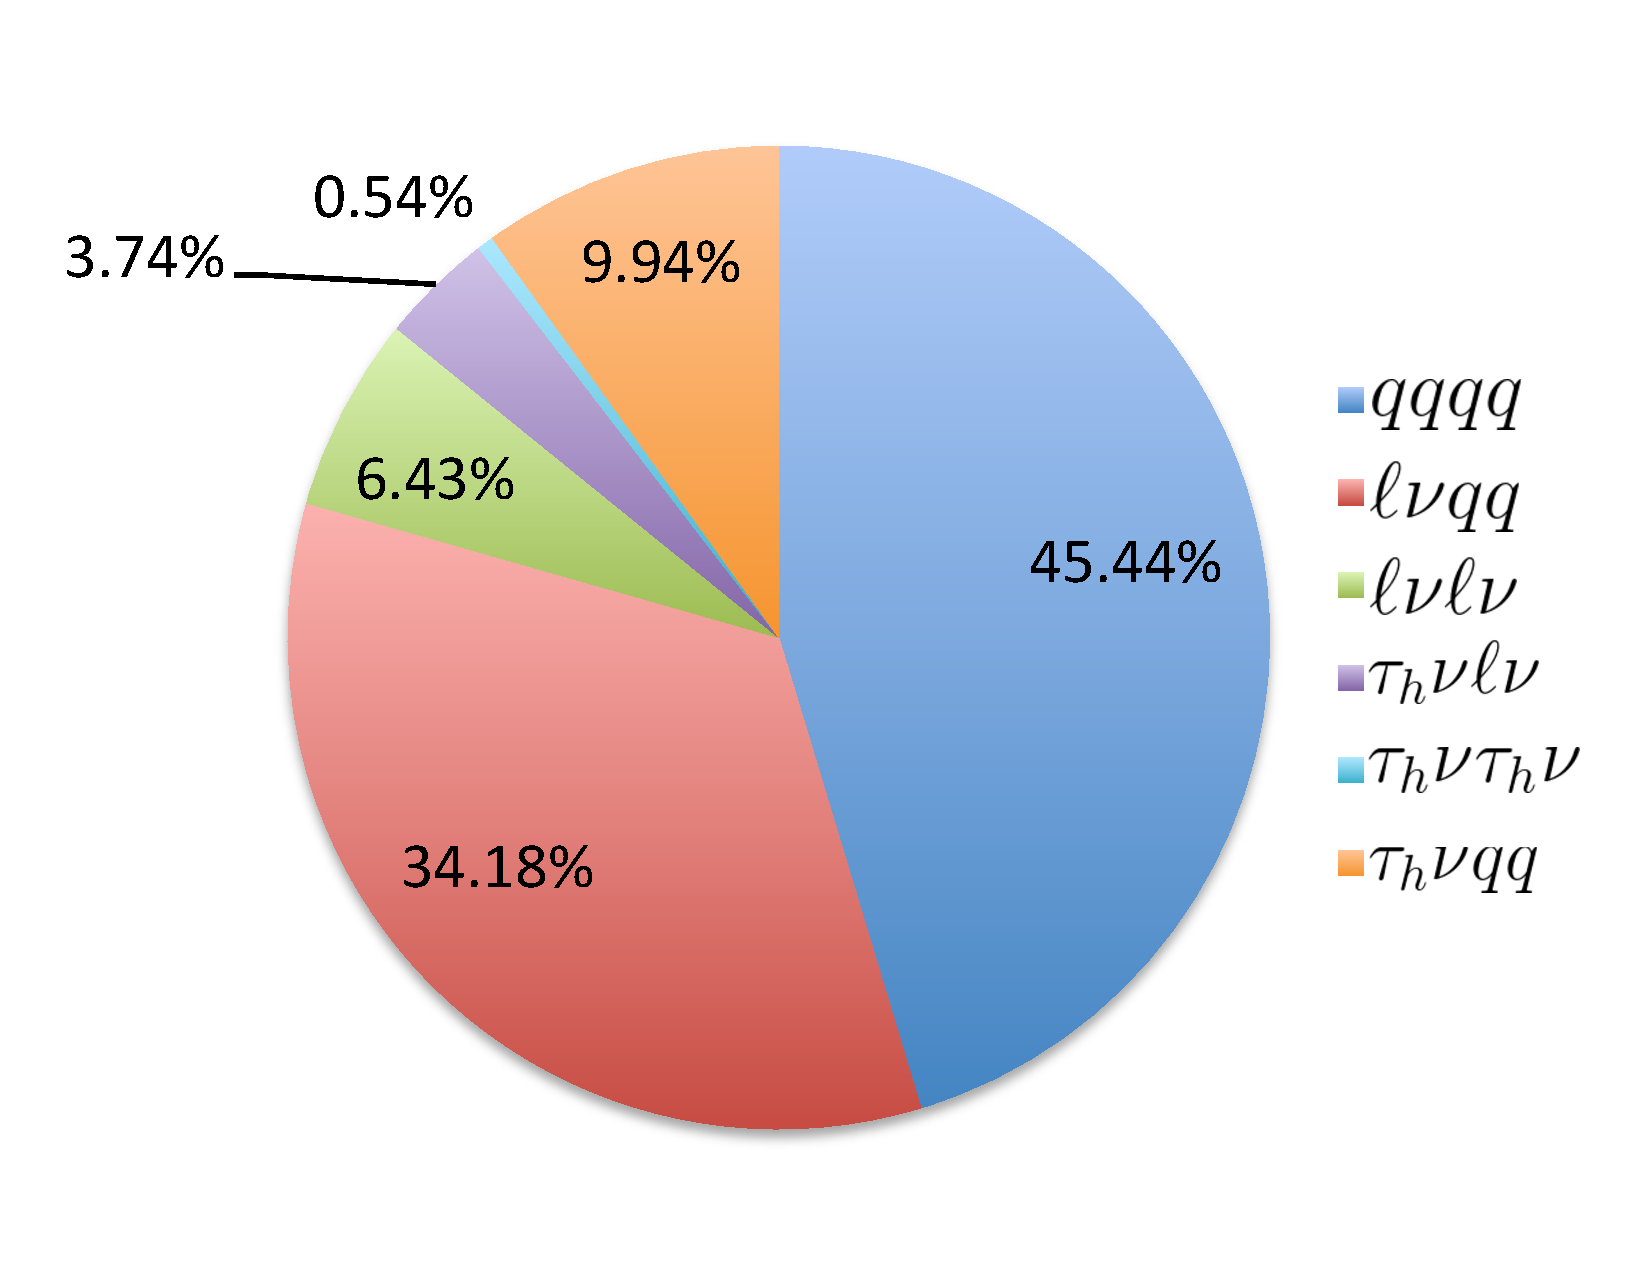
\includegraphics[width=0.7\textwidth]{figures/WWBR}
  %\vspace{-20pt}
  \caption{Branching ratios for a $WW$ system. $q$ refers to quarks. $\ell$ can be either an electron or muon, and the leptonic branching ratios of the $\tau$ are included. For example, the $\ell\nu qq$ final state includes one $W$ decaying to $e\nu$, $\mu \nu$, or $\tau \nu$. $\tau_h$ refer to hadronic decays of the $\tau$.}
  \label{fig:WWBR}
\end{figure}


Figure~\ref{fig:WWBR} shows the relative branching fractions for the $\HWW$ process, calculated from the Particle Data Group values for the $W$ and $\tau$ branching ratios\cite{pdg}. The largest branching ratio is both $W$ bosons decaying to quark pairs at 45.44\%. The next largest is one $W$ decaying leptonically and the other decaying to quarks, a branching ratio of 34.18\%. In all cases, $\ell$ denotes either an electron or muon, and the leptonic branching ratios of the $\tau$ are included. For example, the $\ell\nu qq$ final state includes one $W$ decaying to $e\nu$, $\mu \nu$, or $\tau \nu$. In the case of the $W\to\tau\nu$ decay, the $\tau$ lepton then decays to an electron or muon via $\tau \to \nu_\tau \ell \nu_\ell$. Final states with a $\tau_h$ refer to hadronic decays of the $\tau$. The branching ratio to the $\ell\nu\ell\nu$ final state is 6.43\%. 

While the $\ell\nu\ell\nu$ final state is not a large fraction of the branching ratio, there are significant advantages in this channel. First, both the $qqqq$ and $\ell\nu qq$ channels suffer from a large QCD multijet background, which is often difficult to model. Second, events in the the $\ell\nu\ell\nu$ channel in data can be triggered more efficiently due to the presence of two leptons. 

\section{Background processes}

Many processes from the Standard Model can also produce a final state with two leptons and \met. This section lists the dominant backgrounds to Higgs production. It gives general descriptions of how the backgrounds mimic Higgs production and how they can be reduced. Table\ref{tab:bkgtable} summarizes the different processes. 

\subsection{Standard Model WW production}

\begin{figure}[h!]
  %\vspace{20pt}
  \centering
  \captionsetup{justification=centering}

  %\hspace*{-32pt}
  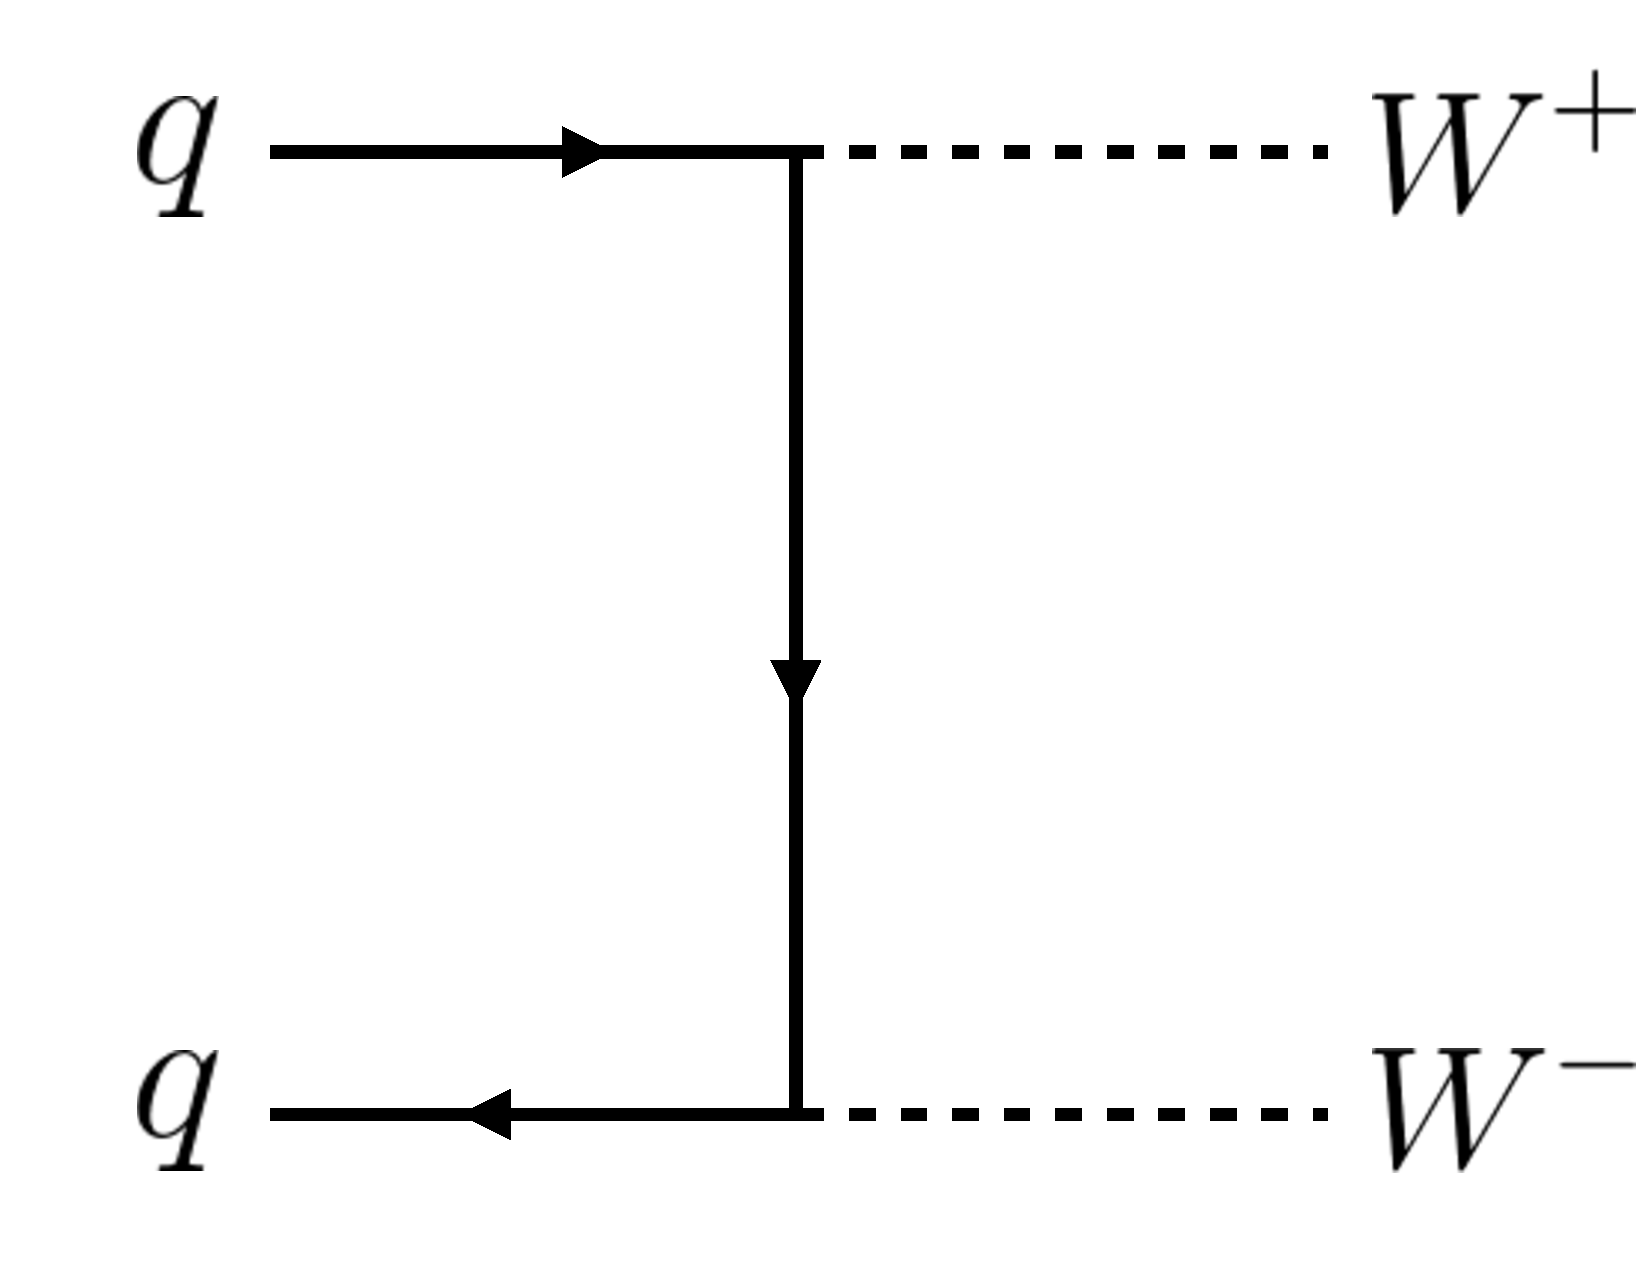
\includegraphics[width=0.4\textwidth]{figures/Feyn_SMWW}
  \caption{Feynman diagram for Standard Model WW production}
  \label{fig:SMWWdiagram}
\end{figure}

Non-resonant Standard Model diboson production, as shown in figure~\ref{fig:SMWWdiagram}, is an irreducible background to Higgs boson production in the WW final state. It produces the same exact final state objects, namely leptonically decaying W bosons. There are no additional objects in the final state that allow for background reduction. Therefore the analysis solely relies on the correlations between the leptons to reduce this background. 

\subsection{Top quark production}

Production of top quarks, either in pairs ($\ttbar$ production) or singly (e.g. $Wt$ production), can also mimic Higgs production. Because top quarks decay via $t\TO Wb$, top pair production can produce a final state with two W bosons that then decay leptonically. In this case, however, there are two additional jets from the bottom quarks in the final state. This allows the analysis to veto on the presence of jets identified as originating from a $b$ in order to reduce the size of the background. 

Single top production can occur via $s$-channel, $t$-channel, or associated production ($Wt$). The mode which most closely resembles the Higgs final state is $Wt$. In this case, there are two real $W$ bosons produced, as with $\ttbar$. However, the decay of the single top quark will still also produce one $b$-jet, meaning a $b$ veto will reduce this background as well. 

Figure~\ref{fig:Topdiagram} shows the Feynman diagrams for $\ttbar$ and $Wt$ production.  

\begin{figure}[h!]
  %\vspace{20pt}
  \centering
  \captionsetup{justification=centering}

  %\hspace*{-32pt}
  \raisebox{-0.5\height}{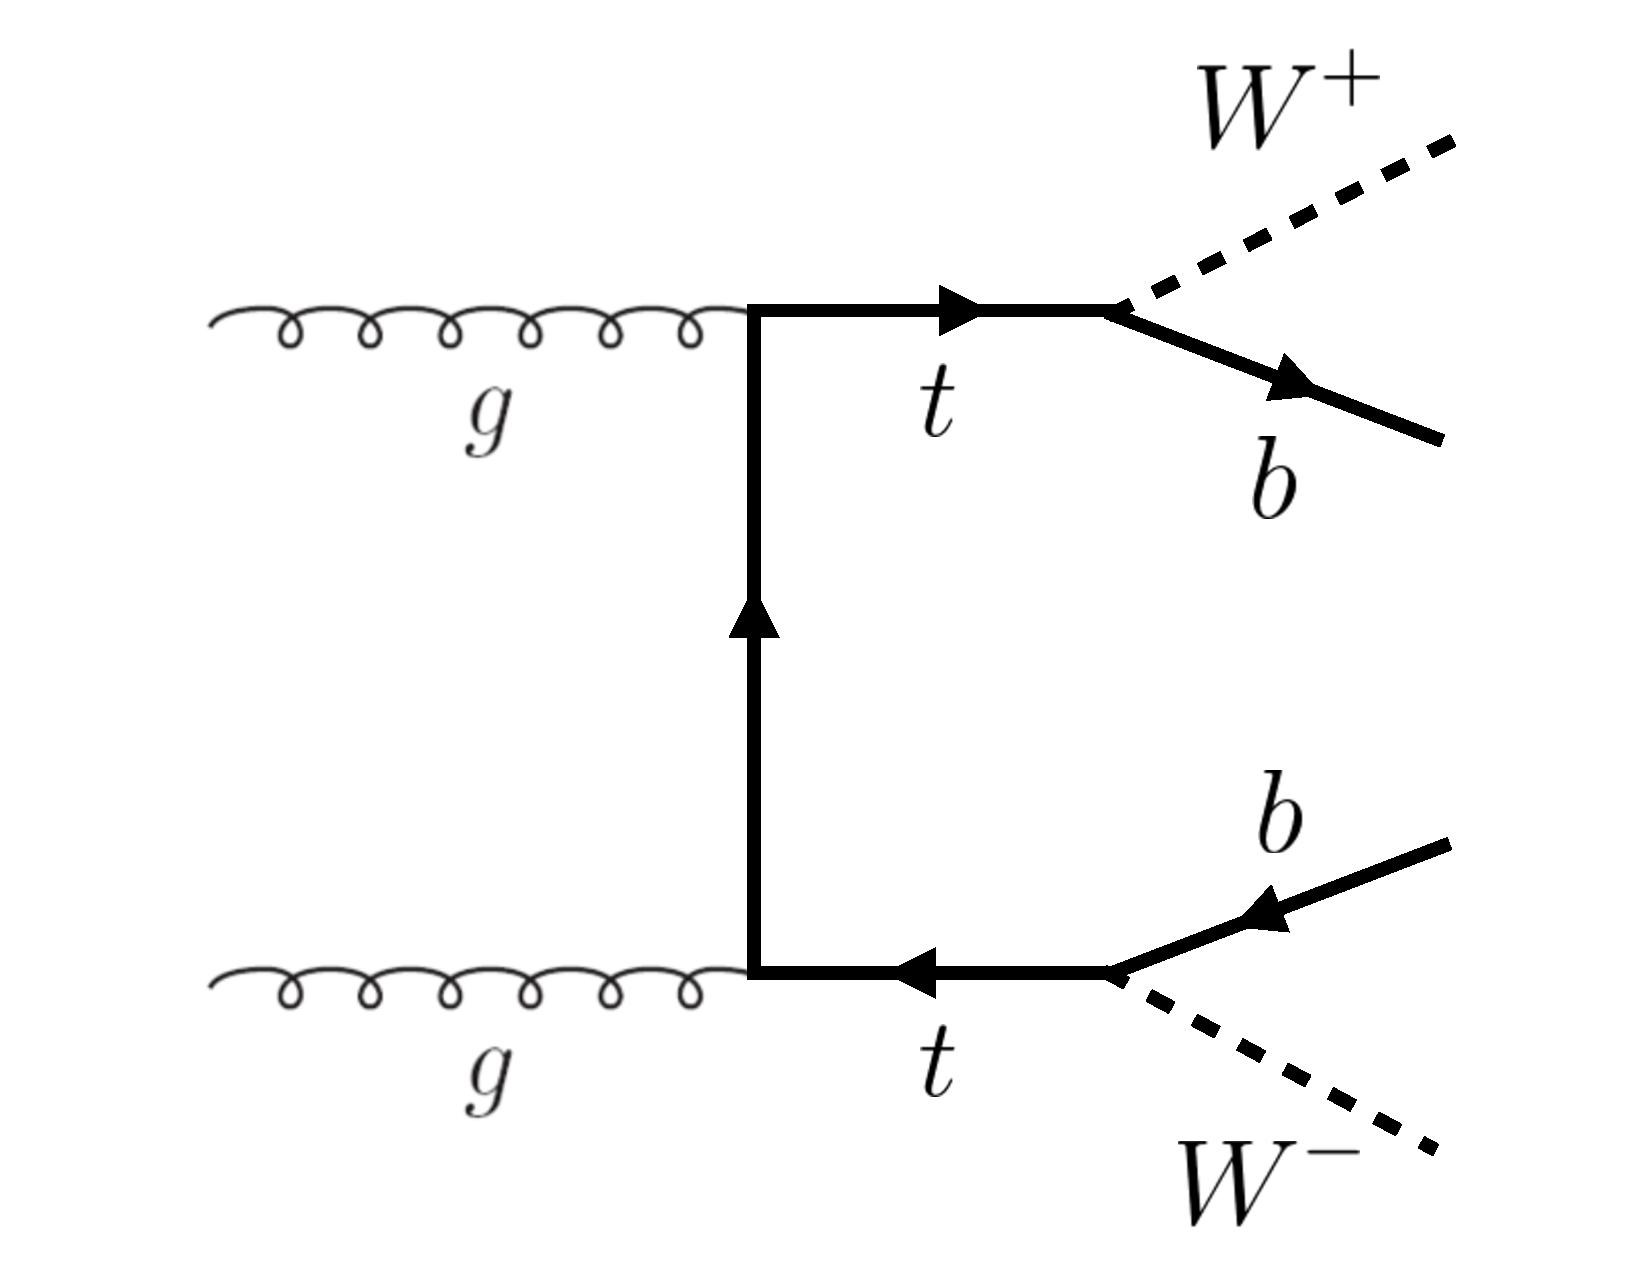
\includegraphics[width=0.4\textwidth]{figures/Feyn_ttbar}}
  \hspace{20pt}
  \raisebox{-0.5\height}{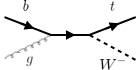
\includegraphics[width=0.4\textwidth]{figures/Feyn_Wt}}
  \caption{Feynman diagrams for top pair production (left) and $Wt$ production (right)}
  \label{fig:Topdiagram}
\end{figure}

\subsection{$W$+jets background}

Single $W$ boson production, in association with jets, is a unique background. The other background considered so far have all included real leptons in the final state. In this case, however, only one real lepton from the decay of a $W$ exists in the final state. The second reconstructed lepton can arise from two different cases. First, the lepton may truly be an algorithm ``fake", or a jet misidentified as a lepton by either the electron or muon reconstruction algorithms. Second, the lepton may be a real lepton but coming from semi-leptonic decays of particles inside the shower of the jet. This background can be reduced by requiring that the reconstructed lepton have little activity surrounding it in the calorimeter (also known as an ``isolated" lepton). Figure~\ref{fig:Wdiagram} shows the Feynman diagram for $W$+jets production. 


\begin{figure}[h!]
  %\vspace{20pt}
  \centering
  \captionsetup{justification=centering}

  %\hspace*{-32pt}
  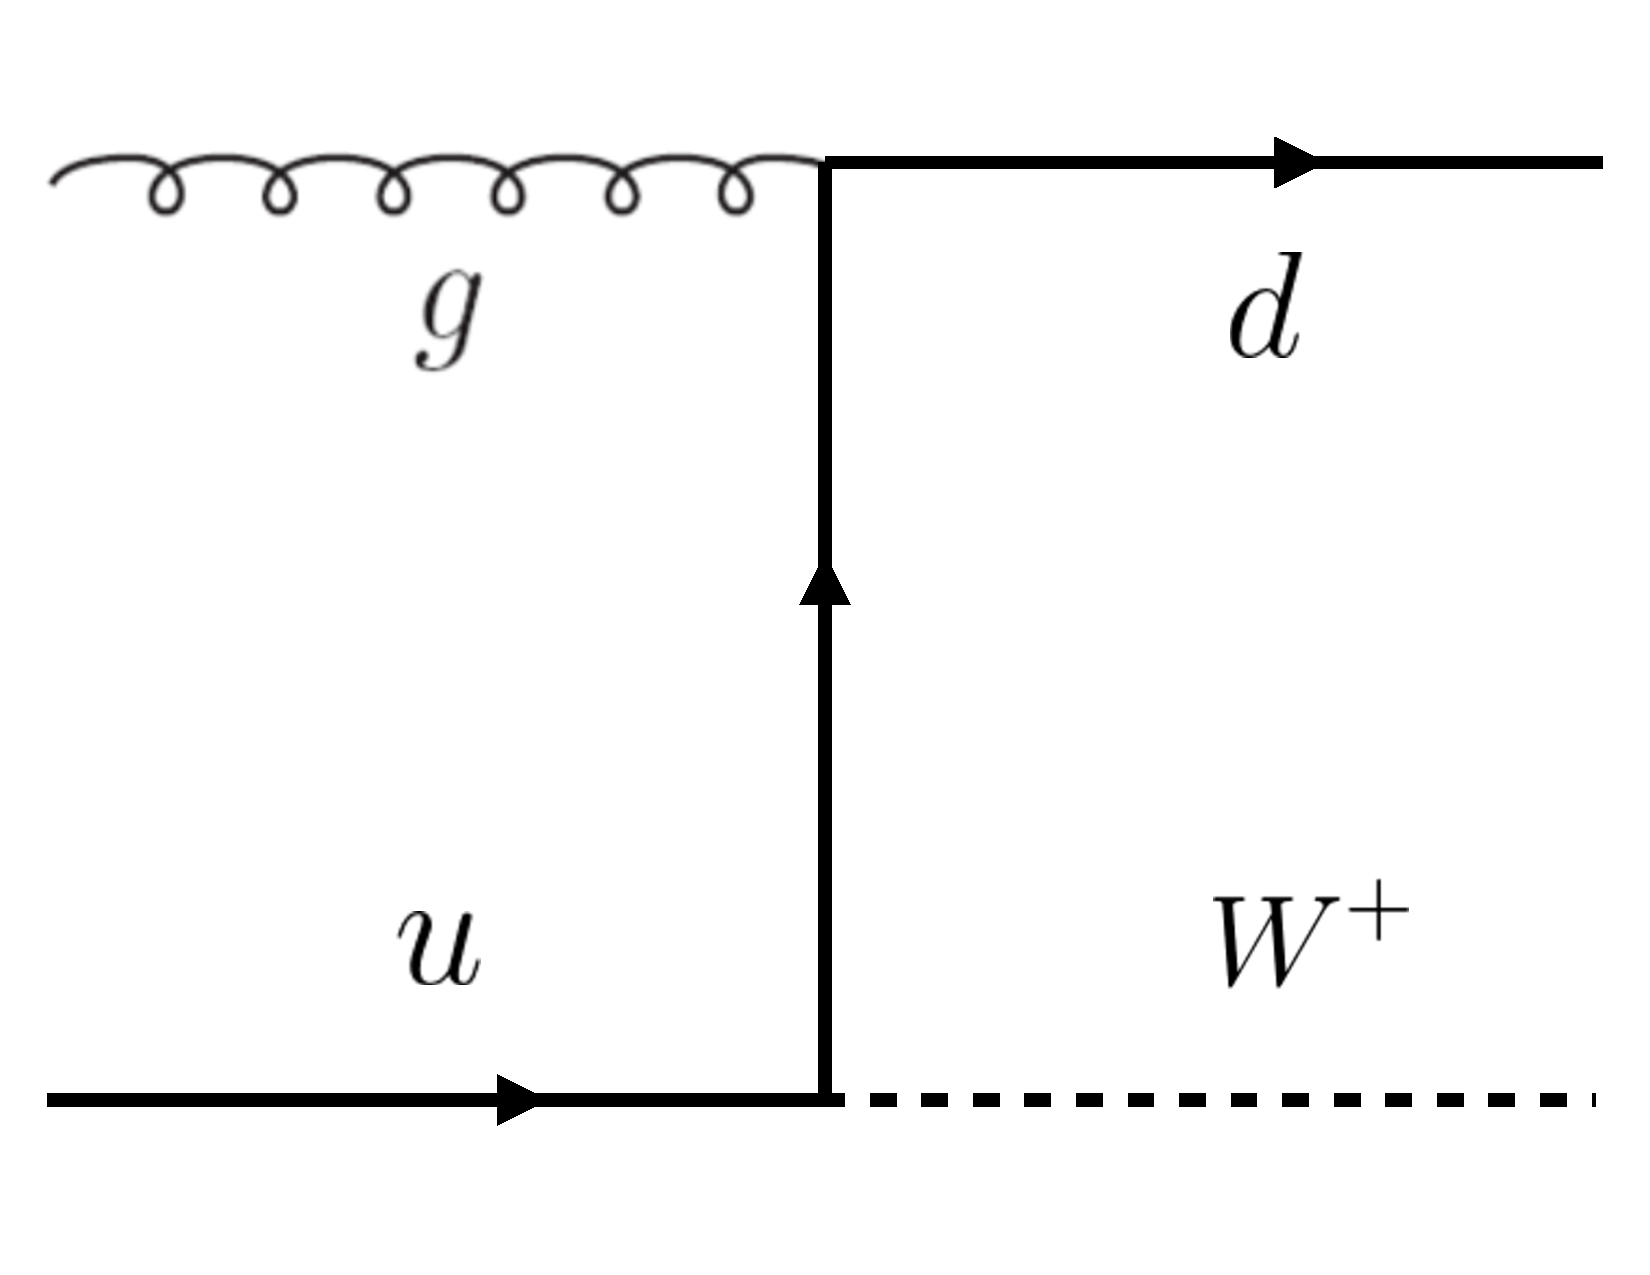
\includegraphics[width=0.4\textwidth]{figures/Feyn_W}
  \caption{An example Feynman diagram of $W$+jets production}
  \label{fig:Wdiagram}
\end{figure}

\subsection{$Z/\gamma^{*}$+jets background}

Production of a $Z/\gamma^{*}$  in association with jets (also known as Drell-Yan) is also a background to Higgs production. In particular, the same flavor final states have a large $Z$+jets background, as the $Z$ decays into two leptons of the same flavor. (This background also enters the different flavor final state through the leptonic decays of $Z\TO\tau\tau$). Figure~\ref{fig:Zdiagram} shows the production of a $Z$ in association with one jet. Because there are no neutrinos in this final state, variables like $\MET$ can be used to reduce the background. 

\begin{figure}[h!]
  %\vspace{20pt}
  \centering
  \captionsetup{justification=centering}

  %\hspace*{-32pt}
  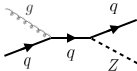
\includegraphics[width=0.4\textwidth]{figures/Feyn_Zjets}
  \caption{An example Feynman diagram of $Z$+jets production}
  \label{fig:Zdiagram}
\end{figure}

\subsection{Other (subdominant) backgrounds}

There are additional processes which contrinute to the background composition but are not produced as frequently as those listed already. The first of these are referred to as $VV$ or ``Other diboson" processes and include multiple Standard Model diboson processes, including $WZ$, $ZZ$, $W\gamma$, $W\gamma^{*}$, and $Z\gamma$ production. Additionally, there is background from QCD multijet production, where two jets are misidentified as leptons. 

\begin{table}[h!]
\centering
\captionsetup{justification=centering}

%\begin{tabular*}{0.480\textwidth}{p{0.075\textwidth} p{0.180\textwidth} l}
\hspace{-10pt}
%{\renewcommand{\arraystretch}{1.15}
\scalebox{0.9}{
\begin{tabular}{|c|c|c|}
\hline
Category & Process & Description \\ \hline
SM $WW$ & $WW\TO\ell\nu\ell\nu$ & Real leptons and neutrinos \\ \hline
\multirow{3}{*}{Top quark production} & $t\bar{t}\TO WbW\bar{b}\TO\ell\nu b \ell\nu \bar{b}$ & Real leptons, untagged $b$s \\ 
 & $tW \TO WbW \TO \ell\nu\ell\nu b $ & Real leptons, untagged $b$ \\ 
 & $t\bar{b}$, $tq\bar{b}$ & Untagged $b$, jet misidentified as lepton \\ \hline

 \multirow{2}{*}{Drell-Yan} & $\ZDY\TO ee, \mu\mu$ & ``Fake" $\MET$ \\ 
  & $\ZDY\TO \tau\tau \TO \ell\nu\nu \ell\nu\nu $& Real leptons and neutrinos \\ \hline

  \multirow{3}{*}{Other dibosons} & $ZZ \to \ell\ell \nu\nu$ & Real leptons and neutrinos \\ 
   & $W\gamma^{*}, WZ \TO \ell\nu\ell\ell, ZZ \to \ell\ell\ell\ell$ & Unreconstructed leptons \\ 
   & $W\gamma, Z\gamma$ & $\gamma$ reconstructed as $e$, unreconstructed lepton \\ \hline

   $W$+jets & $Wj \TO \ell\nu j$ & Jet reconstructed as lepton \\ \hline
   QCD multijet & $jj$ & Jets reconstructed as leptons \\ \hline
 
 \hline
\end{tabular}
%}
}
%\end{tabular*}
\caption{
  A summary of backgrounds to the \HWWfull signal 
}
\label{tab:bkgtable}
\end{table}


%\section{Object definitions}

%Selecting objects for the analysis is the first step towards rejecting background while maintaining signal acceptance. Details of the object reconstruction algorithms are defined in Chapter 2. This section presents the selections applied for reconstructed electrons, muons, jets, and \met in the final Run 1 \HWWfull analysis in order to 


\section{Shared signal region selection requirements}

As presented in section~\ref{sec:sigtopology}, there are many different combinations of objects that can define a \HWWfull final state. The multiplicity of jets and the flavor combinations of the leptons both lead to many potential signal regions. Additionally, signal regions can be optimized separately to be sensitive to the distinct production modes of the Higgs. Gluon fusion, vector boson fusion, and associated production of a Higgs all lead to unique final state topologies. Figure~\ref{fig:analysisregions} delineates the different signal regions used in the gluon fusion and vector boson fusion $\HWW$ analyses. While there are different optimizations possible in each signal region, there are also some commonly shared selections that will be described here.

\begin{figure}[h!]
  %\vspace{20pt}
  \centering
  \captionsetup{justification=centering}

  %\hspace*{-32pt}
  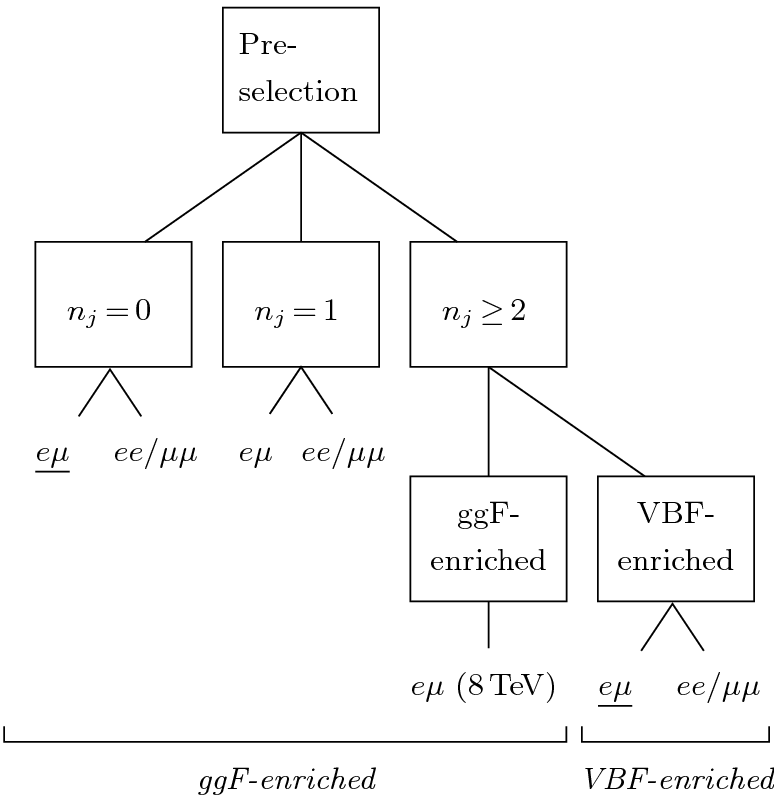
\includegraphics[width=0.6\textwidth]{figures/analysis_regions}
  \caption{An illustration of the unique analysis signal regions\cite{WW2015}}
  \label{fig:analysisregions}
\end{figure}

\subsection{Event pre-selection}

Before being sorted into the distinct signal regions, basic cuts are applied on the reconstructed objects in the event to select Higgs-like event candidates. First, two oppositely charged leptons are required. 

Once the leptons are selected, the last requirement for event pre-selection is the presence of neutrinos. As neutrinos cannot be detected directly in ATLAS, $\MET$ can be used as a proxy for the combined neutrino momentum in the transverse plane. In general, it is expected that the signal should have a harder $\MET$ spectrum than backgrounds, especially if those backgrounds did not contain neutrinos. One additional consideration when using $\MET$ is the fact that mis-measurements of objects in the detector can lead to imbalances in the transverse plane that are not due to real particles escaping the detector. One indicator that this is the case is that the $\MET$ vector in the transverse plane will be pointing in the same direction as the mis-measured object. Therefore, a new variable, $\METrel$, is used in the pre-selection. $\METrel$ is defined in equation~\ref{eqn:METrel}. 

\begin{equation}
  \begin{array}{ll}
  \multirow{2}{*}{$\METrel$ =\ \bigg\{ }
    &\!\!\!\!\MET\ \sin\dphiNear\quad\textrm{if $\dphiNear<\pi/2$}\\
    &\!\!\!\!\MET\ \phantom{\sin\dphiNear}\quad\textrm{otherwise,}
  \end{array}
\label{eqn:METrel}
\end{equation}

If the closest object to the $\MET$ vector is within $\pi/2$ radians in the transverse plane, the $\MET$ is projected away from this object. Otherwise, the normal $\MET$ vector is used. Figure~\ref{fig:METrel} shows a graphical illustration of this concept. 

\begin{figure}[h!]
  %\vspace{20pt}
  \centering
  \captionsetup{justification=centering}

  %\hspace*{-32pt}
  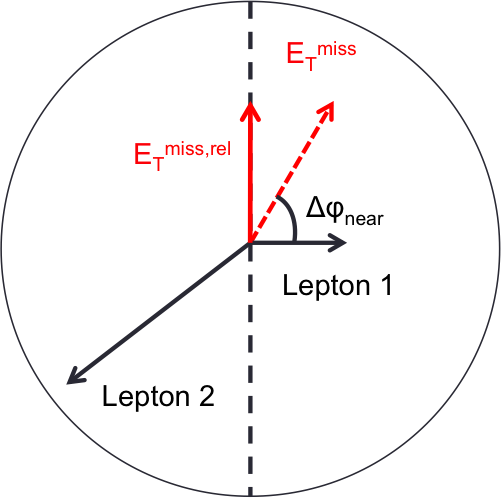
\includegraphics[width=0.6\textwidth]{figures/METrel_cartoon}
  \caption{A graphical illustration of the $\METrel$ calculation}
  \label{fig:METrel}
\end{figure}

Once both the lepton and $\MET$ pre-selections are made, the analysis can be divided into different regions according to jet multiplicity.

\subsection{Jet multiplicity}
\label{sec:jetmult}
Jet multiplicity, denoted as $\Njet$, is used to sub-divide the analysis into its distinct signal regions. The reason for this is twofold. First, different jet multiplicity bins will be more or less sensitive to different Higgs production modes. For example, the $\Njet \geq 2$ region is more sensitive to VBF production because of the two high momentum jets produced at matrix element level. For gluon fusion production to enter this bin, two initial state radiation jets must be emitted. Second, background composition varies greatly in different bins of $\Njet$. Figure~\ref{fig:njet} shows the jet multiplicity in both the different flavor and same flavor regions. It also shows the background composition in the bins of $\Nbjet$. There are a few clear trends from this distribution. The first is that the Drell-Yan background dominates in the same flavor channels for $\Njet \leq 1$. Second, the top background becomes a clear contributor to the total background for $\Njet \geq 1$. Lastly, the SM WW production dominates in the $\Njet = 0$ bin, as it is an irreducible background to $\HWW$ production. Because of these distinct features, each jet multiplicity bin is treated separately.

\begin{figure}[h!]
  %\vspace{20pt}
  \centering
  \captionsetup{justification=centering}

  %\hspace*{-32pt}
  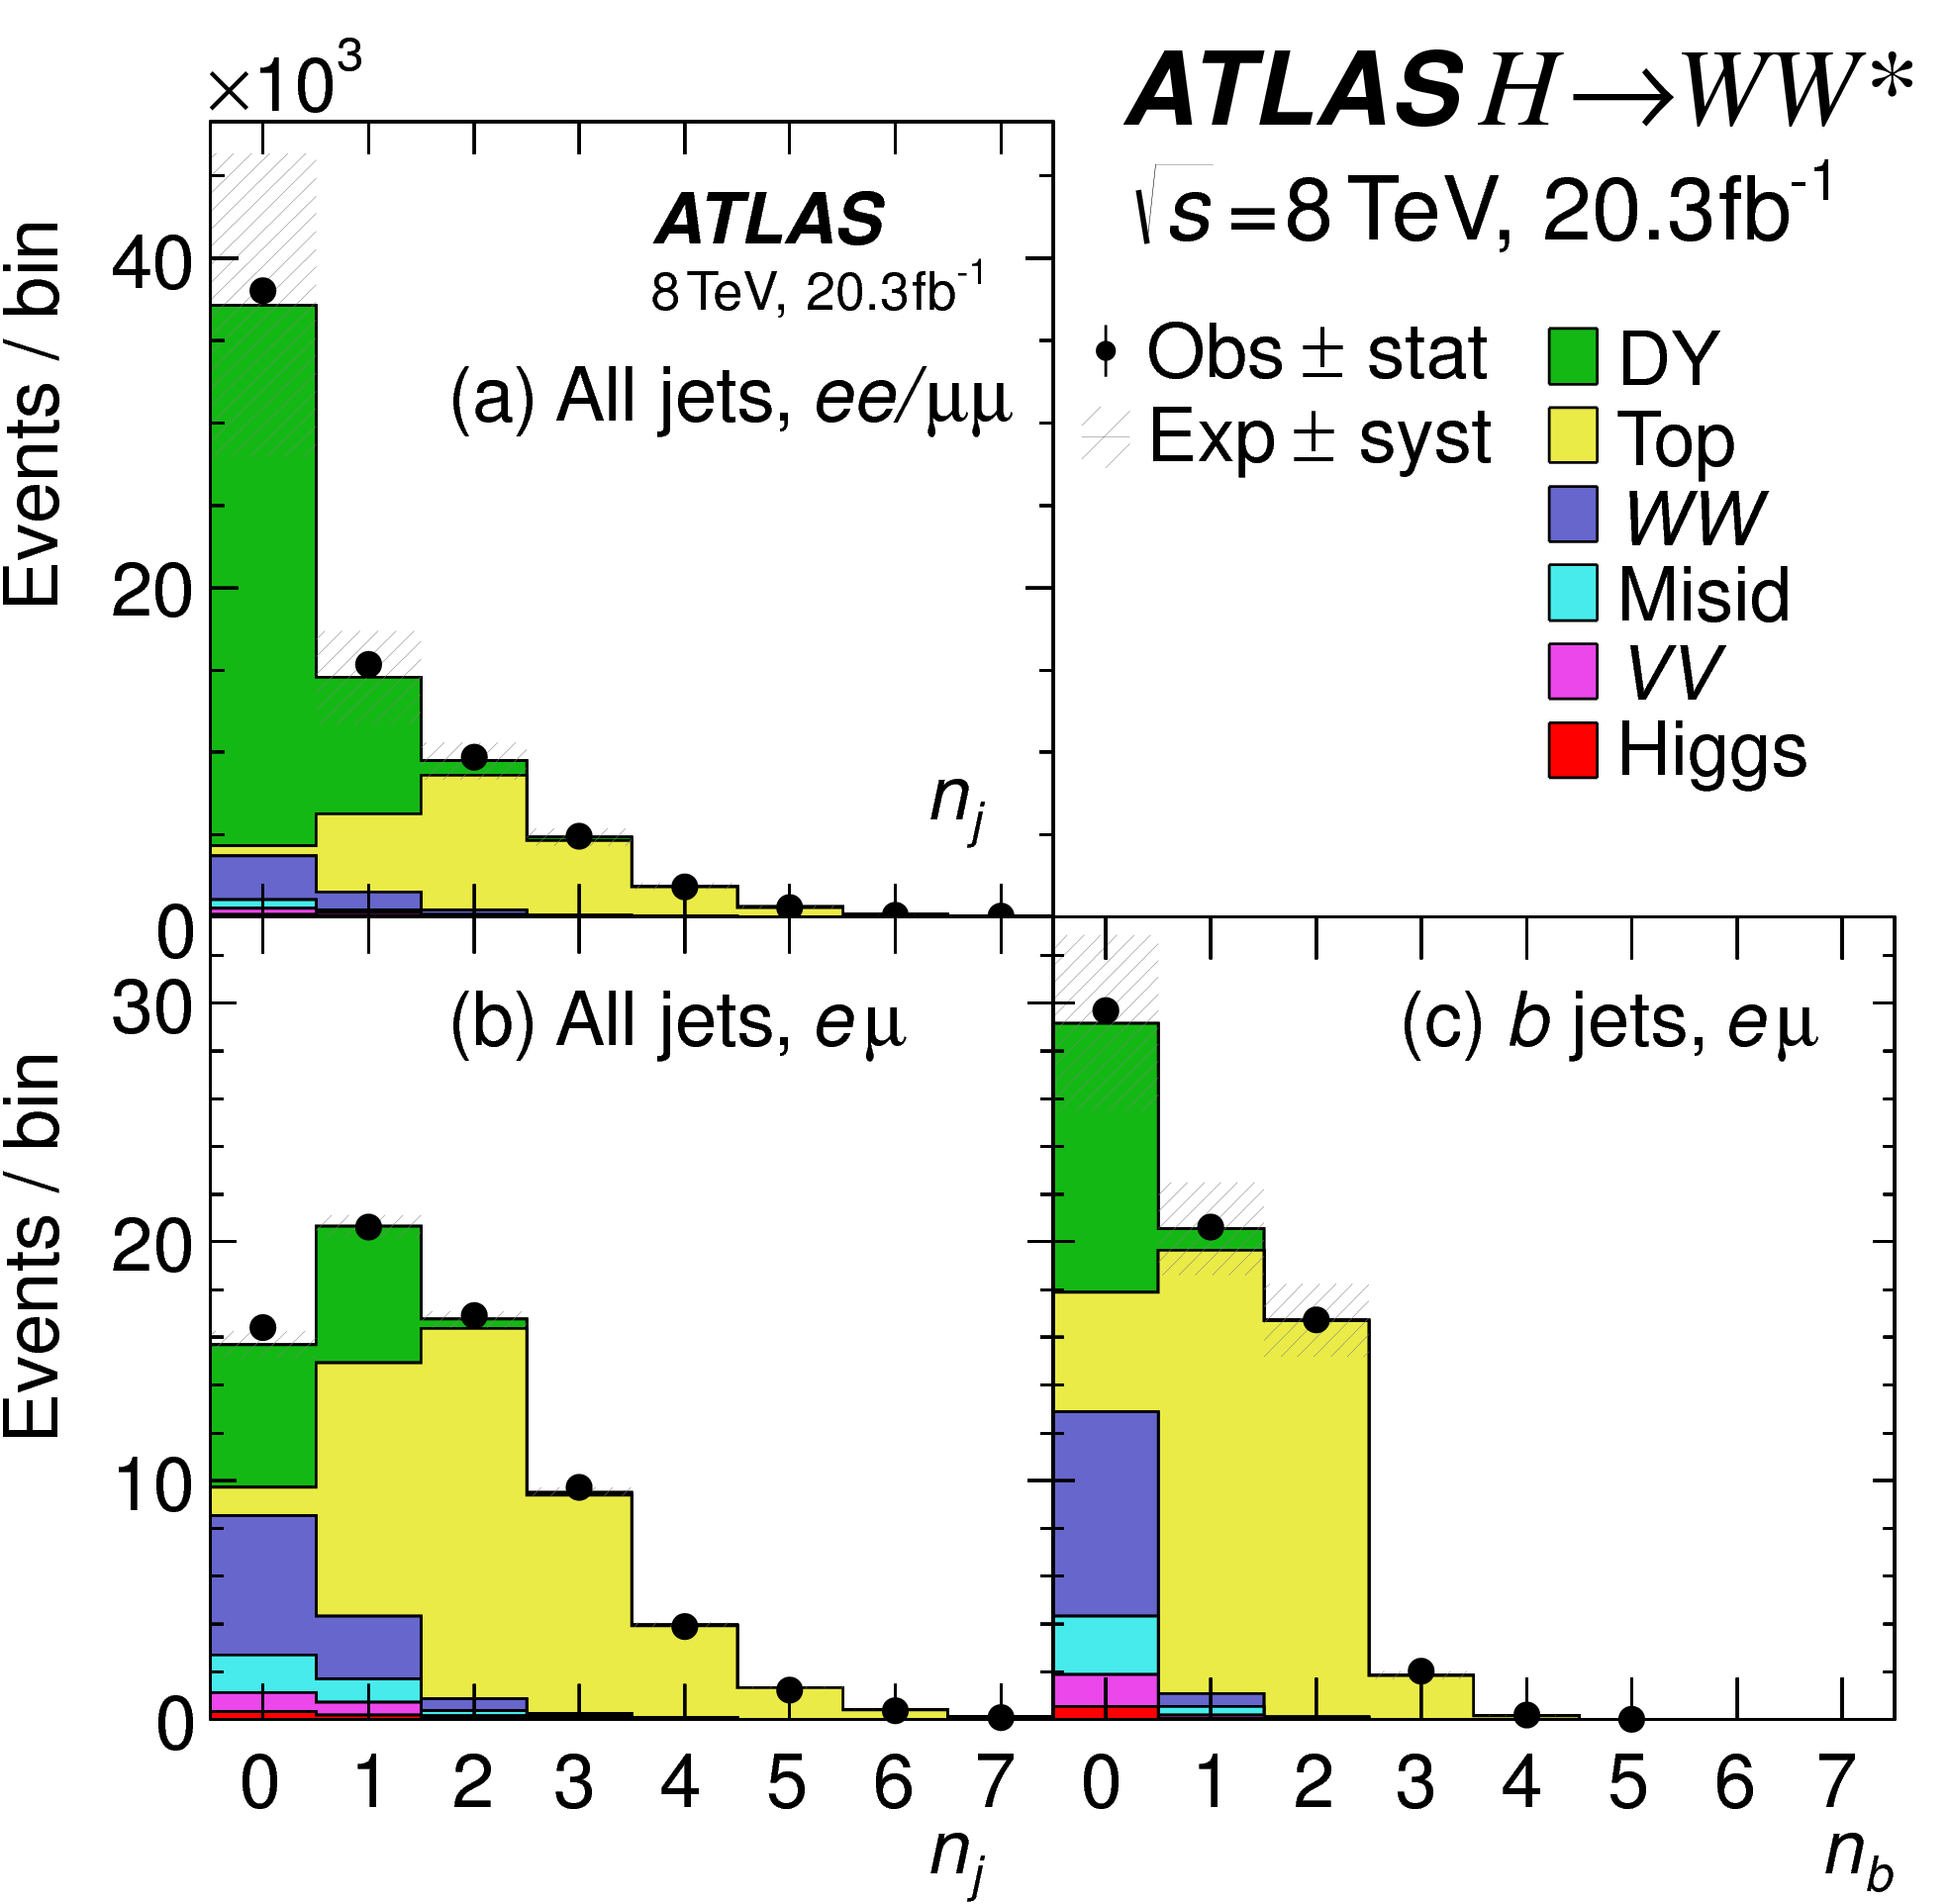
\includegraphics[width=0.6\textwidth]{figures/njet}
  \caption{Predicted backgrounds (compared with data) as a function of $\Njet$ (a and b) and $\Nbjet$ (c)}
  \label{fig:njet}
\end{figure}

\section{Background reduction in same-flavor final states}

As described in section~\ref{sec:jetmult}, the background composition of the same flavor final states is unique to that of the different flavor states. In particular, Drell Yan processes play a much larger role because the $Z/\gamma^{*}$ decays to same flavor leptons. Because real neutrinos are absent in the $\ZDY$ decays to $ee$ and $\mu\mu$, a cut on $\MET$ should largely reduce the background. However, as this section will demonstrate, with increasing pileup conditions the resolution of the calorimeter-based $\MET$ degrades greatly. Therefore, two new variables for $\ZDY$ background reduction are constructed and described in this section.

\subsection{Pileup and $\MET$ resolution}

Secondary interactions of protons in the colliding bunches of the LHC (known as pileup interactions, described in detail in Chapter 2) deposit energy into the ATLAS calorimeter on top of the energy that comes from the hard scatter process that is being searched for or analyzed. The calculation of $\MET$ is fundamentally Poissonian, as summing up all of the energy deposits in individual calorimeter cells or clusters is similar to a counting experiment. Thus, the energy resolution scales as $\sqrt{E}$, just as the error on a mean of $N$ in a Poisson distribution is $\sqrt{N}$. As more energy is deposited in the calorimter, the $\MET$ resolution degrades, meaning that the $\MET$ resolution is particularly sensitive to LHC instantaneous luminosity conditions. 

Figure~\ref{fig:Zjetseventdisplay} shows an event display of a $\ZDY$ + jets event candidate with the twenty-five reconstructed primary vertices. This display illustrates that while the interaction of interest only has tracks coming from the hardest primary vertex, all of the secondary interactions will deposit energy in the calorimeter as well.

\begin{figure}[h!]
  %\vspace{20pt}
  \centering
  \captionsetup{justification=centering}

  %\hspace*{-32pt}
  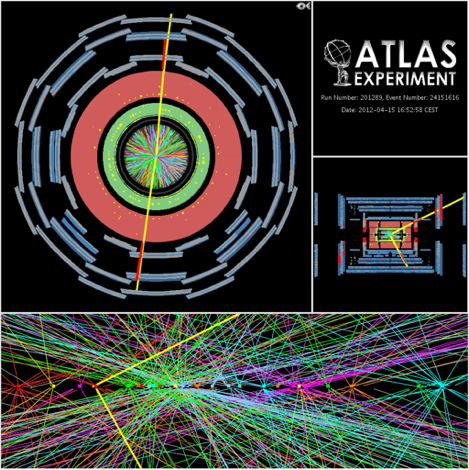
\includegraphics[width=0.6\textwidth]{figures/Zjets_EventDisplay}
  \caption{An event display of a $\ZDY$ + jets event illustrating the effect of pileup interactions}
  \label{fig:Zjetseventdisplay}
\end{figure}

Figure~\ref{fig:METResolution} shows the RMS of the $\MET$ distribution in $Z\TO\mu\mu$ events (where there are no real neutrinos) as a function of the number of the average number of interactions. Under 2011 LHC conditions, this RMS was approximately 9 \GeV, while under 2012 running conditions the resolution worsened to 12 \GeV. This worsening dilutes the efficacy of a cut on $\MET$ to reduce the $\ZDY$ background. 

\begin{figure}[h!]
  %\vspace{20pt}
  \centering
  \captionsetup{justification=centering}

  %\hspace*{-32pt}
  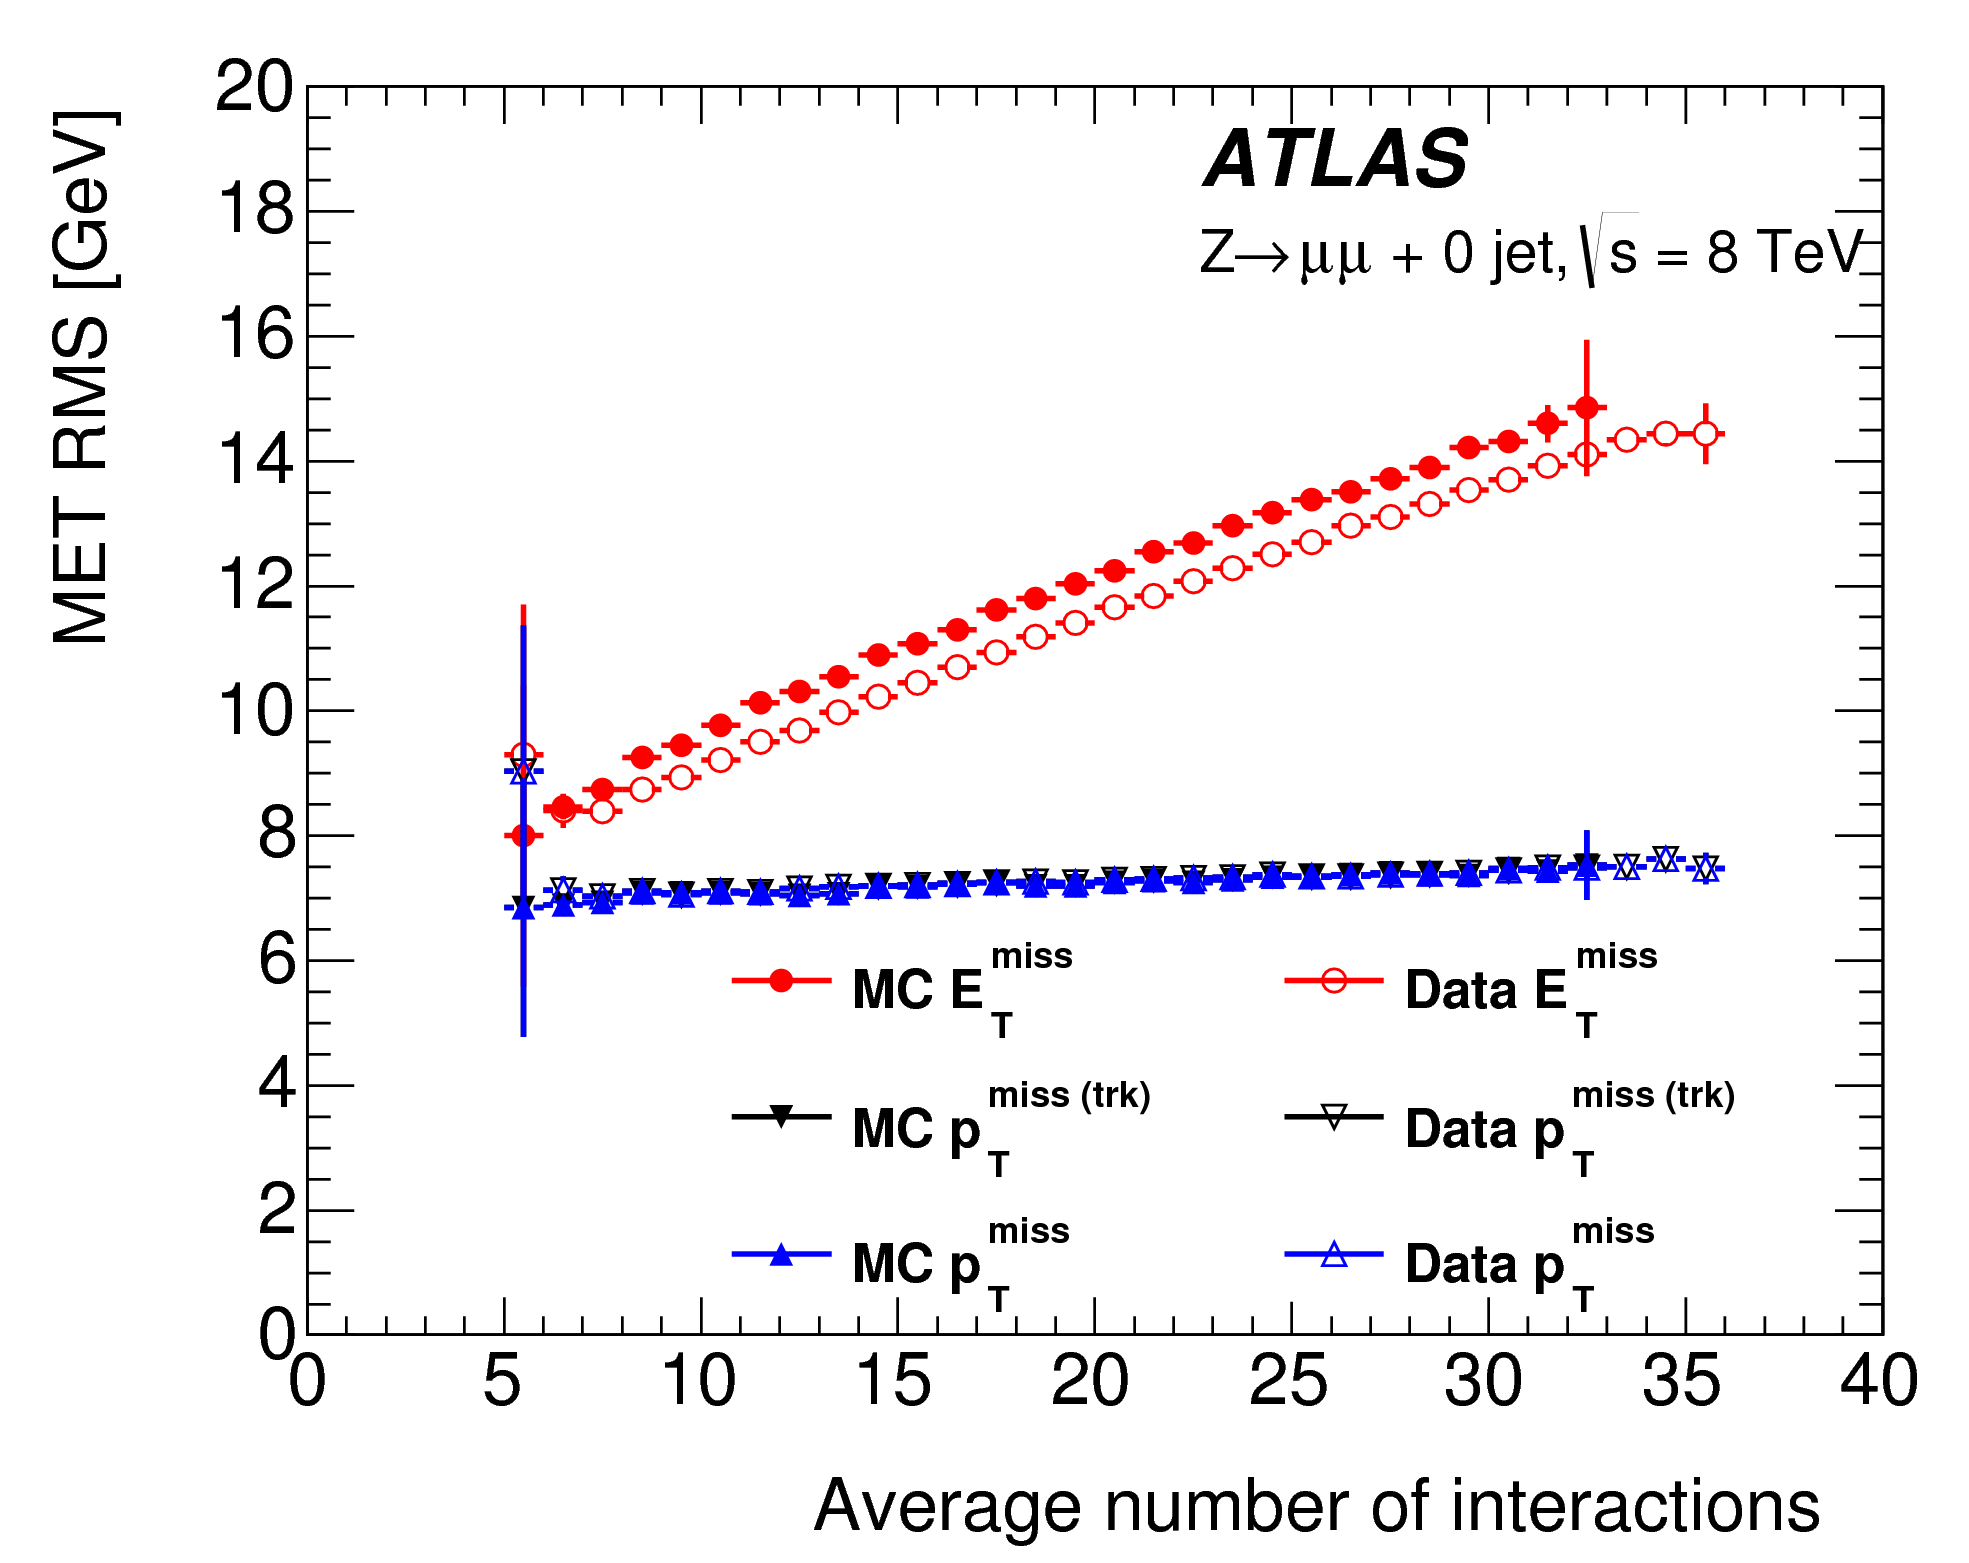
\includegraphics[width=0.6\textwidth]{figures/METResolution}
  \caption{The RMS of different missing transverse momentum definitions as a function of the average number of interactions per bunch crossing}
  \label{fig:METResolution}
\end{figure}

\subsection{Track-based definitions of missing transverse momentum}

Because the increasing number of secondary proton-proton interactions degrades calorimeter-based $\MET$ resolution, a new variable using only contributions from the primary interaction vertex is necessary to further reduce the $\ZDY$ background. While it is not possible to associate calorimeter energy deposits with a particular vertex, individual charged particle tracks in the Inner Detector are associated to unique vertices. Thus, two track-based definitions of \met, using only tracks coming from the primary vertex in the event, are used in the analysis. The simplest variable, $\MPT$, is the vectorial sum of the $\pt$ of all of the tracks from the primary vertex and the selected leptons (excluding the tracks associated with the selected leptons to avoid double counting). This is defined in equation~\ref{eqn:MPT}.

\begin{equation}
\vMPT = -\raisebox{-3.0pt}{\bigg(}%
     \displaystyle
     \sum_{\substack{\rm selected \\ \rm leptons}}\,\vpT
   + \sum_{\substack{\rm other \\ \rm tracks}}\,\vpT
   \raisebox{-3.0pt}{\bigg)},
\label{eqn:MPT}
\end{equation} 

In events with hard jets, a better resolution on the \met is obtained by including the calorimeter based measurement of the hard jets rather than the track based measurements. Thus, another variable, $\MPTj$, is defined, using the nominal measurements of $\pT$ for the selected leptons and jets and using tracks rather than calorimeter clusters for the soft component of the \met. This is defined in equation~\ref{eqn:MPTj}.

\begin{equation}
\vMPTj = -\raisebox{-3.0pt}{\bigg(}%
     \displaystyle
     \sum_{\substack{\rm selected \\ \rm leptons}}\,\vpT
   + \sum_{\substack{\rm selected \\ \rm jets}}\,\vpT
   + \sum_{\substack{\rm other \\ \rm tracks}}\,\vpT
   \raisebox{-3.0pt}{\bigg)},
\label{eqn:MPTj}
\end{equation} 

Figure~\ref{fig:METResolution} illustrates that these two new variables accomplish their intended purpose. The resolution as a function of mean number of interactions for both $\MPT$ and $\MPTj$ is much flatter compared to the dependence for $\MET$. 

\begin{figure}[h!]
  %\vspace{20pt}
  \centering
  \captionsetup{justification=centering}

  %\hspace*{-32pt}
  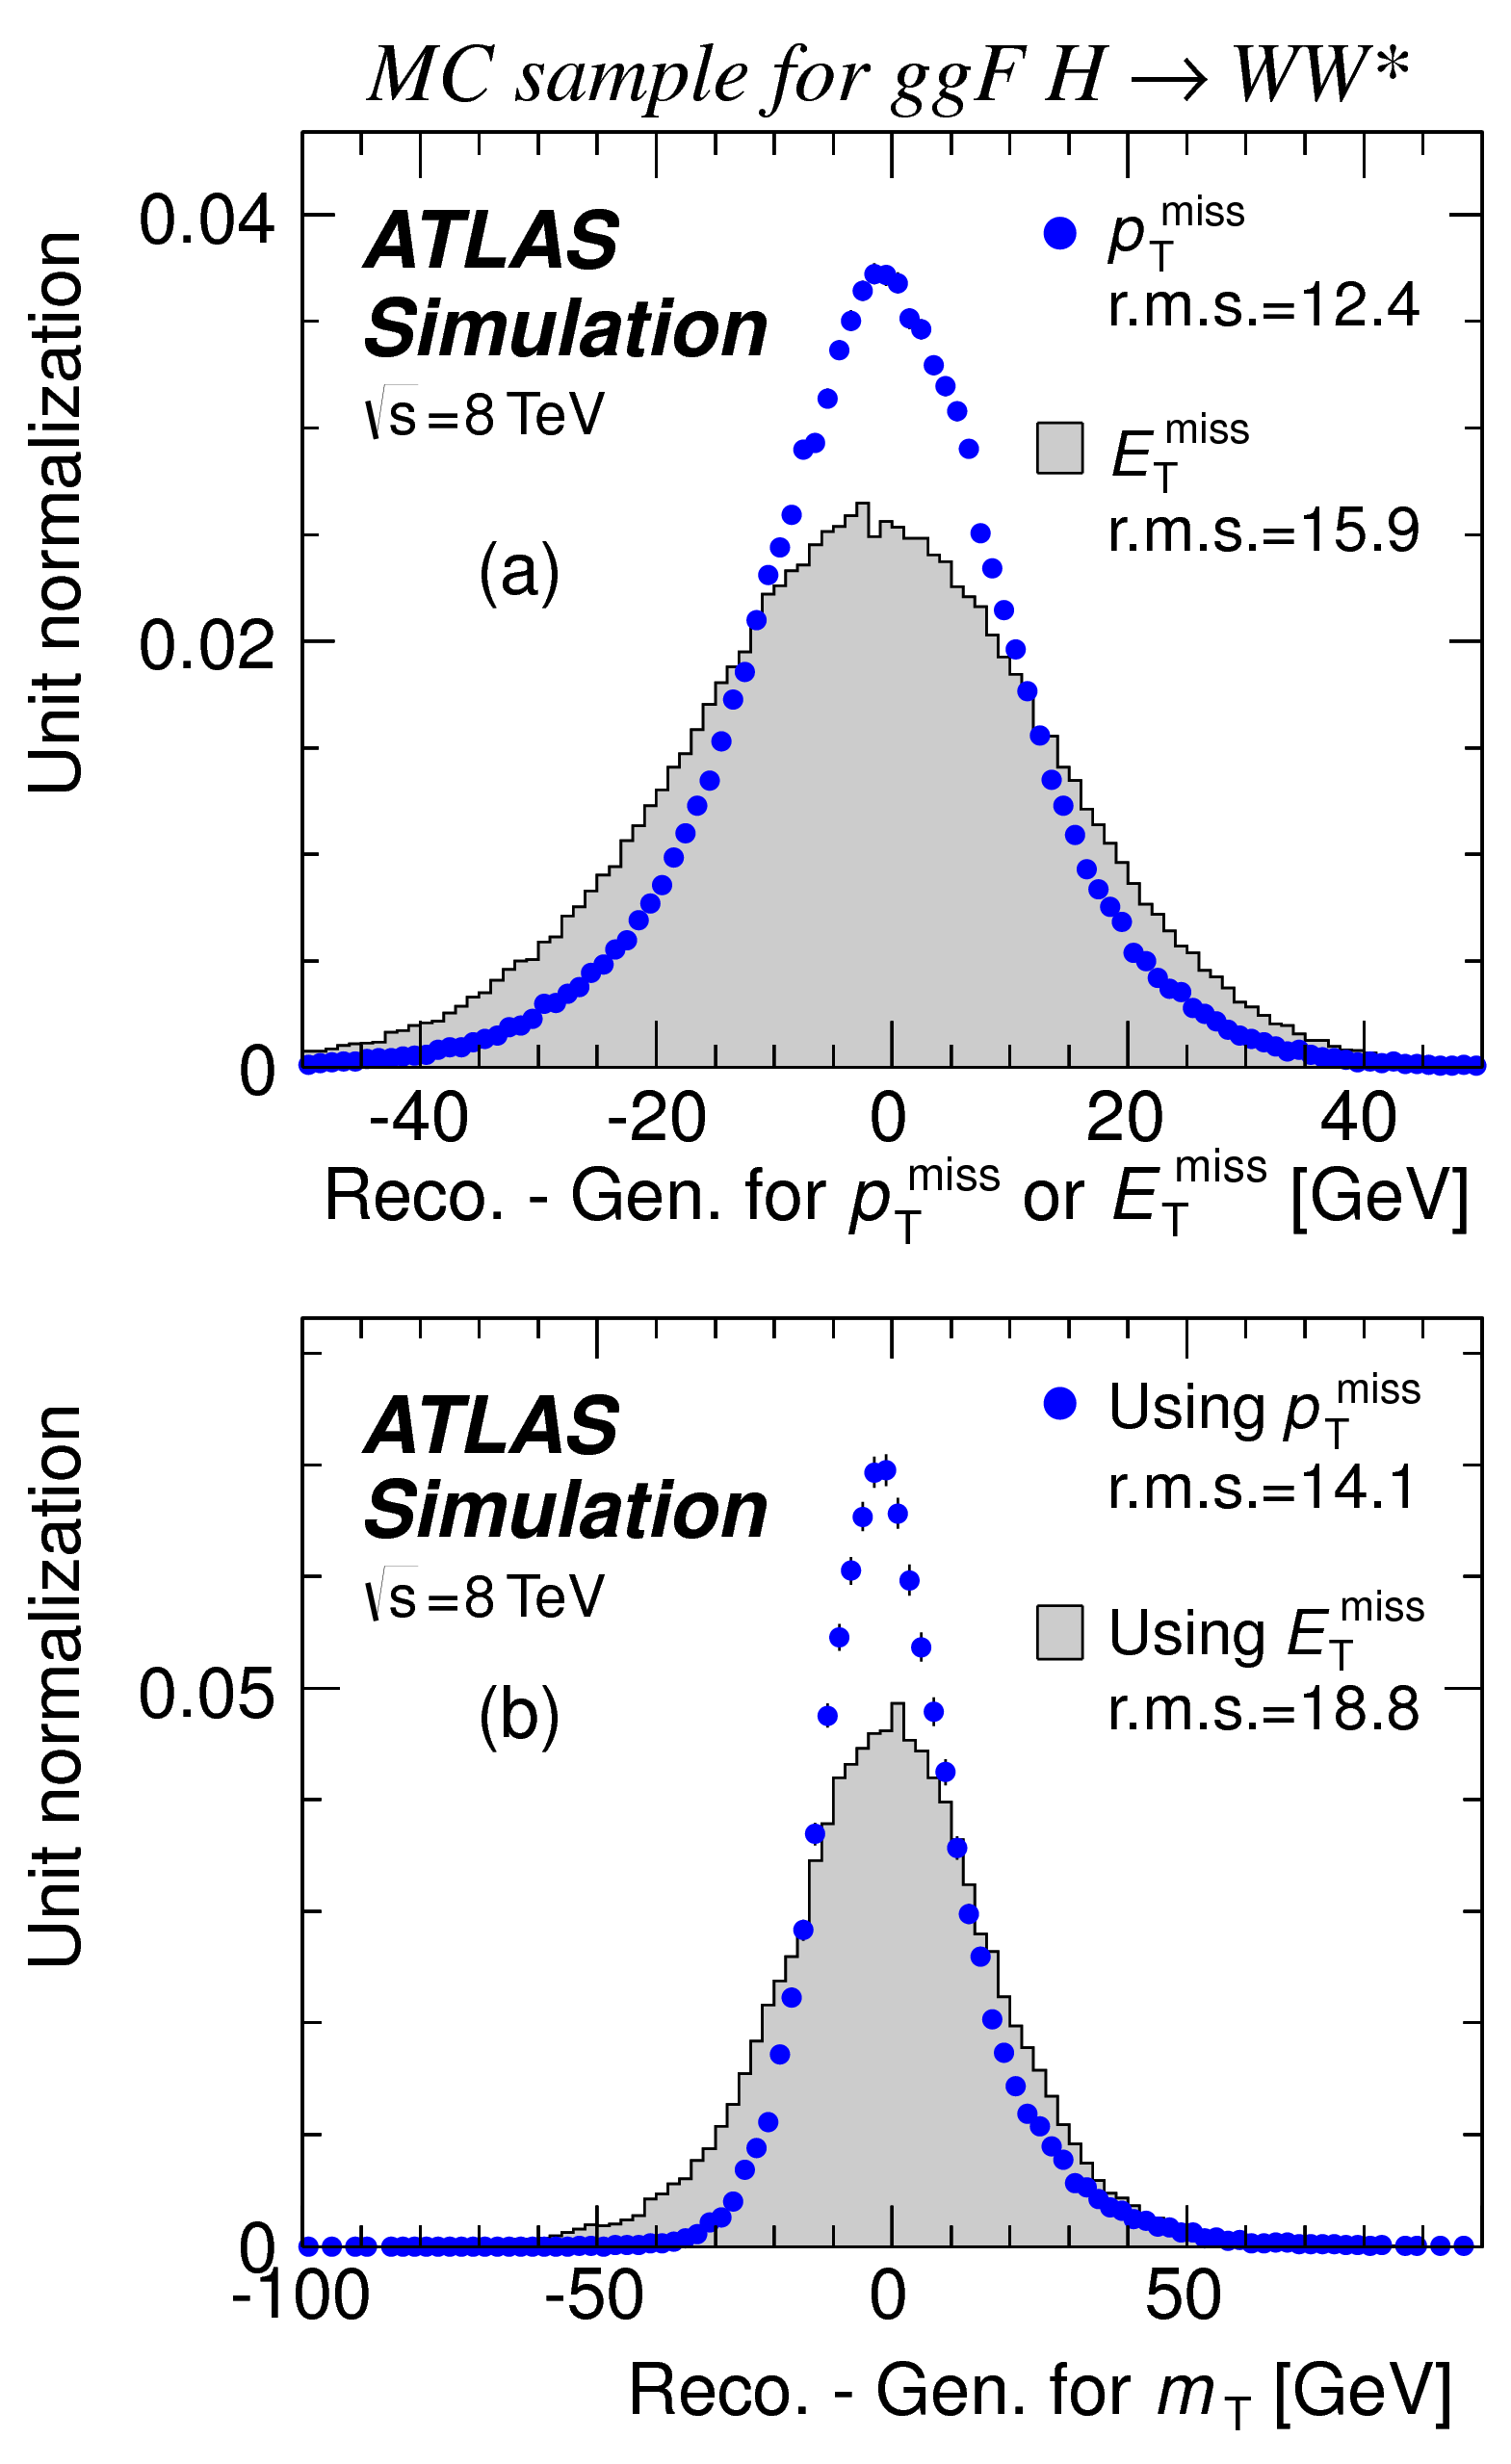
\includegraphics[width=0.6\textwidth]{figures/METResolution2}
  \caption{The difference between the true and reconstructed values of the \met (a) and $\mT$ (b) in a gluon fusion signal sample}
  \label{fig:METResolution2}
\end{figure}

Figure~\ref{fig:METResolution2}a shows the difference between the true and reconstructed values of \met using both the track-based $\MPTj$ and calorimeter based $\MET$. The RMS of the distribution improves by 3.5 \GeV when using $\MPTj$.

\subsection{Distinguishing $\ZDY$ +jets and $\HWW$ topologies}

The track-based definitions of \met were constructed to mitigate degrading performance as a function of pileup. However, an additional variable can be constructed to exploit kinematic and topological differences between the $\ZDY$ background and $\HWW$ signal. Because there are no real neutrinos in the final state (in the case of $Z/\gamma^{*} \TO ee,\mu\mu$ decays), the dilepton system of a $\ZDY$ will be balanced with the jets produced in the hard scatter. A new variable, $\frecoil$, is constructed to estimate the balance between the dilepton system and the jets in the quadrant opposite the dilepton vector in the transverse plane. It is defined in equation~\ref{eqn:frecoil}. The numerator of $\frecoil$ is the magnitude of the vectorial sum of the $\pt$ of jets in the quadrant opposite the dilepton system, weighted by each jet's Jet Vertex Fraction (JVF, described in chapter 2). The denominator is the magnitude of the dilepton $\pt$. 

\begin{equation}
\frecoil = \raisebox{-3pt}{\bigg|} \sum_{{\rm jets\,}j{\rm\,in\,}\wedge}
           \no\jvf_{\,j}\cdot\vpTjet
           ~\raisebox{-3pt}{\bigg|}
           ~\raisebox{-3pt}{\bigg/} \pTll.
\label{eqn:frecoil}
\end{equation}

Figure~\ref{fig:frecoil} shows a shape comparison of the distribution of $\frecoil$ in a simulated $\ZDY$ + jets sample, a $\HWW$ signal sample, and other backgrounds that contain real neutrinos. The $\ZDY$ + jets events tend to be more balanced between the dilepton system and recoiling jets, while the processes containing real neutrinos are less balanced in the transverse plane. Thus, a cut on $\frecoil$ will also reduce the $\ZDY$ + jets background while maintaining a good signal efficiency. 

\begin{figure}[h!]
  %\vspace{20pt}
  \centering
  \captionsetup{justification=centering}

  %\hspace*{-32pt}
  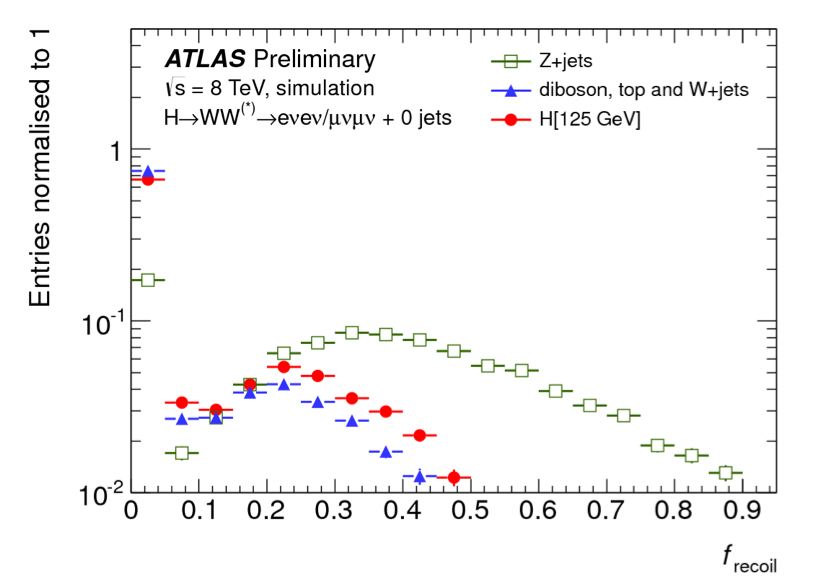
\includegraphics[width=0.6\textwidth]{figures/frecoil}
  \caption{Comparison of $\frecoil$ distributions for $\ZDY$+jets, $\HWW$, and other backgrounds with real neutrinos.}
  \label{fig:frecoil}
\end{figure}

\subsection{Optimizing background reduction cuts}

The cuts on $\MPT$ and $\frecoil$ used to reduce the Z+jets background must be optimized to maximize their efficacy. Figure~\ref{fig:optimization} shows an early attempt to optimize the combination of the two cuts in the gluon fusion zero jet bin. Each bin shows the expected signal significance if the $\MPTrel$ is required to be greater than the left edge of the bin and the $\frecoil$ is required to be less than the top edge of the bin. The figure shows that the best signal significance comes from requiring low values of $\frecoil$ ($< 0.05$) and $\MPTrel$  values greater than 45 GeV. 

\begin{figure}[h!]
  %\vspace{20pt}
  \centering
  \captionsetup{justification=centering}

  %\hspace*{-32pt}
  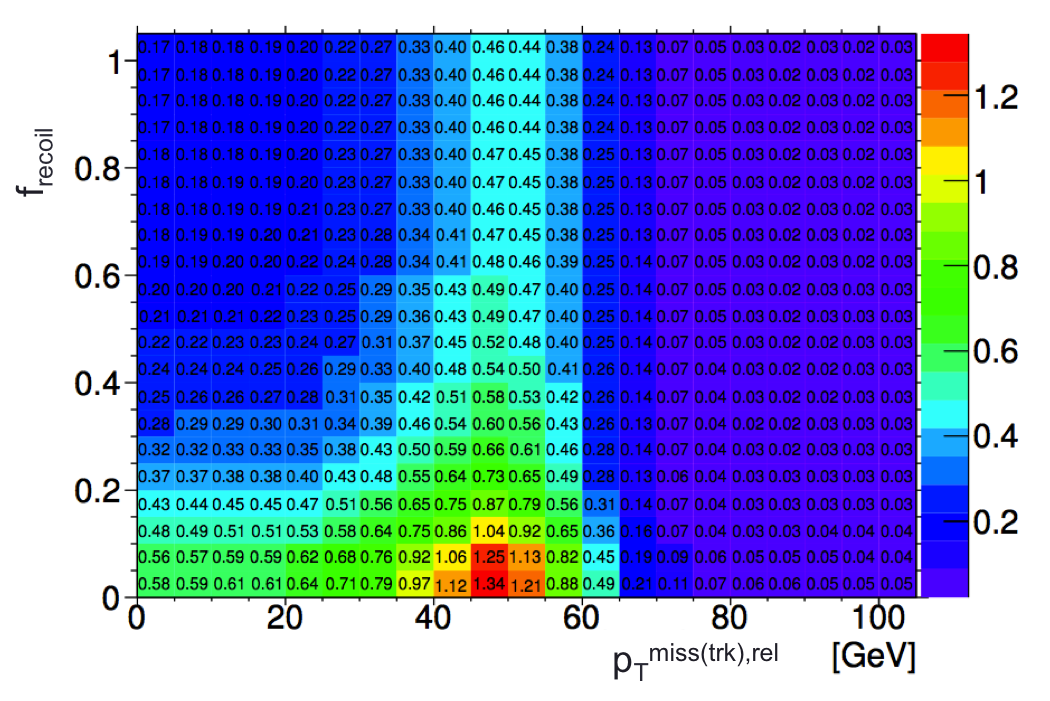
\includegraphics[width=0.8\textwidth]{figures/SFoptimization}
  \caption{Signal significance as a function of cut value in the ggF $\HWW$ with $\Njet = 0$}
  \label{fig:optimization}
\end{figure}


\section{Parameters of interest and statistical treatment}
 
As with any search or measurement, there are particular parameters of the Higgs that the $\HWW$ analysis is interested in measuring. In this case, the parameters of interest are the mass of the Higgs boson and its production cross section. Because the \HWWfull process does not have a closed final state, it is not possible to measure the full invariant mass of the particle that may have produced the final state. However, a proxy for the invariant mass using transverse plane information can be defined. This is described in more detail in section~\ref{sec:mt}. The second parameter of interest is the ratio of the measured cross section to that expected from the Standard Model Higgs, which is denoted a $\mu$. This is defined in equation~\ref{eqn:mu}.

\begin{equation}
\mu = \frac{\sigma}{\sigma_{\rm SM}}
\label{eqn:mu}
\end{equation}

All of the likelihoods used in the statistical analysis of the final signal region events are paramaterized as a function of $\mu$. $\mu$ is a natural variable for hypothesis testing, as $\mu = 0$ corresponds to a background only hypothesis and $\mu = 1$ corresponds exactly to a Standard Model Higgs. 

\subsection{Transverse mass}
\label{sec:mt}
Because the longitudinal information about the neutrinos is not attainable, the \HWWfull analysis uses a mass variable, the transverse mass, that exploits information in the transverse plane as a proxy for the full invariant mass. The transverse mass is defined in equation~\ref{eqn:mt}.

\begin{equation}
  \mTH = \sqrt{\left(\eTll + \MPTj\right)^2 - \left|\,\vpTll + \vMPTj\,\right|^2},
\label{eqn:mt}
\end{equation}

Here the $\eTll$ and $\pTll$ are the transverse energy and momentum of the dilepton system, while $\MPTj$ is a proxy for the transverse momentum of the di-neutrino system. The track-based $\MPTj$ is used in the $\mTH$ rather than the calorimeter based $\MET$ because it has a better resolution on the true transverse mass. Figure~\ref{fig:METResolution2}b shows the improvement in the RMS of the difference between the true and reconstructed transverse mass in a ggF signal sample. The RMS improves by 4.7 \GeV using $\MPTj$ in the $\mTH$ calculation.

\subsection[title]{Statistical treatment\footnote{Many thanks to Aaron Armbruster, whose thesis\cite{ArmbrusterThesis} inspired parts of this section.}} 

\subsubsection{Likelihood function}

The statistical analysis of final event candidates is framed as a hypothesis test, where the null hypothesis is background-only (no Standard Model Higgs). The first step in the analysis is to form a likelihood function for the data. In its simplest form, this likelihood is the probability of observing the number of events seen in the final signal region given knowledge of the signal strength. Because observation of events is fundamentally a Poisson counting experiment, this simple likelihood can be expressed as a Poisson probability of observing $N$ events given a total number of predicted signal and background events. This basic likelihood is shown in equation~\ref{eqn:simplepoisson}.

\begin{equation}
\likelihood(\mu) = P\left(N | \mu S + B\right)
\label{eqn:simplepoisson}
\end{equation}

Here, $P$ is the Poisson probability density function, $N$ is the total number of observed events, $\mu$ is the signal strength, $S$ is the predicted number of signal events, and $B$ is the predicted number of background events. 

In particle physics, certain background estimates are commonly normalized in so-called ``control" regions and those predictions are scaled by the same normalization factor in the signal region. This leads to a slightly more complicated likelihood, which is a function of both the signal strength and the background normalization. This is shown in equation~\ref{eqn:mediumpoisson}.

\begin{equation}
\likelihood(\mu, \theta) = P\left(N | \mu S + \theta B\right)P\left(N_{\rm CR} | \theta B_{\rm CR}\right)
\label{eqn:mediumpoisson}
\end{equation}

Here, $\theta$ is a so-called ``nuisance parameter", a parameter that is not a primary parameter of interest but still enters the likelihood. The second Poisson term adds an extra term to the likelihood, enforcing the fact that the background normalization must be consistent with the number of observed events in data in the control region, $N_{\rm CR}$.

So far, these two formulations of likelihoods have assumed a single signal region and do not take into account any shape information of potential discriminating variables. The $\HWW$ analysis is divided into many different categories, and we can perform the same counting experiment described above in each individual category. As mentioned in section~\ref{sec:mt}, the transverse mass is used as the primary discriminating variable in many of the $\HWW$ sub-analyses, so additionally we can perform the same counting experiment in each bin of the $\mTH$ distribution to incorporate some shape information. Thus, the total likelihood becomes a product over signal regions and bins of the $\mTH$ distribution. Finally, there are usually many backgrounds that are normalized in control regions, so the new formulation of the likelihood takes this into account as well by including a product over control regions in the second Poisson term. All of these modifications are shown in equation~\ref{eqn:binnedpoisson}. 

\begin{equation}
\likelihood\left(\mu, \MBF{\theta}\right) = \prod_{\substack{\rm{SRs }\, i \\ \rm{bins }\, b}} P\left(N_{ib} \Bigg| \mu S_{ib} + \sum_{\rm{bkg }\, k}\theta_{k} B_{kib}\right)
 \prod_{\substack{\rm{CRs} \, l}} P\left(N_{l} \Bigg| \sum_{\rm{bkg }\, k}\theta_{k} B_{kl}\right)
\label{eqn:binnedpoisson}
\end{equation}

The final step to get the full likelihood used in the analysis is to add nuisance parameters for the systematic uncertainties. In cases where the uncertainty does not affect the shape of $\mTH$ bin-by-bin, each systematic uncertainty $\epsilon$ is allowed to affect the expected event yields through a linear response function of the nuisance parameter, namely $\nu(\theta) = (1 + \epsilon)^\theta$. If instead the uncertainty does affect the shape, the effect is instead parameterized by $\nu_b(\theta) = 1 + \epsilon_{b}\theta$. The value of the nuisance parameters for the systematic uncertainty are constrained with a Gaussian term that is added to the likelihood as well. This is of the form $g(\delta | \theta) = e^{-(\delta - \theta)^2/2}/\sqrt{2\pi}$, where $\delta$ is the central value and $\theta$ is a nuisance parameter. Finally, a last term is added to account for the statistical uncertainty in the Monte Carlo samples used, which adds an additional poisson term. The full likelihood used in the final statistical analysis is defined in equation~\ref{eqn:fullpoisson}.

\begin{equation}
\begin{aligned}
\likelihood\left(\mu, \MBF{\theta}\right) = & \prod_{\substack{\rm{SRs }\, i \\ \rm{bins }\, b}} P\left(N_{ib} \Bigg| \mu S_{ib} \cdot \prod_{\substack{\rm{sig.} \\ \rm{syst.} \\ r}} \nu_{br}(\theta_{r})
 + \sum_{\rm{bkg }\, k}\theta_{k} B_{kib} \cdot \prod_{\substack{\rm{bkg.} \\ \rm{syst.} \\ s}} \nu_{bs}(\theta_{s}) \right)
 \\ & \cdot \prod_{\substack{\rm{CRs} \, l}} P\left(N_{l} \Bigg| \sum_{\rm{bkg }\, k}\theta_{k} B_{kl}\right)
 \\ & \cdot \prod_{\substack{\rm syst \\ t}} g\left(\delta_{t} | \theta_{t}\right)
 \cdot \prod_{\substack{\rm bkg \, k}} P\left(\xi_k | \zeta_{k} \theta_{k}\right)
\end{aligned}
\label{eqn:fullpoisson}
\end{equation}

In the fourth term of the equation, quantifying uncertainty due to finite Monte Carlo sample size, $\xi$ represents the central value of the background prediction, $\theta$ is the associated nuisance parameter, $\zeta = (B/\delta B)^2$, where $\delta B$ is the statistical uncertainty of $B$.

The best fit value of the signal strength $\mu$ is determined by finding the values of $\mu$ and $\boldsymbol{\theta}$ that maximize the likelihood, while setting $\delta = 0$ and $\xi = \zeta$.

Once the likelihood is defined, a test statistic must be built for use in hypothesis testing.

\subsubsection{Test statistic}

To distinguish whether the data match a background only or background and signal hypothesis, a test statistic must be used. The $\HWW$ analysis used the profile likelihood technique\cite{Cowan:2010st}. The first step in formulating this test statistic is to define the profile likelihood ratio, shown in equation~\ref{eqn:proflikelihood}.

\begin{equation}
\lambda(\mu) = \frac{\likelihood\left(\mu, \hat{\theta}_\mu\right)}{\likelihood\left(\hat{\mu}, \hat{\theta}\right)}
\label{eqn:proflikelihood}
\end{equation}

Here $\hat{\theta}_\mu$ is the value of $\theta$ that maximizes the likelihood for the choice of $\mu$ being tested. Additionally, $\hat{\theta}$ and $\hat{\mu}$ represent the values of $\theta$ and $\mu$ that gives the overall maximum value of the likelihood. 

Once this is defined, a test statistic $q_\mu$ is constructed. This is shown in equation~\ref{eqn:qmu}.

\begin{equation}
q_\mu = -2 \ln \lambda(\mu)
\label{eqn:qmu}
\end{equation}

A higher value of $q_\mu$ means that the data are more incompatible with the hypothesized value of $\mu$, and $q_0$ then corresponds to the value of the test statistic for the background only hypothesis. A $p_0$ value is then defined to quantify the compatibility between the data and the null hypothesis. The $p_0$ value is the probability of obtaining a value of $q_0$ larger than the observed value, and this is shown in equation~\ref{eqn:pzero}.

\begin{equation}
p_0 = \int_{q_0^{\rm obs}}^{\infty} f(q_\mu | \mu = 0) d q_\mu
\label{eqn:pzero}
\end{equation}

Here $f(q_\mu)$ is the probability distribution function of the test statistic. Finally, the $p_0$ value can be converted into a signal significance, using the formula in equation\ref{eqn:zscore}, or the one-sided tail of the Gaussian distribution. 

\begin{equation}
Z_0 = \sqrt{2} \text{erf}^{-1} (1-2p_0)
\label{eqn:zscore}
\end{equation}

The threshold for discovery used in particle physics is $Z_0 \geq 5$, more commonly known as a value of $5\sigma$.





\chapter{The discovery of the Higgs boson and the role of the $H\rightarrow WW^{*}\rightarrow \ell\nu\ell\nu$ channel}

\chapter{Observation of Vector Boson Fusion production of $H\rightarrow WW^{*}\rightarrow \ell\nu\ell\nu$}

\chapter{Combined Run 1 $H\rightarrow WW^{*}\rightarrow \ell\nu\ell\nu$results}

\part{Search for Higgs pair production in the $HH\rightarrow
  b\bar{b}b\bar{b}$ channel in LHC Run 2 at $\sqrt{s}$ = 13 TeV}

\chapter{Search overview}

\chapter{Search for Higgs pair production in boosted final states}

\chapter{Search for Higgs pair production in resolved final states}

\chapter{Combined results with Run 2 2015 dataset}

\part{Looking ahead}
\chapter{Conclusion}
\label{conclusion}

We found the Higgs. Then measured it. Then used it to look for new physics. What a time to be alive!
%\begin{appendices}
%    \chapter{ATLAS New Small Wheel Upgrade}
\label{AppendixA}



%\end{appendices}

\setstretch{1.2}

% the back matter
\clearpage
\bibliography{references}
\addcontentsline{toc}{chapter}{References}
\bibliographystyle{apalike2}

\newpage

% If you do want an image in the colophon:
\begin{figure}
  \vspace{20pt}
  \centering
  \hspace*{-32pt}
  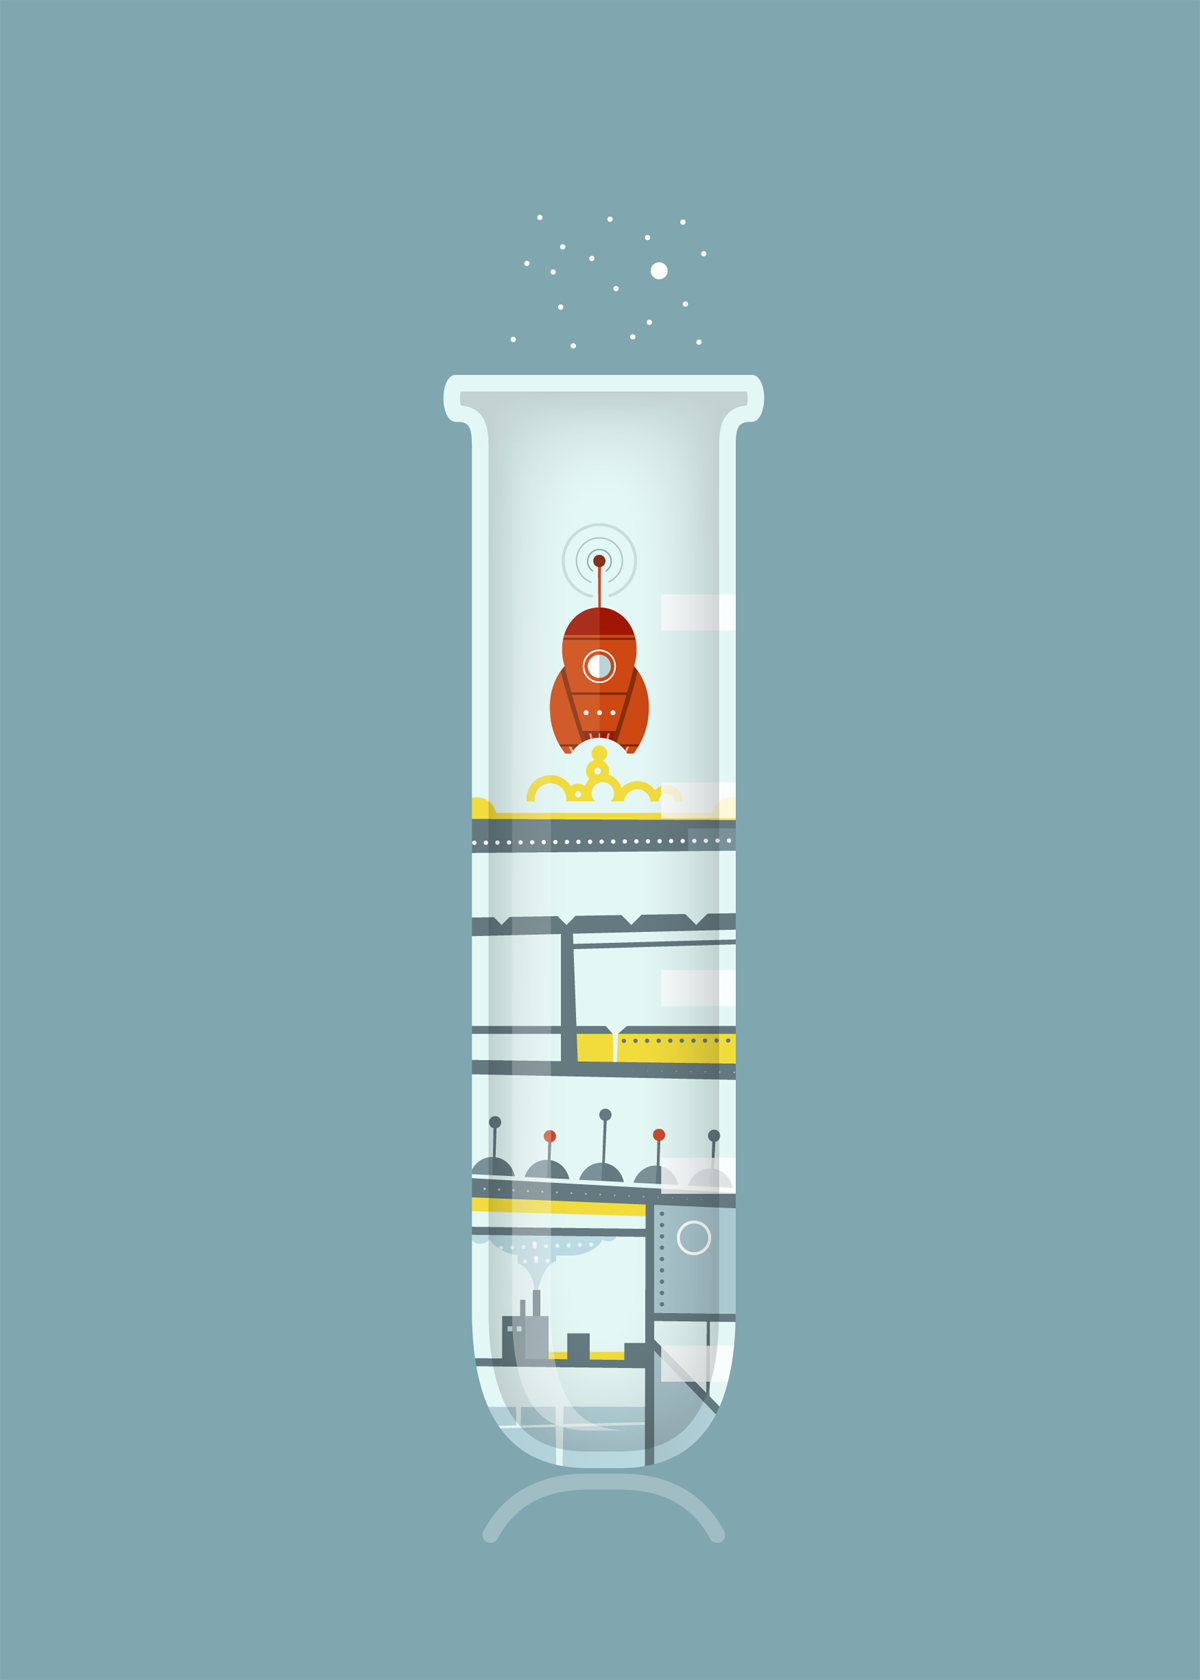
\includegraphics[width=0.42\textwidth]{endmatter/colophon.png}
\end{figure}

% If you don't want an image in the colophon:
% \vspace*{200pt}

\begin{center}
\parbox{200pt}{\lettrine[lines=3,slope=-2pt,nindent=-4pt]{\textcolor{SchoolColor}{T}}{his thesis was typeset} using \LaTeX, originally developed by Leslie Lamport and based on Donald Knuth's \TeX. The body text is set in 11 point Egenolff-Berner Garamond, a revival of Claude Garamont's humanist typeface. The above illustration, \textit{Science Experiment 02}, was created by Ben Schlitter and released under \href{http://creativecommons.org/licenses/by-nc-nd/3.0/}{\textsc{cc by-nc-nd 3.0}}. A template that can be used to format a PhD dissertation with this look \textit{\&} feel has been released under the permissive \textsc{agpl} license, and can be found online at \href{https://github.com/asm-products/Dissertate}{github.com/asm-products/Dissertate} or from its lead author, Jordan Suchow, at \href{mailto:suchow@post.harvard.edu}{suchow@post.harvard.edu}.}
\end{center}


\end{document}
